% Options for packages loaded elsewhere
\PassOptionsToPackage{unicode}{hyperref}
\PassOptionsToPackage{hyphens}{url}
%
\documentclass[
]{article}
\usepackage{lmodern}
\usepackage{amssymb,amsmath}
\usepackage{ifxetex,ifluatex}
\ifnum 0\ifxetex 1\fi\ifluatex 1\fi=0 % if pdftex
  \usepackage[T1]{fontenc}
  \usepackage[utf8]{inputenc}
  \usepackage{textcomp} % provide euro and other symbols
\else % if luatex or xetex
  \usepackage{unicode-math}
  \defaultfontfeatures{Scale=MatchLowercase}
  \defaultfontfeatures[\rmfamily]{Ligatures=TeX,Scale=1}
\fi
% Use upquote if available, for straight quotes in verbatim environments
\IfFileExists{upquote.sty}{\usepackage{upquote}}{}
\IfFileExists{microtype.sty}{% use microtype if available
  \usepackage[]{microtype}
  \UseMicrotypeSet[protrusion]{basicmath} % disable protrusion for tt fonts
}{}
\makeatletter
\@ifundefined{KOMAClassName}{% if non-KOMA class
  \IfFileExists{parskip.sty}{%
    \usepackage{parskip}
  }{% else
    \setlength{\parindent}{0pt}
    \setlength{\parskip}{6pt plus 2pt minus 1pt}}
}{% if KOMA class
  \KOMAoptions{parskip=half}}
\makeatother
\usepackage{xcolor}
\IfFileExists{xurl.sty}{\usepackage{xurl}}{} % add URL line breaks if available
\IfFileExists{bookmark.sty}{\usepackage{bookmark}}{\usepackage{hyperref}}
\hypersetup{
  pdftitle={RTP02 Exercises},
  pdfauthor={Silvia Geiser},
  hidelinks,
  pdfcreator={LaTeX via pandoc}}
\urlstyle{same} % disable monospaced font for URLs
\usepackage[margin=1in]{geometry}
\usepackage{color}
\usepackage{fancyvrb}
\newcommand{\VerbBar}{|}
\newcommand{\VERB}{\Verb[commandchars=\\\{\}]}
\DefineVerbatimEnvironment{Highlighting}{Verbatim}{commandchars=\\\{\}}
% Add ',fontsize=\small' for more characters per line
\usepackage{framed}
\definecolor{shadecolor}{RGB}{248,248,248}
\newenvironment{Shaded}{\begin{snugshade}}{\end{snugshade}}
\newcommand{\AlertTok}[1]{\textcolor[rgb]{0.94,0.16,0.16}{#1}}
\newcommand{\AnnotationTok}[1]{\textcolor[rgb]{0.56,0.35,0.01}{\textbf{\textit{#1}}}}
\newcommand{\AttributeTok}[1]{\textcolor[rgb]{0.77,0.63,0.00}{#1}}
\newcommand{\BaseNTok}[1]{\textcolor[rgb]{0.00,0.00,0.81}{#1}}
\newcommand{\BuiltInTok}[1]{#1}
\newcommand{\CharTok}[1]{\textcolor[rgb]{0.31,0.60,0.02}{#1}}
\newcommand{\CommentTok}[1]{\textcolor[rgb]{0.56,0.35,0.01}{\textit{#1}}}
\newcommand{\CommentVarTok}[1]{\textcolor[rgb]{0.56,0.35,0.01}{\textbf{\textit{#1}}}}
\newcommand{\ConstantTok}[1]{\textcolor[rgb]{0.00,0.00,0.00}{#1}}
\newcommand{\ControlFlowTok}[1]{\textcolor[rgb]{0.13,0.29,0.53}{\textbf{#1}}}
\newcommand{\DataTypeTok}[1]{\textcolor[rgb]{0.13,0.29,0.53}{#1}}
\newcommand{\DecValTok}[1]{\textcolor[rgb]{0.00,0.00,0.81}{#1}}
\newcommand{\DocumentationTok}[1]{\textcolor[rgb]{0.56,0.35,0.01}{\textbf{\textit{#1}}}}
\newcommand{\ErrorTok}[1]{\textcolor[rgb]{0.64,0.00,0.00}{\textbf{#1}}}
\newcommand{\ExtensionTok}[1]{#1}
\newcommand{\FloatTok}[1]{\textcolor[rgb]{0.00,0.00,0.81}{#1}}
\newcommand{\FunctionTok}[1]{\textcolor[rgb]{0.00,0.00,0.00}{#1}}
\newcommand{\ImportTok}[1]{#1}
\newcommand{\InformationTok}[1]{\textcolor[rgb]{0.56,0.35,0.01}{\textbf{\textit{#1}}}}
\newcommand{\KeywordTok}[1]{\textcolor[rgb]{0.13,0.29,0.53}{\textbf{#1}}}
\newcommand{\NormalTok}[1]{#1}
\newcommand{\OperatorTok}[1]{\textcolor[rgb]{0.81,0.36,0.00}{\textbf{#1}}}
\newcommand{\OtherTok}[1]{\textcolor[rgb]{0.56,0.35,0.01}{#1}}
\newcommand{\PreprocessorTok}[1]{\textcolor[rgb]{0.56,0.35,0.01}{\textit{#1}}}
\newcommand{\RegionMarkerTok}[1]{#1}
\newcommand{\SpecialCharTok}[1]{\textcolor[rgb]{0.00,0.00,0.00}{#1}}
\newcommand{\SpecialStringTok}[1]{\textcolor[rgb]{0.31,0.60,0.02}{#1}}
\newcommand{\StringTok}[1]{\textcolor[rgb]{0.31,0.60,0.02}{#1}}
\newcommand{\VariableTok}[1]{\textcolor[rgb]{0.00,0.00,0.00}{#1}}
\newcommand{\VerbatimStringTok}[1]{\textcolor[rgb]{0.31,0.60,0.02}{#1}}
\newcommand{\WarningTok}[1]{\textcolor[rgb]{0.56,0.35,0.01}{\textbf{\textit{#1}}}}
\usepackage{graphicx,grffile}
\makeatletter
\def\maxwidth{\ifdim\Gin@nat@width>\linewidth\linewidth\else\Gin@nat@width\fi}
\def\maxheight{\ifdim\Gin@nat@height>\textheight\textheight\else\Gin@nat@height\fi}
\makeatother
% Scale images if necessary, so that they will not overflow the page
% margins by default, and it is still possible to overwrite the defaults
% using explicit options in \includegraphics[width, height, ...]{}
\setkeys{Gin}{width=\maxwidth,height=\maxheight,keepaspectratio}
% Set default figure placement to htbp
\makeatletter
\def\fps@figure{htbp}
\makeatother
\setlength{\emergencystretch}{3em} % prevent overfull lines
\providecommand{\tightlist}{%
  \setlength{\itemsep}{0pt}\setlength{\parskip}{0pt}}
\setcounter{secnumdepth}{-\maxdimen} % remove section numbering

\title{RTP02 Exercises}
\author{Silvia Geiser}
\date{01/2021}

\begin{document}
\maketitle

{
\setcounter{tocdepth}{2}
\tableofcontents
}
\hypertarget{introduction}{%
\section{Introduction}\label{introduction}}

\hypertarget{create-time-series}{%
\subsection{Create Time Series}\label{create-time-series}}

What is the expected period (time period of repetition) and the time
step for the following timeseries:

\begin{Shaded}
\begin{Highlighting}[]
\NormalTok{dat =}\StringTok{ }\KeywordTok{floor}\NormalTok{(}\KeywordTok{runif}\NormalTok{(}\DataTypeTok{n=} \DecValTok{1000}\NormalTok{, }\DataTypeTok{min =} \DecValTok{1}\NormalTok{, }\DataTypeTok{max=} \DecValTok{2000}\NormalTok{))}
\end{Highlighting}
\end{Shaded}

\begin{enumerate}
\def\labelenumi{\alph{enumi})}
\tightlist
\item
  Sunshine duration per month in Basel from 1990 to 2000
\end{enumerate}

\begin{Shaded}
\begin{Highlighting}[]
\KeywordTok{ts}\NormalTok{(}\DataTypeTok{data =}\NormalTok{ dat, }\DataTypeTok{start=}\KeywordTok{c}\NormalTok{(}\DecValTok{1990}\NormalTok{,}\DecValTok{1}\NormalTok{),}\DataTypeTok{end=}\KeywordTok{c}\NormalTok{(}\DecValTok{2000}\NormalTok{,}\DecValTok{12}\NormalTok{), }\DataTypeTok{frequency =} \DecValTok{12}\NormalTok{)}
\end{Highlighting}
\end{Shaded}

\begin{enumerate}
\def\labelenumi{\alph{enumi})}
\setcounter{enumi}{1}
\tightlist
\item
  Number of newborn babies in the city of Zurich per year from 2000 to
  2011
\end{enumerate}

\begin{Shaded}
\begin{Highlighting}[]
\KeywordTok{ts}\NormalTok{(}\DataTypeTok{data=}\NormalTok{dat, }\DataTypeTok{start=}\DecValTok{2000}\NormalTok{,}\DataTypeTok{end=}\DecValTok{2011}\NormalTok{,}\DataTypeTok{frequency =} \DecValTok{1}\NormalTok{)}
\end{Highlighting}
\end{Shaded}

c)Number of reservations in a restaurant for every night during 4 weeks

\begin{Shaded}
\begin{Highlighting}[]
\KeywordTok{ts}\NormalTok{(}\DataTypeTok{data=}\NormalTok{dat, }\DataTypeTok{start=}\DecValTok{1}\NormalTok{,}\DataTypeTok{end=}\DecValTok{4}\NormalTok{,}\DataTypeTok{frequency =} \DecValTok{7}\NormalTok{)}
\end{Highlighting}
\end{Shaded}

\begin{enumerate}
\def\labelenumi{\alph{enumi})}
\setcounter{enumi}{3}
\tightlist
\item
  Water runoff of a river. The data has been collected every day for 4
  years
\end{enumerate}

\begin{Shaded}
\begin{Highlighting}[]
\KeywordTok{ts}\NormalTok{(}\DataTypeTok{data=}\NormalTok{dat, }\DataTypeTok{start=}\DecValTok{1}\NormalTok{,}\DataTypeTok{end=}\DecValTok{4}\NormalTok{,}\DataTypeTok{frequency =} \DecValTok{365}\NormalTok{)}
\end{Highlighting}
\end{Shaded}

\hypertarget{simulate-time-series}{%
\subsection{Simulate Time Series}\label{simulate-time-series}}

\begin{Shaded}
\begin{Highlighting}[]
\NormalTok{zeitsim <-}\StringTok{ }\KeywordTok{read.table}\NormalTok{(}\StringTok{'https://stat.ethz.ch/Teaching/Datasets/WBL/zeitsim.dat'}\NormalTok{)}
\NormalTok{zeitsim.ts <-}\StringTok{ }\KeywordTok{ts}\NormalTok{(zeitsim[,}\DecValTok{1}\OperatorTok{:}\DecValTok{4}\NormalTok{], }\DataTypeTok{start =} \DecValTok{1}\NormalTok{, }\DataTypeTok{frequency =} \DecValTok{1}\NormalTok{)}
\end{Highlighting}
\end{Shaded}

Simulate timeseries according to the following models:

\begin{Shaded}
\begin{Highlighting}[]
\KeywordTok{set.seed}\NormalTok{(}\DecValTok{100}\NormalTok{)}
\NormalTok{Et <-}\StringTok{ }\KeywordTok{ts}\NormalTok{(}\KeywordTok{rnorm}\NormalTok{(}\DecValTok{101}\NormalTok{, }\DecValTok{0}\NormalTok{, }\DecValTok{1}\NormalTok{))}
\NormalTok{Et [}\DecValTok{1}\NormalTok{] <-}\StringTok{ }\DecValTok{0}
\NormalTok{y1 <-}\StringTok{ }\DecValTok{0}

\ControlFlowTok{for}\NormalTok{ (i }\ControlFlowTok{in} \DecValTok{2}\OperatorTok{:}\KeywordTok{length}\NormalTok{(Et)) \{}
\NormalTok{  y1[i] <-}\StringTok{ }\NormalTok{Et[i]}
\NormalTok{  \}}

\NormalTok{y1 <-}\StringTok{ }\NormalTok{y1[}\DecValTok{2}\OperatorTok{:}\KeywordTok{length}\NormalTok{(y1)]}
\NormalTok{ts.y1 <-}\StringTok{ }\KeywordTok{ts}\NormalTok{(y1)}
\end{Highlighting}
\end{Shaded}

\textbf{a) Y1: Yt = Et − 0.5 · Et−1 , where Et ∼ N(0, 1) i.i.d. E0 = 0}

\begin{Shaded}
\begin{Highlighting}[]
\KeywordTok{set.seed}\NormalTok{(}\DecValTok{100}\NormalTok{)}
\NormalTok{Et <-}\StringTok{ }\KeywordTok{ts}\NormalTok{(}\KeywordTok{rnorm}\NormalTok{(}\DecValTok{101}\NormalTok{,}\DecValTok{0}\NormalTok{,}\DecValTok{1}\NormalTok{))}
\NormalTok{Et [}\DecValTok{1}\NormalTok{] <-}\StringTok{ }\DecValTok{0}
\NormalTok{y1 <-}\StringTok{ }\DecValTok{0}
\ControlFlowTok{for}\NormalTok{ (i }\ControlFlowTok{in} \DecValTok{2}\OperatorTok{:}\KeywordTok{length}\NormalTok{(Et)) \{}
\NormalTok{  y1 [i] <-}\StringTok{ }\NormalTok{Et[i] }\OperatorTok{-}\StringTok{ }\FloatTok{0.5} \OperatorTok{*}\StringTok{ }\NormalTok{Et[i}\DecValTok{-1}\NormalTok{]}
\NormalTok{\}}

\NormalTok{y1 <-}\StringTok{ }\NormalTok{y1[}\DecValTok{2}\OperatorTok{:}\KeywordTok{length}\NormalTok{(y1)]}
\NormalTok{ts.y1 <-}\StringTok{ }\KeywordTok{ts}\NormalTok{(y1)}

\KeywordTok{par}\NormalTok{(}\DataTypeTok{mfrow=} \KeywordTok{c}\NormalTok{(}\DecValTok{1}\NormalTok{,}\DecValTok{2}\NormalTok{))}
\KeywordTok{plot}\NormalTok{(ts.y1, }\DataTypeTok{lwd =} \FloatTok{1.5}\NormalTok{, }\DataTypeTok{main =} \StringTok{'Y1: Yt = Et − 0.5 · Et−1 , where Et ∼ N(0, 1) i.i.d. E0 = 0'}\NormalTok{)}
\KeywordTok{plot}\NormalTok{(zeitsim.ts[,}\DecValTok{1}\NormalTok{], }\DataTypeTok{main =} \StringTok{'Zeitsim Y1'}\NormalTok{, }\DataTypeTok{lwd =} \FloatTok{1.5}\NormalTok{)}
\end{Highlighting}
\end{Shaded}

\includegraphics{RTP02_Exercises_files/figure-latex/unnamed-chunk-8-1.pdf}

Answer:

\begin{itemize}
\item
  stationary time series
\item
  MA(1) process
\end{itemize}

\textbf{b)Y2: Yt = Yt−1 + Et, where Et ∼ N(0, 1) i.i.d. Y0 = 0}

\begin{Shaded}
\begin{Highlighting}[]
\KeywordTok{set.seed}\NormalTok{(}\DecValTok{100}\NormalTok{)}
\NormalTok{Et <-}\StringTok{ }\KeywordTok{ts}\NormalTok{(}\KeywordTok{rnorm}\NormalTok{(}\DecValTok{100}\NormalTok{,}\DecValTok{0}\NormalTok{,}\DecValTok{1}\NormalTok{))}
\NormalTok{y2 <-}\StringTok{ }\DecValTok{0}
\ControlFlowTok{for}\NormalTok{ (i }\ControlFlowTok{in} \DecValTok{2}\OperatorTok{:}\KeywordTok{length}\NormalTok{(Et)) \{}
\NormalTok{  y2[i] <-}\StringTok{ }\NormalTok{y2[i}\DecValTok{-1}\NormalTok{] }\OperatorTok{+}\StringTok{ }\NormalTok{Et[i]}
\NormalTok{\}}

\NormalTok{ts.y2 <-}\StringTok{ }\KeywordTok{ts}\NormalTok{(y2)}

\KeywordTok{par}\NormalTok{(}\DataTypeTok{mfrow =} \KeywordTok{c}\NormalTok{(}\DecValTok{1}\NormalTok{,}\DecValTok{2}\NormalTok{))}
\KeywordTok{plot}\NormalTok{(ts.y2, }\DataTypeTok{main =} \StringTok{'Y2: Yt = Yt−1 + Et, where Et ∼ N(0, 1) i.i.d. Y0 = 0'}\NormalTok{, }\DataTypeTok{lwd =} \FloatTok{1.5}\NormalTok{)}
\KeywordTok{plot}\NormalTok{(zeitsim.ts[,}\DecValTok{2}\NormalTok{], }\DataTypeTok{main =} \StringTok{'Zeitsim Y2'}\NormalTok{, }\DataTypeTok{lwd =} \FloatTok{1.5}\NormalTok{)}
\end{Highlighting}
\end{Shaded}

\includegraphics{RTP02_Exercises_files/figure-latex/unnamed-chunk-9-1.pdf}

Answer:

\begin{itemize}
\item
  non stationary time series
\item
  Yt-1 and Et are uncorrelated random variables
\end{itemize}

\textbf{c) Y3: Yt = 0.5 · Yt−1 + Et, where Et ∼ N(0, 1) i.i.d. Y0 = 0}

\begin{Shaded}
\begin{Highlighting}[]
\KeywordTok{set.seed}\NormalTok{(}\DecValTok{100}\NormalTok{)}
\NormalTok{Et <-}\StringTok{ }\KeywordTok{ts}\NormalTok{(}\KeywordTok{rnorm}\NormalTok{(}\DecValTok{100}\NormalTok{,}\DecValTok{0}\NormalTok{,}\DecValTok{1}\NormalTok{))}
\NormalTok{y3 <-}\StringTok{ }\DecValTok{0}
\ControlFlowTok{for}\NormalTok{ (i }\ControlFlowTok{in} \DecValTok{2}\OperatorTok{:}\KeywordTok{length}\NormalTok{(Et)) \{}
\NormalTok{  y3[i] <-}\StringTok{ }\FloatTok{0.5} \OperatorTok{*}\StringTok{ }\NormalTok{y3[i }\OperatorTok{-}\StringTok{ }\DecValTok{1}\NormalTok{] }\OperatorTok{+}\StringTok{ }\NormalTok{Et[i]}
\NormalTok{\}}

\NormalTok{ts.y3 <-}\StringTok{ }\KeywordTok{ts}\NormalTok{(y3)}

\KeywordTok{par}\NormalTok{(}\DataTypeTok{mfrow =} \KeywordTok{c}\NormalTok{(}\DecValTok{1}\NormalTok{,}\DecValTok{2}\NormalTok{))}
\KeywordTok{plot}\NormalTok{(ts.y3, }\DataTypeTok{lwd =} \FloatTok{1.5}\NormalTok{, }\DataTypeTok{main=} \StringTok{'Y3: Yt = 0.5 · Yt−1 + Et, where Et ∼ N(0, 1) i.i.d. Y0 = 0'}\NormalTok{)}
\KeywordTok{plot}\NormalTok{(zeitsim.ts[,}\DecValTok{3}\NormalTok{], }\DataTypeTok{main =} \StringTok{'Zeitsim Y3'}\NormalTok{, }\DataTypeTok{lwd =} \FloatTok{1.5}\NormalTok{)}
\end{Highlighting}
\end{Shaded}

\includegraphics{RTP02_Exercises_files/figure-latex/unnamed-chunk-10-1.pdf}

Answer:

\begin{itemize}
\item
  stationary time series
\item
  AR(1) process
\end{itemize}

\textbf{d) Y4: Yt = Yt−1 · Et, where Et ∼ U(0.95, 1.05) i.i.d. Y0 = 1}

\begin{Shaded}
\begin{Highlighting}[]
\KeywordTok{set.seed}\NormalTok{(}\DecValTok{100}\NormalTok{)}
\NormalTok{Et <-}\StringTok{ }\KeywordTok{ts}\NormalTok{(}\KeywordTok{runif}\NormalTok{(}\DecValTok{100}\NormalTok{,}\FloatTok{0.95}\NormalTok{, }\FloatTok{1.05}\NormalTok{))}
\NormalTok{y4 <-}\StringTok{ }\DecValTok{1}
\ControlFlowTok{for}\NormalTok{ (i }\ControlFlowTok{in} \DecValTok{2}\OperatorTok{:}\KeywordTok{length}\NormalTok{(Et)) \{}
\NormalTok{  y4[i] <-}\StringTok{ }\NormalTok{y4[i}\DecValTok{-1}\NormalTok{] }\OperatorTok{*}\StringTok{ }\NormalTok{Et[i]}
\NormalTok{\}}

\NormalTok{ts.y4 <-}\StringTok{ }\KeywordTok{ts}\NormalTok{(y4)}

\KeywordTok{par}\NormalTok{(}\DataTypeTok{mfrow=} \KeywordTok{c}\NormalTok{(}\DecValTok{1}\NormalTok{,}\DecValTok{2}\NormalTok{))}
\KeywordTok{ts.plot}\NormalTok{(ts.y4, }\DataTypeTok{main =}\StringTok{'Y4: Yt = Yt−1 · Et, where Et ∼ U(0.95, 1.05) i.i.d. Y0 = 1'}\NormalTok{, }\DataTypeTok{lwd =} \FloatTok{1.5}\NormalTok{)}
\KeywordTok{plot}\NormalTok{(zeitsim.ts[,}\DecValTok{4}\NormalTok{], }\DataTypeTok{main =} \StringTok{'Zeitsim Y4'}\NormalTok{, }\DataTypeTok{lwd =} \FloatTok{1.5}\NormalTok{)}
\end{Highlighting}
\end{Shaded}

\includegraphics{RTP02_Exercises_files/figure-latex/unnamed-chunk-11-1.pdf}

Answer:

\begin{itemize}
\tightlist
\item
  non stationary time series, as Var(Yt) is NOT constant
\end{itemize}

\hypertarget{transformation}{%
\section{Transformation}\label{transformation}}

\begin{itemize}
\item
  Linear transformation (mostly for unit/range conversion)
\item
  Log transformation (to reduce right-skewedness in data distribution)
\end{itemize}

\hypertarget{stationarity}{%
\subsection{Stationarity}\label{stationarity}}

A stationary time series is one whose properties do not depend on the
time at which the series is observed. Thus, time series with trends, or
with seasonality, are not stationary --- the trend and seasonality will
affect the value of the time series at different times. A white noise
series is stationary --- it does not matter when you observe it, it
should look much the same at any point in time.

Some cases can be confusing --- a time series with cyclic behaviour (but
with no trend or seasonality) is stationary. This is because the cycles
are not of a fixed length, so before we observe the series we cannot be
sure where the peaks and troughs of the cycles will be.

In general, a stationary time series will have no predictable patterns
in the long-term. Time plots will show the series to be roughly
horizontal (although some cyclic behaviour is possible), with constant
variance.

\hypertarget{testing-stationarity}{%
\subsubsection{Testing Stationarity}\label{testing-stationarity}}

\begin{itemize}
\item
  Only the time series process can be tested for stationarity not the
  realization
\item
  Augmented Dickey-Fuller test
\item
  Phillips-Perron Test
\item
  KPSS Test
\item
  Elliot Rothenberg-Stock
\item
  Schmidt-Phillips
\item
  Zivot-Andrews
\end{itemize}

\hypertarget{skewness}{%
\subsection{Skewness}\label{skewness}}

The direction of the skew is dependent on whether the bulk of the
material is above the mean line (negative skew) or below the mean line
(positive skew).

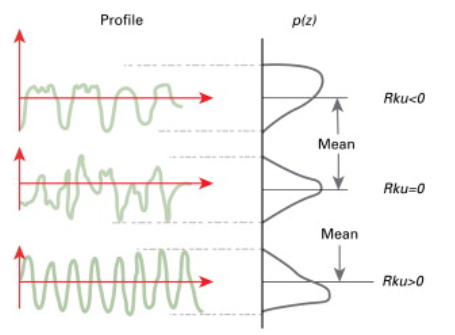
\includegraphics[width=0.5\linewidth]{skewness}

\hypertarget{linear-transformation}{%
\subsection{Linear Transformation}\label{linear-transformation}}

\textbf{Yt = mXt + b} with \textbf{m} and \textbf{b} as constants. Used
for conversion of units:

CHF to EURO Km to meters Joule to Kilowatt-hours

Linear transformations only scale key properties such as
autocorrelations, models and forecasts.

\hypertarget{log-transformation}{%
\subsection{Log Transformation}\label{log-transformation}}

\textbf{gt = log(Xt)}

Used for right-skewed time series distributation or if the data show
variation that increases or decreases with the level of the series, then
a transformation can be useful. Logarithms can help to stabilise the
variance of a time series. For example, if we denote the original
observations as y1,\ldots,yT and the transformed observations as
w1,\ldots,wT, then wt=log(yt). Logarithms are interpretable: changes in
a log value are relative (or percentage) changes on the original scale.
So if log base 10 is used, then an increase of 1 on the log scale
corresponds to a multiplication of 10 on the original scale. Another
useful feature of log transformations is that they constrain the
forecasts to stay positive on the original scale.

Example (log is the logarithm to the base 10), i.e.~ log(1) = 0 log(10)
= 1 log(100) =2 log(1000)=3 and so forth.

This means that the logarithm squezes all values between 1 and 10 to the
range between 0 and 1, all values between 10 and 100 to the range
between 1 and 2, and all values between 100 and 1000 to the range
between 2 and 3. In conclusion, the higher the values get, the more the
logarithm squeezes them together.

\hypertarget{box-cox-transformation}{%
\subsection{Box-Cox Transformation}\label{box-cox-transformation}}

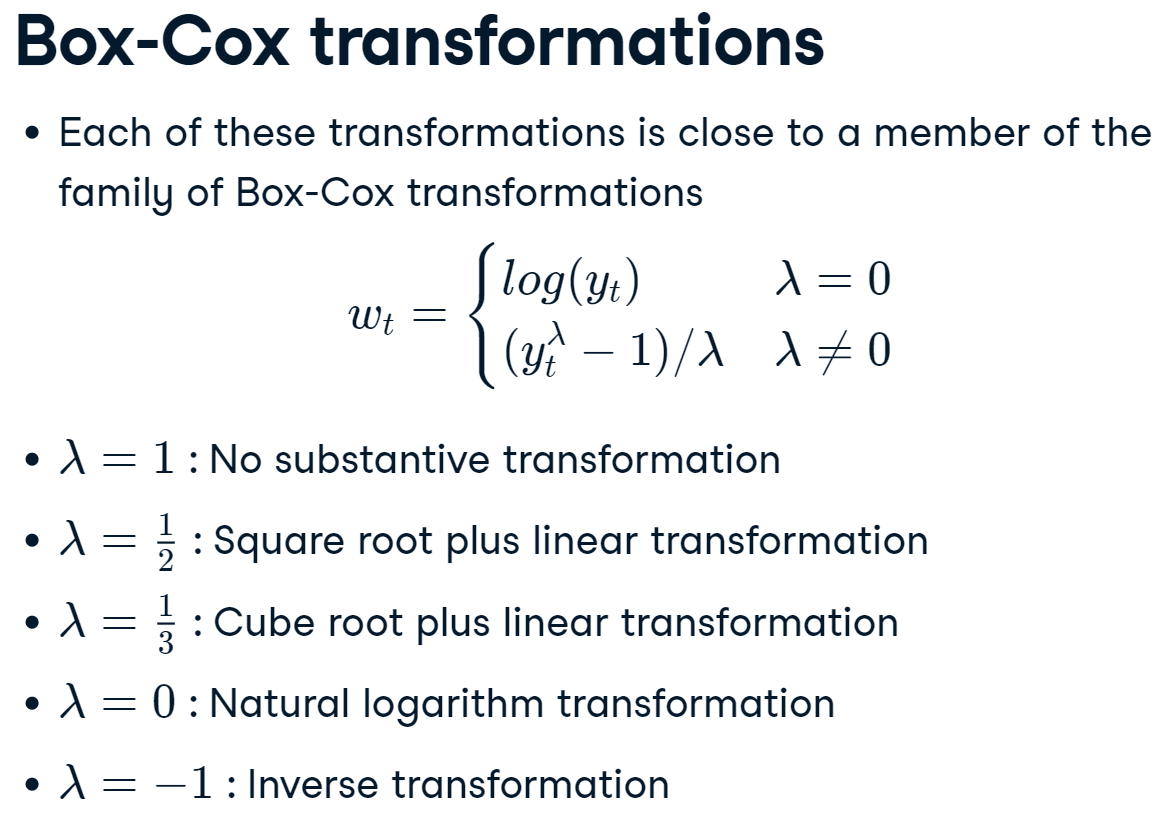
\includegraphics[width=1\linewidth]{box}

R-code: BoxCox.lambda(data)

\hypertarget{methods-for-trend-determinationelimination}{%
\section{Methods for trend
determination/elimination}\label{methods-for-trend-determinationelimination}}

\begin{itemize}
\item
  (linear) fitting, e.g.~with ordinary least square fitting
\item
  (Backwards) differencing (higher order differences eliminate higher
  order polynomial trends)
\item
  filtration
\end{itemize}

\textbf{Advantages and drawbacks of the individual procedures}

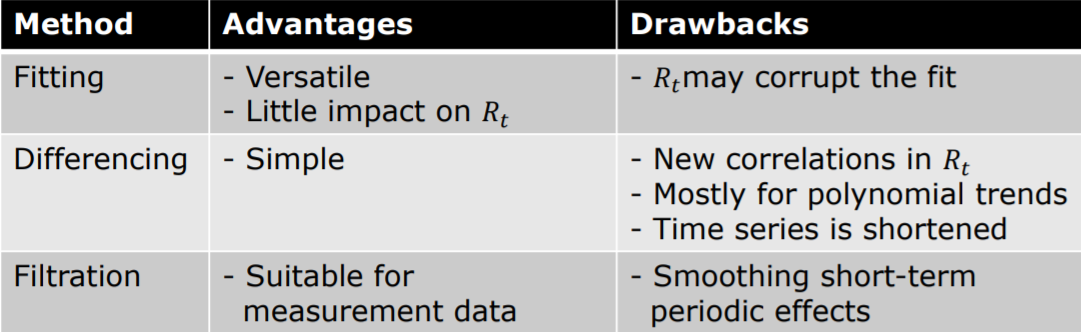
\includegraphics[width=1\linewidth]{adv}

\hypertarget{linear-regression}{%
\subsection{Linear Regression}\label{linear-regression}}

Detrending with linear regression it is possible if the trend is
deterministic (e.g.~a linear trend). You run a linear regression to
estimate the trend and remove it from the data.

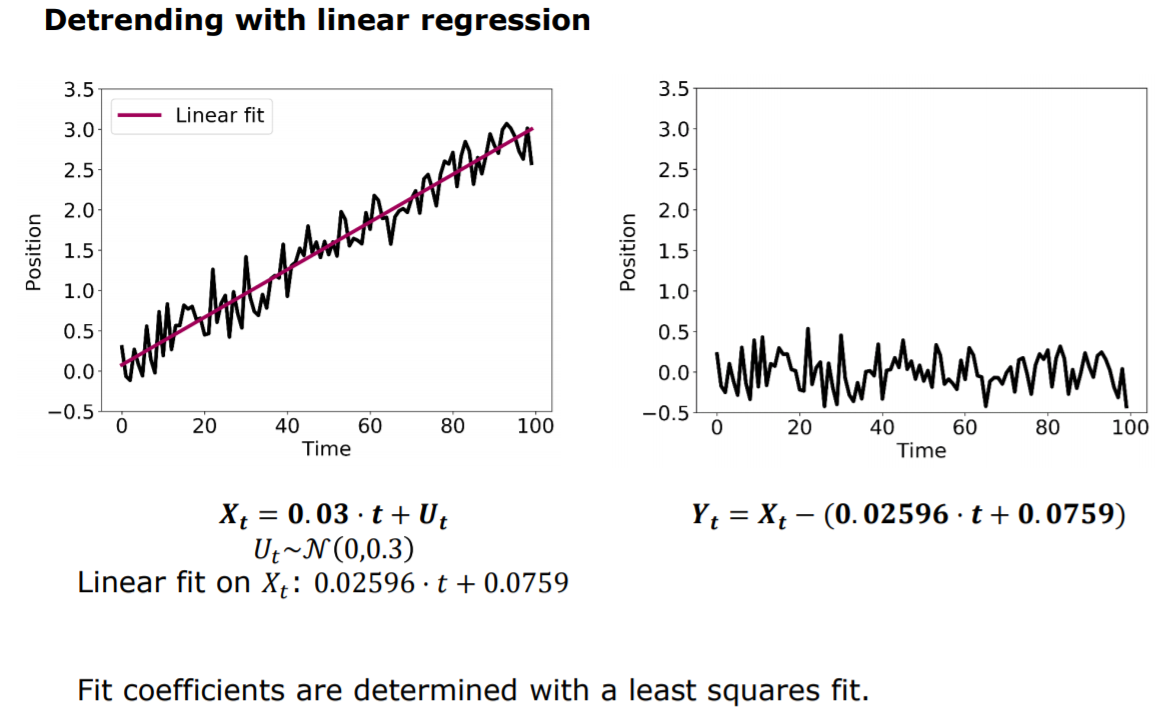
\includegraphics[width=1\linewidth]{detrend}

In deterministic models, the output of the model is fully determined by
the parameter values and the initial conditions.

Stochastic models possess some inherent randomness. The same set of
parameter values and initial conditions will lead to an ensemble of
different outputs.

If the trend is stochastic you should detrend the series by taking first
differences on it.

\hypertarget{differencing}{%
\subsection{Differencing}\label{differencing}}

One way to make a non-stationary time series stationary --- compute the
differences between consecutive observations. Computing the differences
between consecutive observations, is known as differencing.

Differencing can help stabilise the mean of a time series by removing
changes in the level of a time series, and therefore eliminating (or
reducing) trend and seasonality.

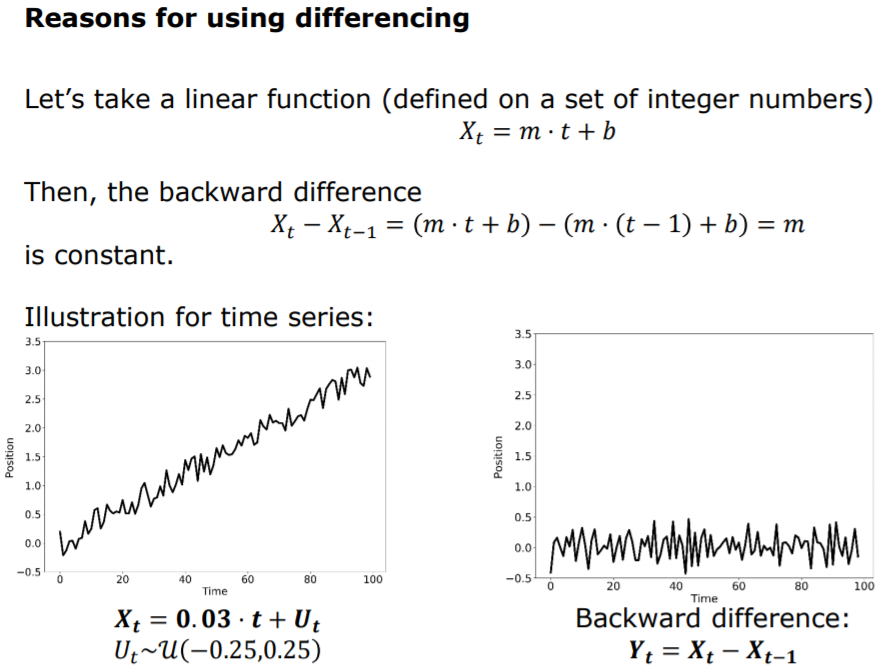
\includegraphics[width=1\linewidth]{rtp_diff}

\textbf{Connection to calculus}

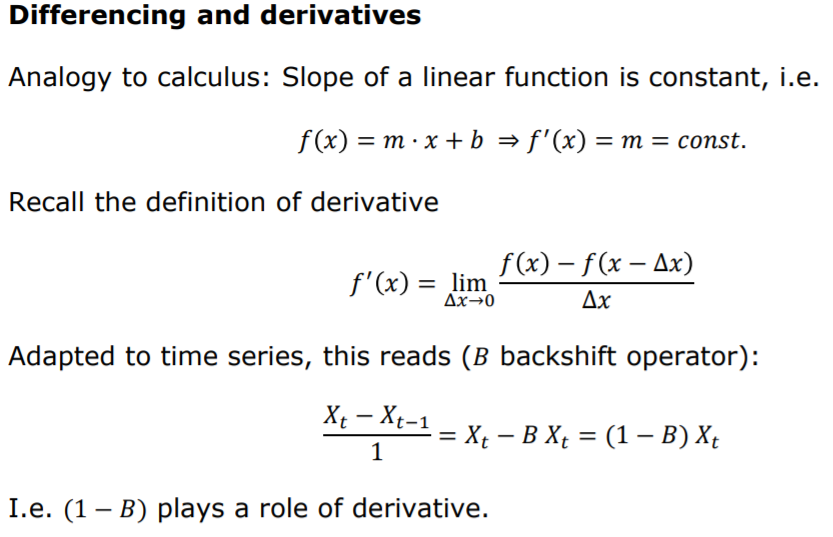
\includegraphics[width=1\linewidth]{derivative}

Summary: + trend and seasonal effect can be removed + procedure is very
quick and very simple to implement

\begin{itemize}
\tightlist
\item
  trend, season and remainder component are NOT known, and cannot be
  visualised
\item
  resulting time series will be shorter than original data set
\item
  differencing creates artificial new dependencies that are different
  from the original ones
\item
  extrapolation of trend, season and remainder is not easily possible
\end{itemize}

\hypertarget{random-walk}{%
\subsection{Random Walk}\label{random-walk}}

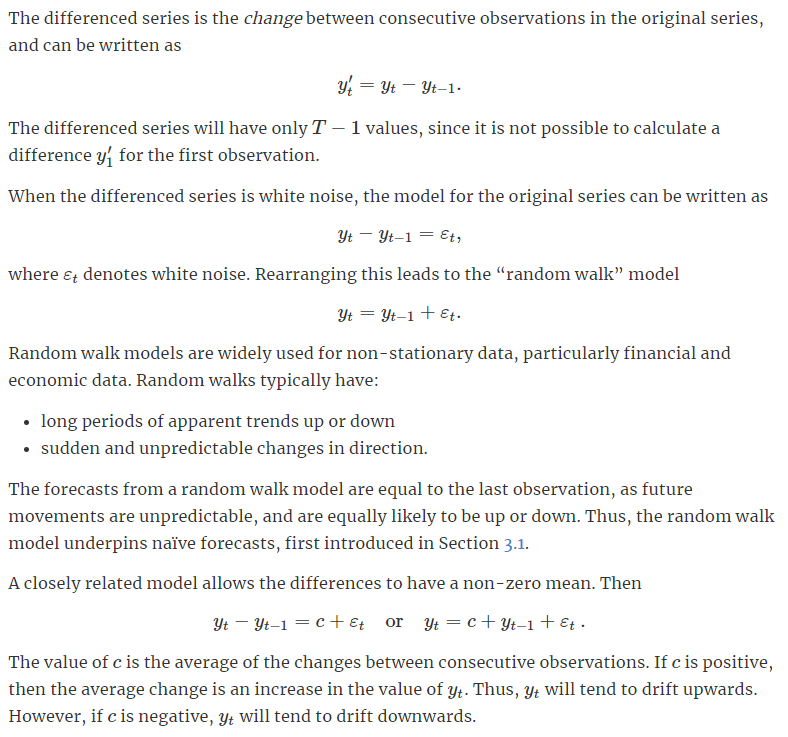
\includegraphics[width=1\linewidth]{random_walk}

\hypertarget{second-order-differencing}{%
\subsection{Second-order differencing}\label{second-order-differencing}}

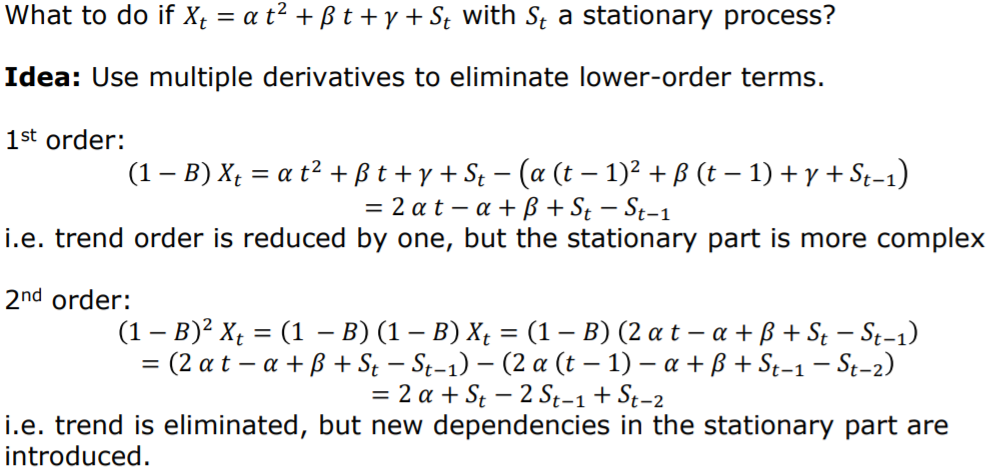
\includegraphics[width=1\linewidth]{2nd_derivative}

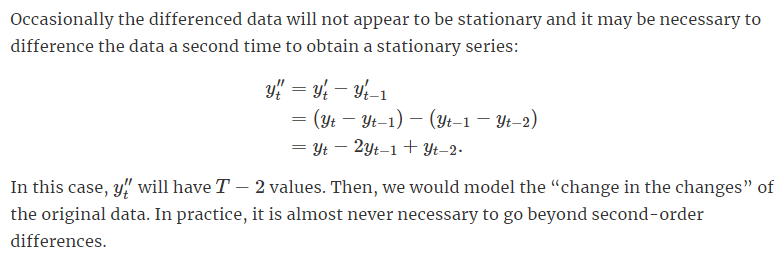
\includegraphics[width=1\linewidth]{diff_2}

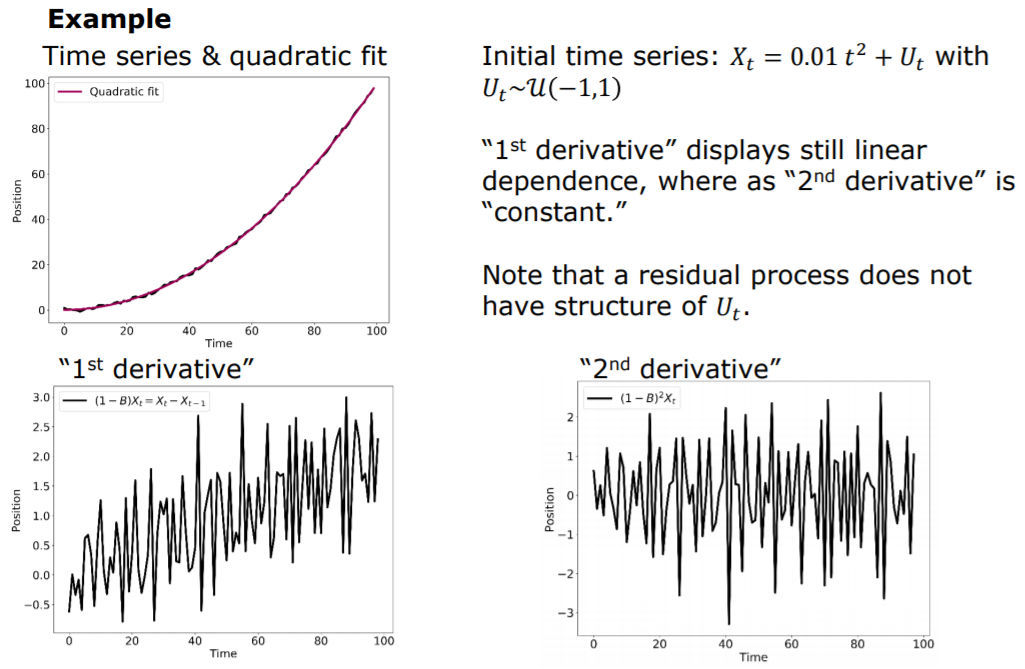
\includegraphics[width=1\linewidth]{2nd}

\hypertarget{taylors-theorem}{%
\subsubsection{Taylor's Theorem}\label{taylors-theorem}}

\begin{Shaded}
\begin{Highlighting}[]
\NormalTok{knitr}\OperatorTok{::}\KeywordTok{include_graphics}\NormalTok{(}\StringTok{'taylor.png'}\NormalTok{)}
\end{Highlighting}
\end{Shaded}

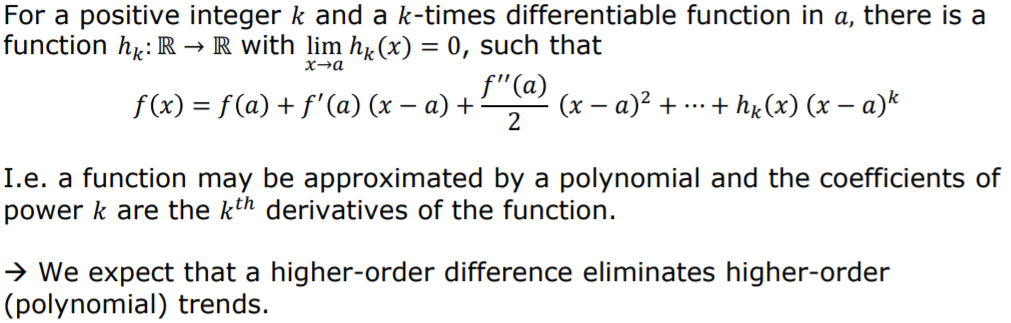
\includegraphics[width=14.04in]{taylor}

\hypertarget{seasonal-differencing}{%
\subsection{Seasonal differencing}\label{seasonal-differencing}}

Seasonality manifests itself by a repetitive behaviour after a fixed lag
time p.

\textbf{Yt = Xt - Xt-p = (1 - B\^{}p)Xt}

Note: (1 - B\^{}p) is NOT (1 - B)\^{}p

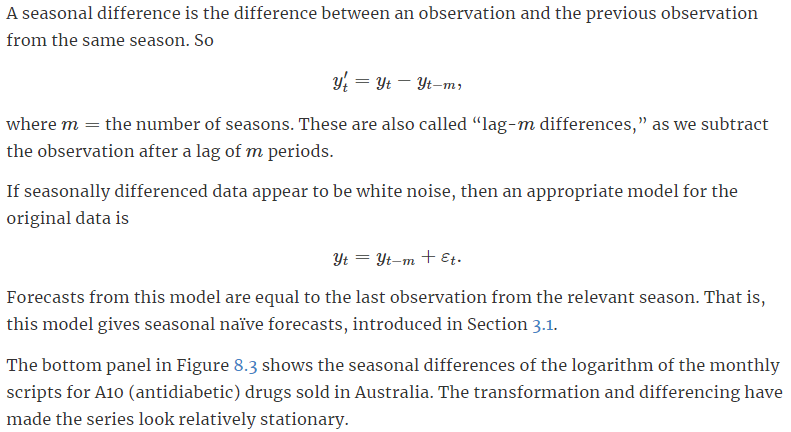
\includegraphics[width=1\linewidth]{deason_diff}

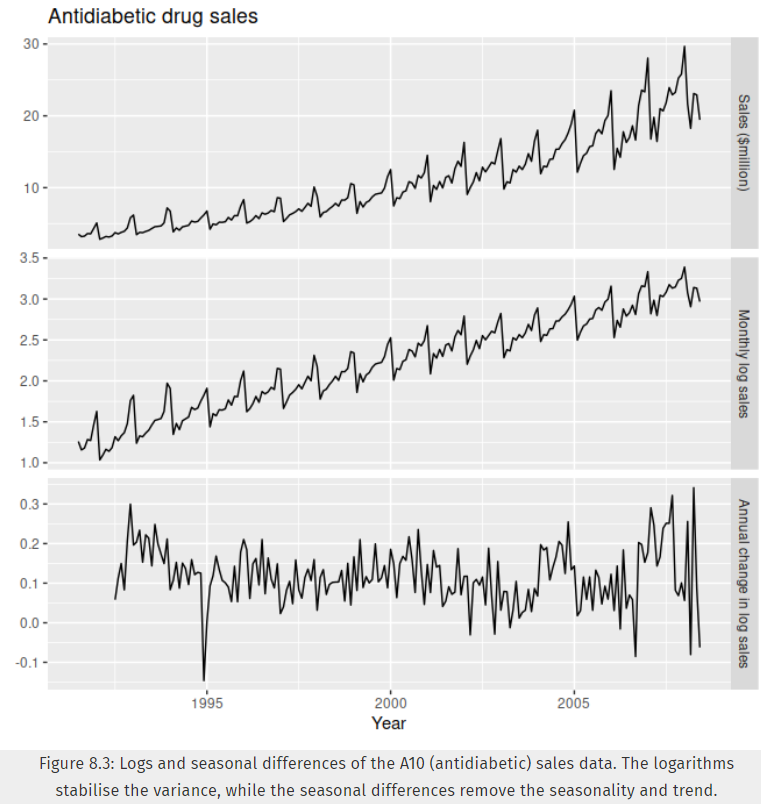
\includegraphics[width=1\linewidth]{drug}

\textbf{Example of time series representation with seasonality}

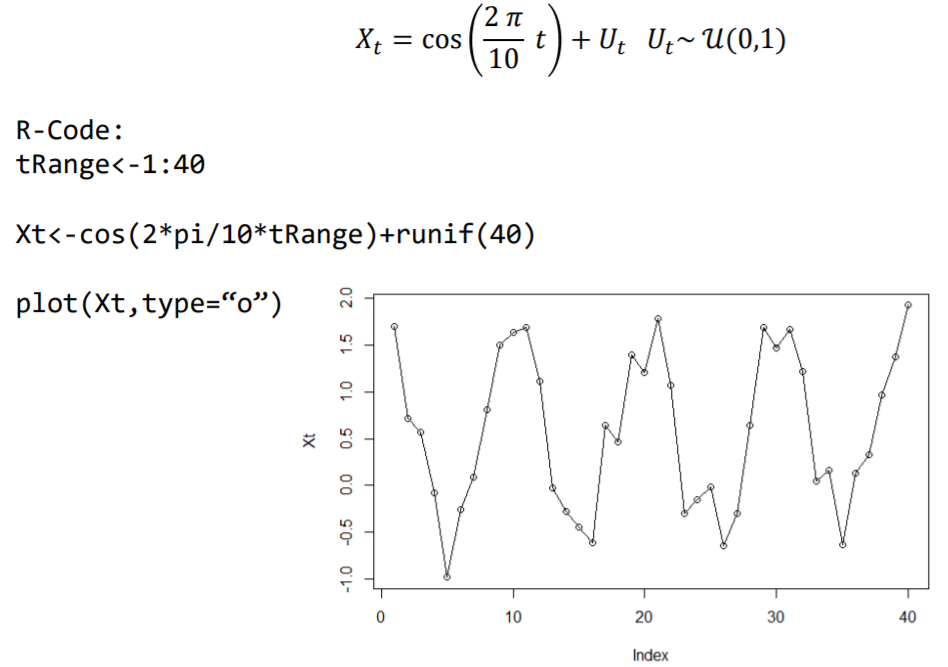
\includegraphics[width=1\linewidth]{cos}

\textbf{Example of time series representation with seasonality}

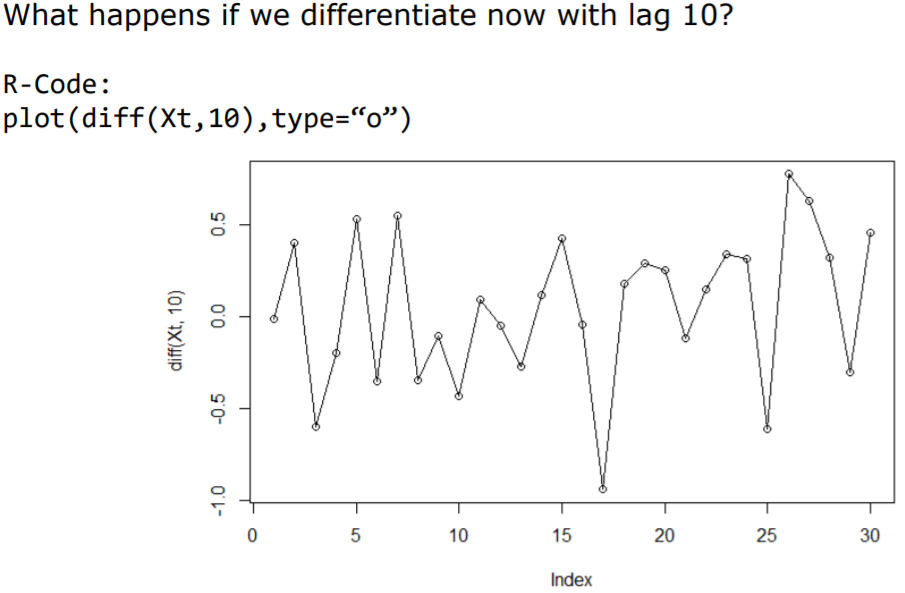
\includegraphics[width=1\linewidth]{cos_diff}

\textbf{Calculation of the time series with seasonality}

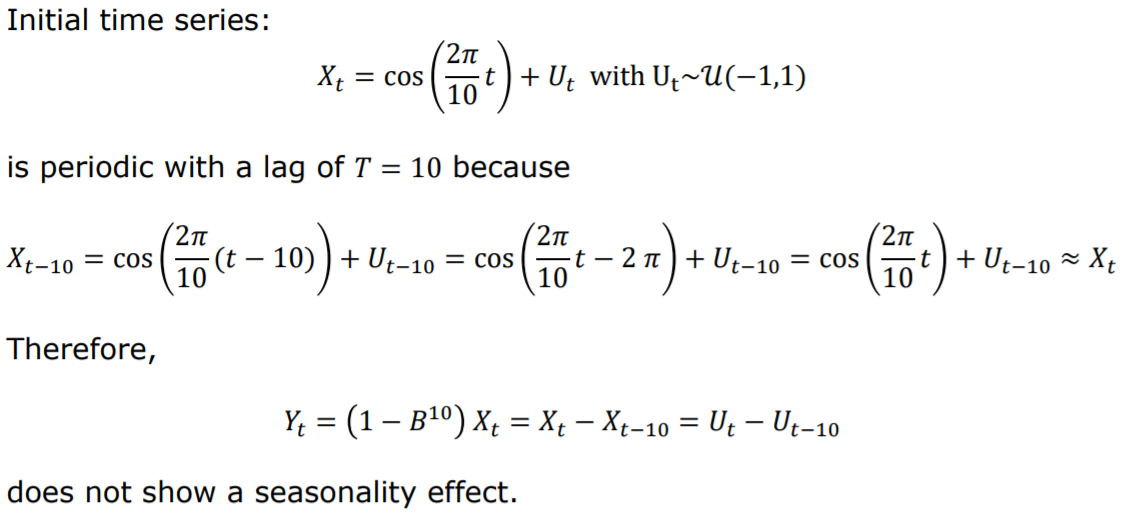
\includegraphics[width=1\linewidth]{calc_cos}

\hypertarget{backshift-operator-and-backshift-notation}{%
\subsection{Backshift operator and Backshift
notation}\label{backshift-operator-and-backshift-notation}}

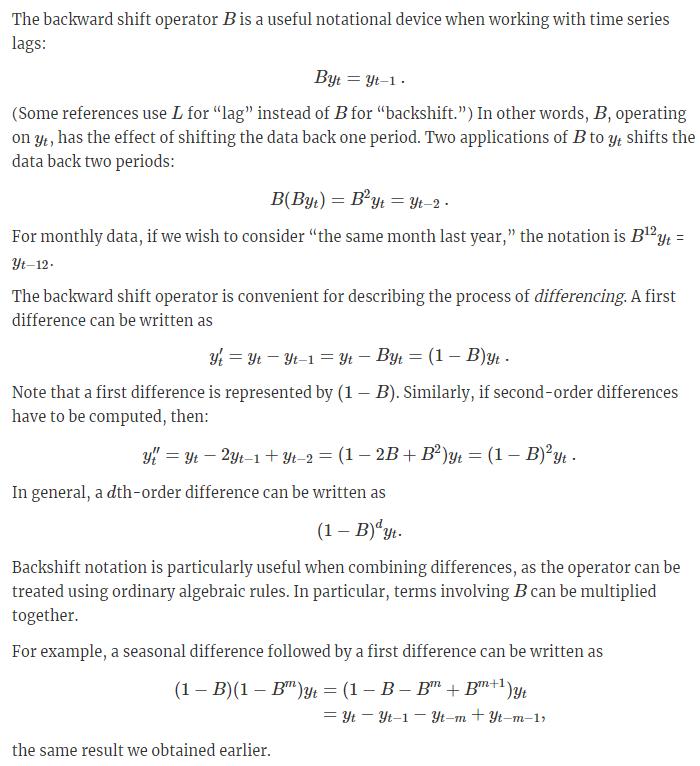
\includegraphics[width=1\linewidth]{backnotation}

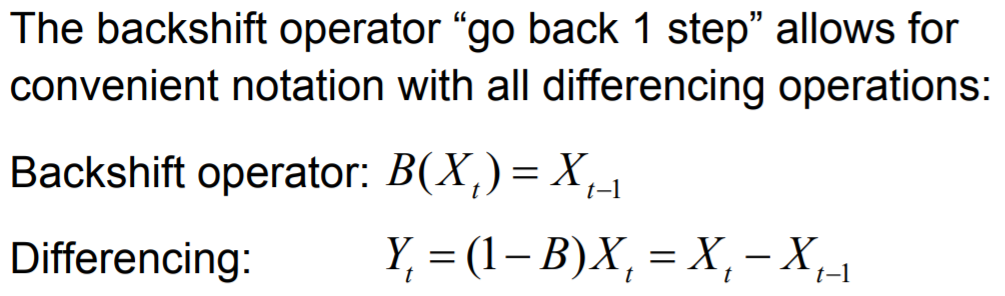
\includegraphics[width=13.96in]{backshift}

\hypertarget{remove-linear-trend-of-a-non-stationary-time-series-by-taking-differences-of-first-order-at-lag-1-diffx-differences-1}{%
\subsubsection{Remove linear Trend of a non-stationary time series by
taking differences of first order at lag 1: diff(x, differences =
1)}\label{remove-linear-trend-of-a-non-stationary-time-series-by-taking-differences-of-first-order-at-lag-1-diffx-differences-1}}

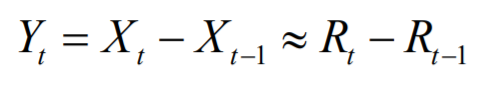
\includegraphics[width=0.5\linewidth]{diff_trend}

The new time series Yt is going to be stationary, but has new, strong
and artificial dependencies

\begin{itemize}
\tightlist
\item
  Yt now are the observation to observation changes in the series, NOT
  longer the observations or remainder itself
\item
  does not yield estimates for trend, season and remainder component
\end{itemize}

\hypertarget{differencing-for-log-transformed-series-difflogx-differences-1-lag-1}{%
\subsubsection{Differencing for log-transformed series: diff(log(x),
differences = 1, lag =
1)}\label{differencing-for-log-transformed-series-difflogx-differences-1-lag-1}}

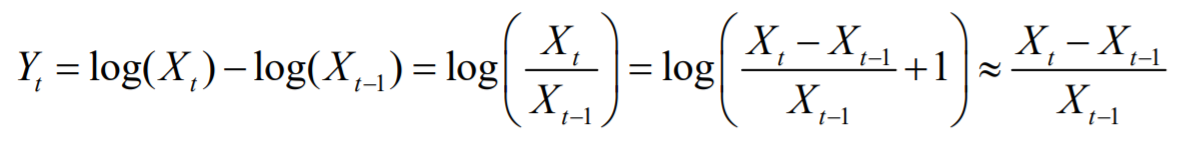
\includegraphics[width=0.5\linewidth]{diff_log}

\hypertarget{remove-polynomial-trend-diffx-differences-2-or-more}{%
\subsubsection{Remove polynomial Trend: diff(x, differences = 2 or
more)}\label{remove-polynomial-trend-diffx-differences-2-or-more}}

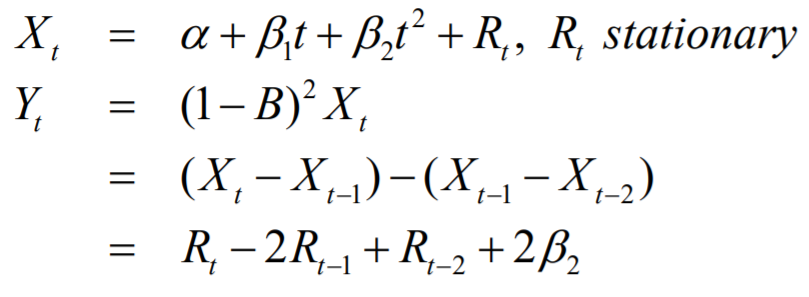
\includegraphics[width=0.5\linewidth]{diff_higher}

This will remove a polynomial trend. A quadratic trend can be removed by
taking second-order differences (differences = 2).

Time series with seasonal effects can be made stationary through
differencing by comparing to the previous periods' value.

\hypertarget{remove-seasonality-diffx-lag-p}{%
\subsubsection{Remove Seasonality: diff(x, lag =
p)}\label{remove-seasonality-diffx-lag-p}}

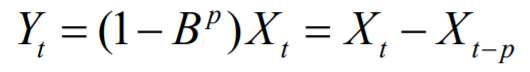
\includegraphics[width=0.5\linewidth]{diff_season}

To remove Trend and Seasonality take first order differences at the lag
= p of the period, which removes both trend and season effects: diff(x,
differences = 1, lag = 12) example: p = 12

\hypertarget{filtration-to-reduce-noise-impact}{%
\subsection{Filtration to reduce noise
impact}\label{filtration-to-reduce-noise-impact}}

Differencing and filtering is not the same!!

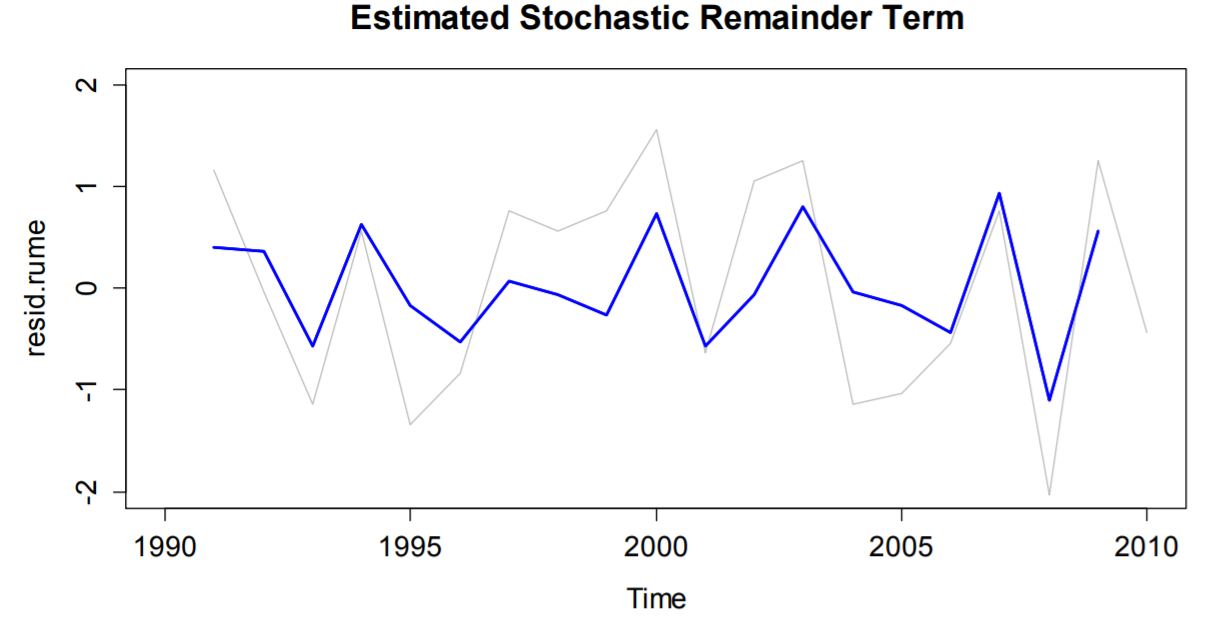
\includegraphics[width=1\linewidth]{diff_filter}

Filtering is used to reduce the noise element, by averaging multiple
(e.g.~3) measurements, short-term variations are smoothed out and the
trend is confirmed -\textgreater{} We obtain a new averaged time series.

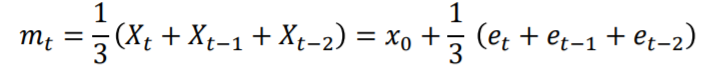
\includegraphics[width=0.25\linewidth]{filt}

In case of seasonality effects, the has to expand over the full period
to extract the trend and to quantify the seasonal impact, the values of
the same time in the season have to be averaged.

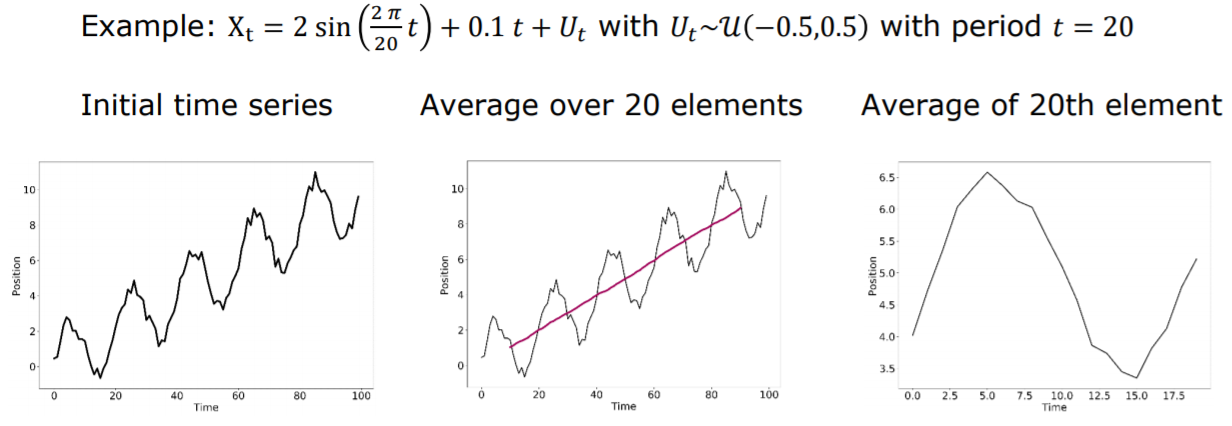
\includegraphics[width=1\linewidth]{avg_season}

\hypertarget{additive-linear-filters}{%
\subsubsection{Additive linear filters}\label{additive-linear-filters}}

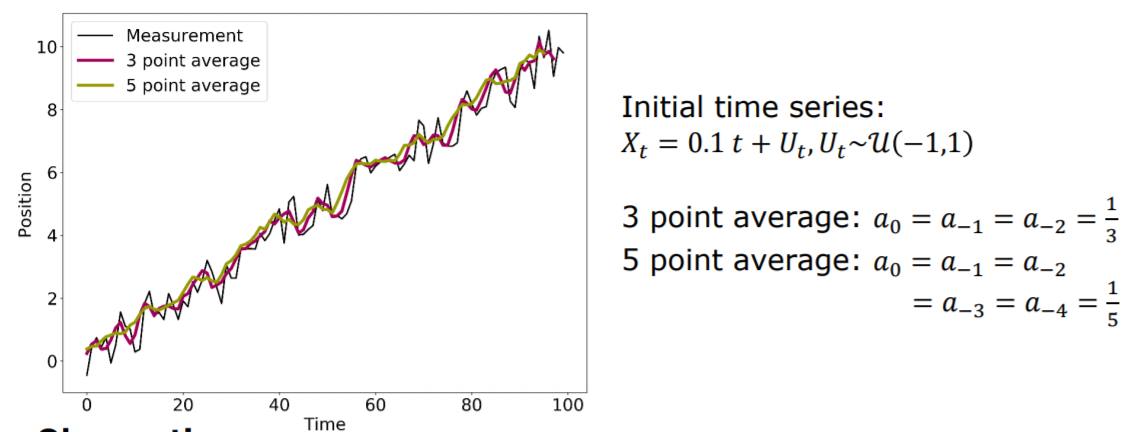
\includegraphics[width=1\linewidth]{avg}

\textbf{Example of filter aplication}

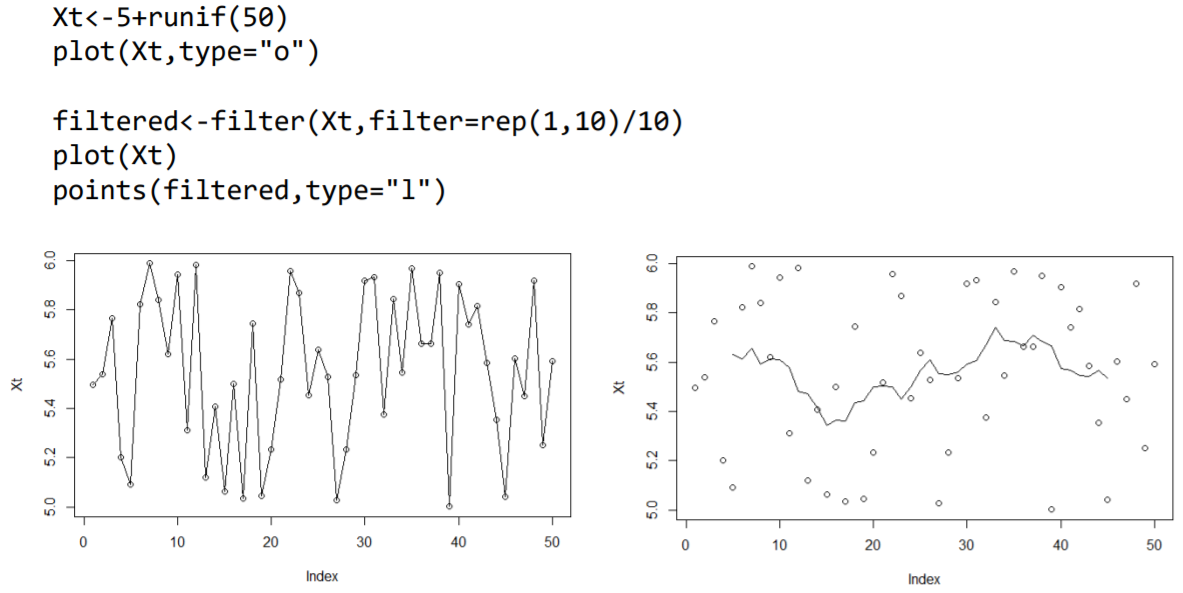
\includegraphics[width=1\linewidth]{filter_ex}

\hypertarget{exponential-smoothing-filter}{%
\subsubsection{Exponential smoothing
filter}\label{exponential-smoothing-filter}}

\hypertarget{advantages-and-drawbacks}{%
\subsubsection{Advantages and
Drawbacks}\label{advantages-and-drawbacks}}

Soomthing, filtering:

\begin{itemize}
\item
  trend and seasonal effect can be estimated
\item
  trend, season and remainder are explicitly known \& can be visualized
\item
  procedure is transparent and simple to implement
\item
  resulting time series will be shorter than the original
\item
  the running mean is not the very best smoother
\item
  extraolation of trend and season are not entirely obvious
\item
  seasonal effect is handled as constant over time
\end{itemize}

\hypertarget{decomposition}{%
\subsection{Decomposition}\label{decomposition}}

The aim of time series analysis is to reduce the series to stationarity.

\hypertarget{basic-structures}{%
\subsubsection{Basic Structures}\label{basic-structures}}

The following two structures are considered for basic decomposition
models: Additive: Xt = Trend + Seasonal + Random Multiplicative: Xt =
Trend * Seasonal * Random

\textbf{How to Choose Between Additive and Multiplicative
Decompositions} - The additive model is useful when the seasonal
variation is relatively constant over time. - The multiplicative model
is useful when the seasonal variation increases over time.

The additive decomposition is the most appropriate if the magnitude of
the seasonal fluctuations, or the variation around the trend-cycle, does
not vary with the level of the time series.

When the variation in the seasonal pattern, or the variation around the
trend-cycle, appears to be proportional to the level of the time series,
then a multiplicative decomposition is more appropriate. Multiplicative
decompositions are common with economic time series.

An alternative to using a multiplicative decomposition is to first
transform the data until the variation in the series appears to be
stable over time, then use an additive decomposition. When a log
transformation has been used, this is equivalent to using a
multiplicative decomposition because:

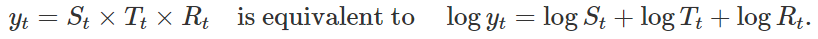
\includegraphics[width=1\linewidth]{components}

\hypertarget{identify-characteristics-of-time-series}{%
\subsection{Identify characteristics of Time
Series}\label{identify-characteristics-of-time-series}}

Have a look at the following set of time series. For every series,
shortly answer the following questions (motivate your answers): • Is the
time series stationary? • Is there a trend? • Can one find some seasonal
effect? If yes, what is the period? • Which transformation should be
applied (if required)?

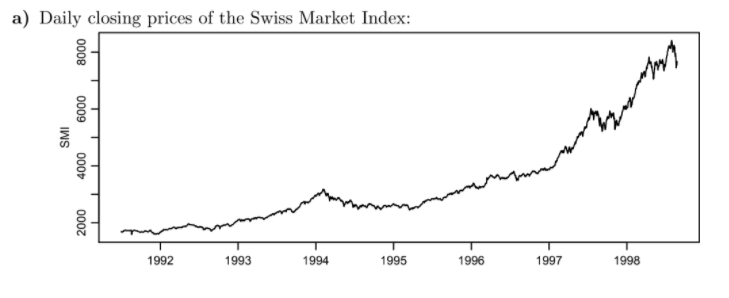
\includegraphics[width=1\linewidth]{Ex1.3a}

Answer: - non stationary - non linear trend, mostly increasing - no
seasonal component - log transformation

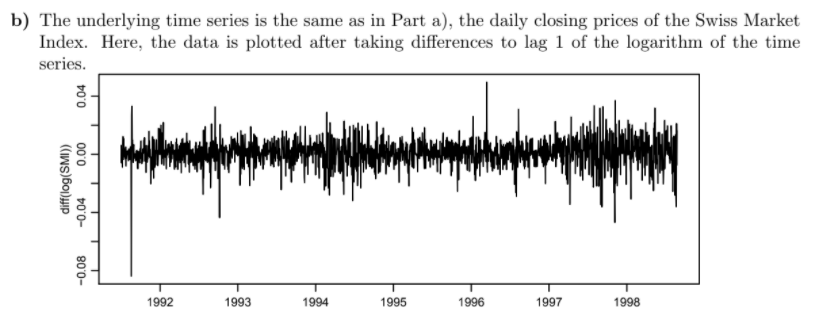
\includegraphics[width=1\linewidth]{Ex1.3b}

Answer: - seems stationary - trend from before was removed by
diff(difference = 1) - constant variance achieved by taking the
logarithm. However Log-Returns are NOT stationary, because of volatility
clusters

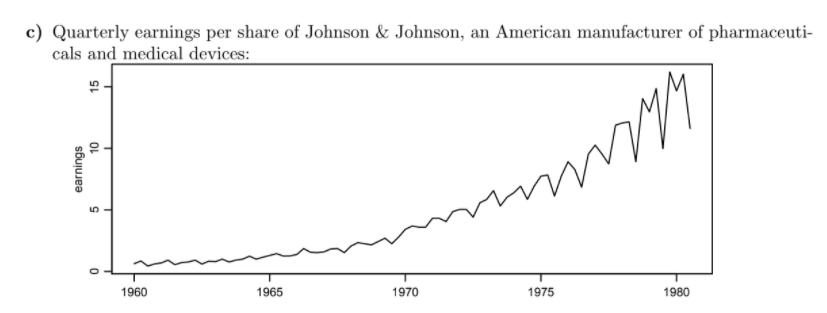
\includegraphics[width=1\linewidth]{Ex1.3c}

Answer: - non stationary - exponential increasing trend - seasonal
component with period 1 year - increasing variance, log transformation
benefitial to get additive components

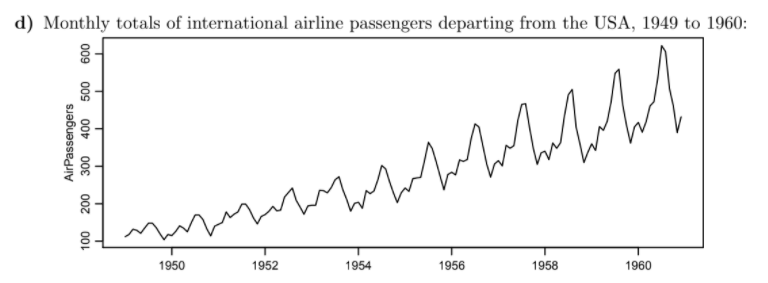
\includegraphics[width=1\linewidth]{Ex1.3d}

Answer: - non stationary - increasing trend - seasonal component with
period 1 year and increasing variance - increasing variance, log
transformation benefitial to get additibe components

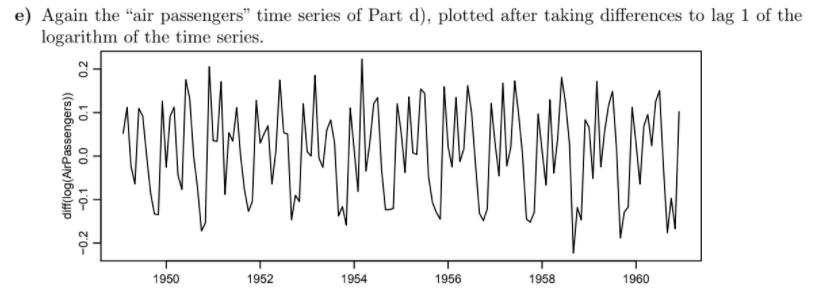
\includegraphics[width=1\linewidth]{Ex1.3e}

Answer: - non stationary - no visible trend - seasonal effect with
period 1 year

Yeary numbers of sunspots:

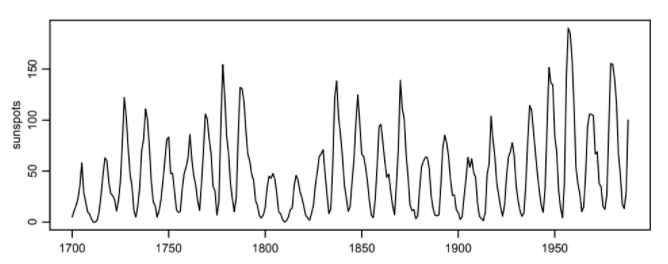
\includegraphics[width=1\linewidth]{Ex1.3f}

Answer: - likely to be stationary - no trend - no seasonal effect -
periodicity with period of 11 years - variance maybe different over time
- log transformation required due to right skewness

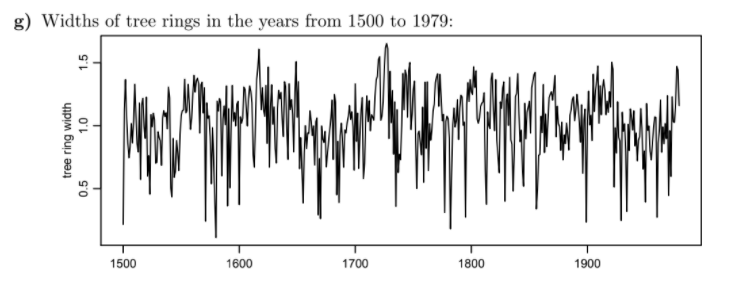
\includegraphics[width=1\linewidth]{Ex1.3g}

Answer: - probably stationary - no clear trend visible - no seasonal
effect visible - no transformation required

\hypertarget{quantitative-description-and-correlation-functions}{%
\section{Quantitative Description and Correlation
functions}\label{quantitative-description-and-correlation-functions}}

Autocorrelation measures the linear relationship between lagged values
of a time series and quantifies dependencies. There are several
autocorrelation coefficients, corresponding to each panel in the lag
plot. For example,\\
r1 measures the relationship between yt and yt−1, r2 measures the
relationship between yt and yt−2, and so on.

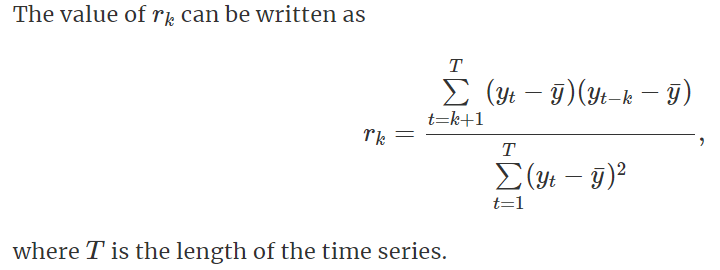
\includegraphics[width=0.5\linewidth]{auto}

\hypertarget{what-is-important-about-acf-estimation}{%
\subsection{What is important about ACF
estimation?}\label{what-is-important-about-acf-estimation}}

\begin{itemize}
\tightlist
\item
  Correlations are never to be trusted without a visual inspection with
  a scatterplot.
\item
  The bigger the lag k, the fewer data pairs remain for estimating the
  acf at lag k.
\item
  Rule of the thumb: the acf is only meaningful up to about
\end{itemize}

\begin{enumerate}
\def\labelenumi{\alph{enumi})}
\tightlist
\item
  lag 10*log10(n)
\item
  lag n/4
\end{enumerate}

\begin{itemize}
\tightlist
\item
  The estimated sample ACs can be highly correlated. \textbf{- The
  correlogram is only meaningful for stationary series!!!}
\end{itemize}

\hypertarget{lagged-scatterplots}{%
\subsection{Lagged Scatterplots}\label{lagged-scatterplots}}

With lagged scatterplots correlations of consecutive observations are
possible. Original time series values will be plotted against a
time-shifted version. e.g.~xi, xi-k. The average over a realization will
be exchanged with the average over time. We assume that for stationary
time series, the correlation depends only on the lag.

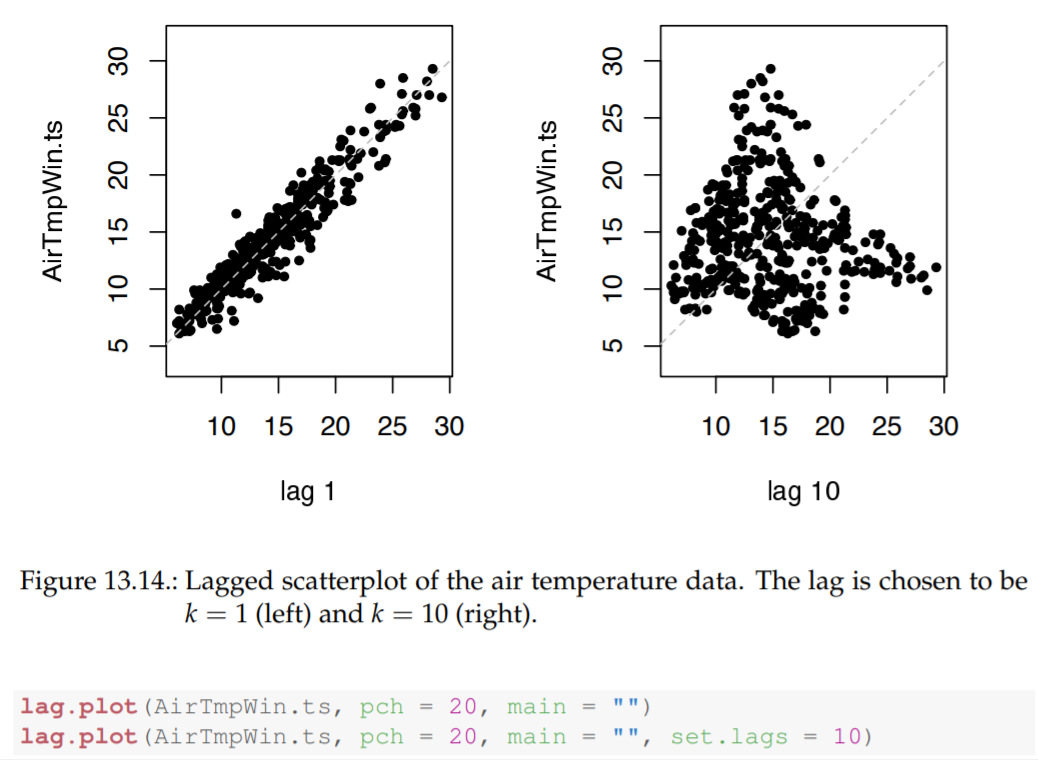
\includegraphics[width=1\linewidth]{lagplot}

Observations:

The plot with lag 1 shows a inear pattern, which indicates a correlation
between subsequent data points. A ag 10 however results in a rather
unspecific scatter plot.

Formula:

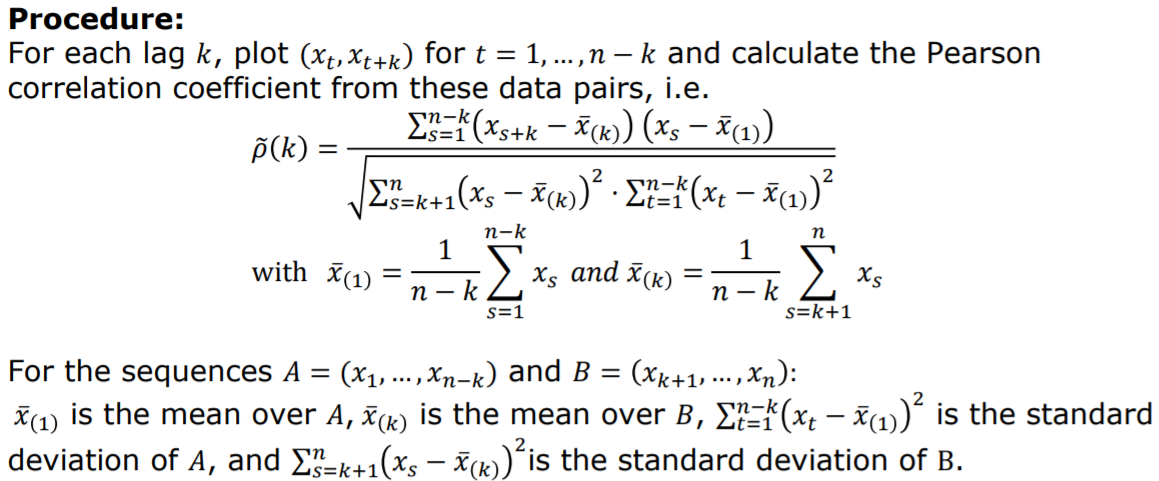
\includegraphics[width=1\linewidth]{lag}

Outliers may be diagnosed by lagged scatter plots. Note that each
outlier causes other outliers.

Strategies for coping with outliers: a) Delete the point or replace it
with Na (most functions in R can handle this)

Replace the outlier value with b) global mean of the series c) nearest
value in the vicinity d) local mean of the series (i.e.~odd number of
surrounding values) e) fit a time series model to the
remaining/surrounding values and predict the missing value

\hypertarget{plug-in-estimator}{%
\subsection{Plug-in Estimator}\label{plug-in-estimator}}

Plug-in estimation is the standard approach for computing
autocorrelations in time series analysis. It is better than the lagged
scatterplot idea, however the plug-in estimator p(k) is sensitive to
outliers.

\textbf{Calculated with the acf() function in R.}

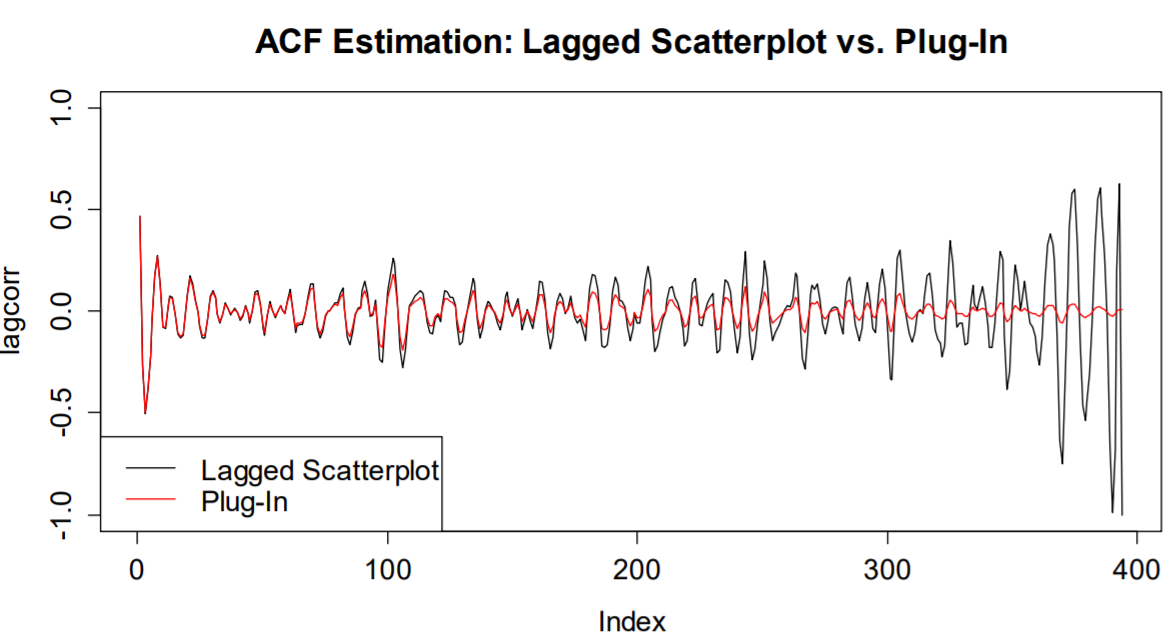
\includegraphics[width=1\linewidth]{comp}

\textbf{Formula}

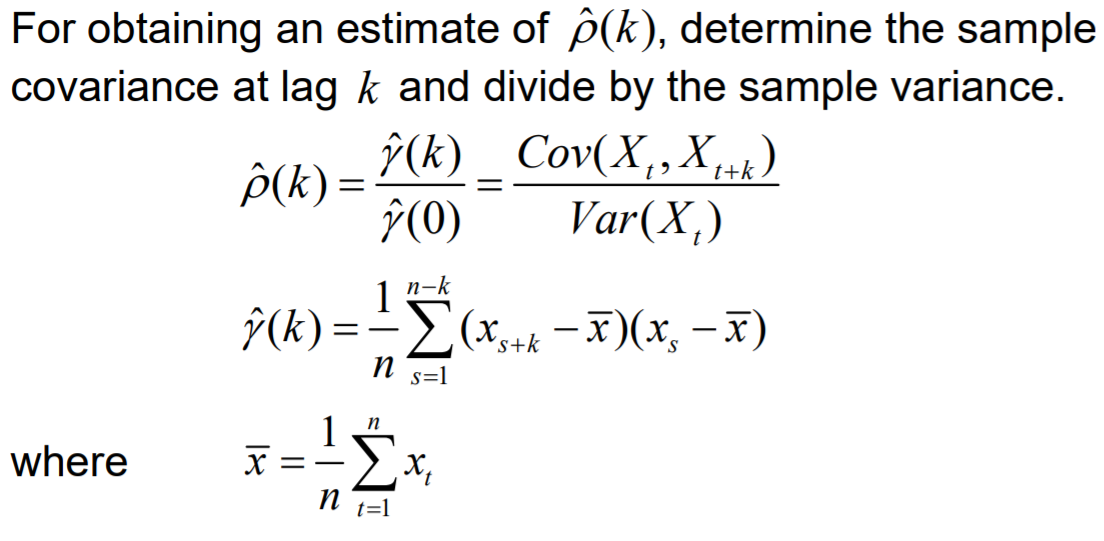
\includegraphics[width=1\linewidth]{plugin}

\hypertarget{lagged-scatterplot-estimator-versus-plug-in-estimator-for-autocorrelation}{%
\subsubsection{Lagged scatterplot estimator versus Plug-in estimator for
autocorrelation}\label{lagged-scatterplot-estimator-versus-plug-in-estimator-for-autocorrelation}}

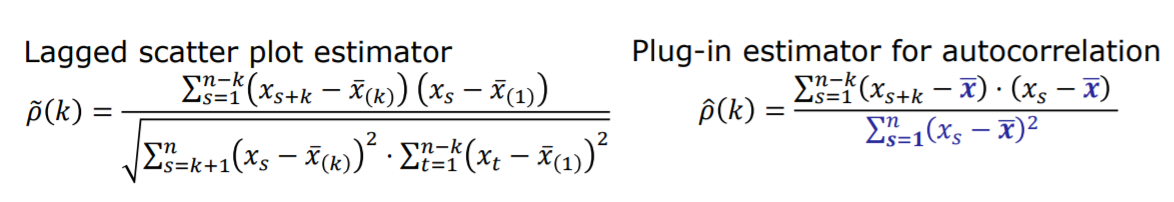
\includegraphics[width=1\linewidth]{lag_plug}

\hypertarget{autocorrelation-acf}{%
\subsection{Autocorrelation ACF}\label{autocorrelation-acf}}

The ACF plot is also useful for identifying non-stationary time series.
For a stationary time series, the ACF will drop to zero relatively
quickly, while the ACF of non-stationary data decreases slowly. Also,
for non-stationary data, the value of r1 is often large and positive.

\begin{itemize}
\tightlist
\item
  For time series shorter than 100 elements, the plug-in estimator p(k)
  is biased
\end{itemize}

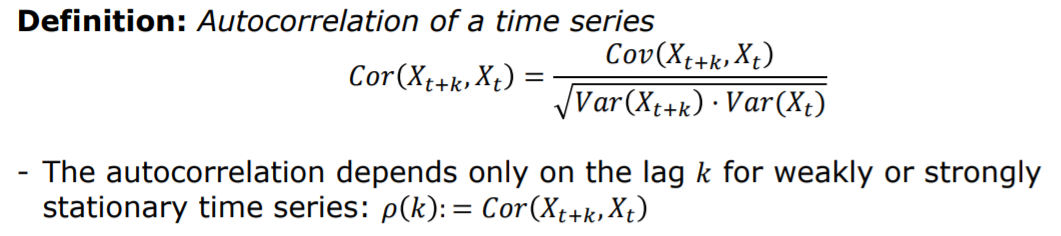
\includegraphics[width=1\linewidth]{cor}

Concept: The correlation p(k)\^{}2 squared corresponds to the percentage
of variability explained by the linear association between Xt and Xt+k
-\textgreater{} R\^{}2.

\textbf{Variance: Var(Xt) = E{[}(Xt-mean)\^{}2{]} = Cov(Xt,Xt) with mean
= E{[}Xt{]}}

\hypertarget{acf-characteristics}{%
\subsubsection{ACF Characteristics}\label{acf-characteristics}}

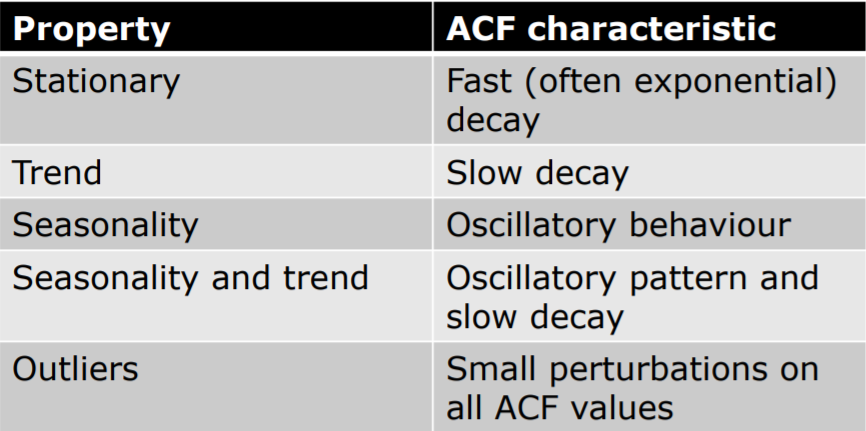
\includegraphics[width=1\linewidth]{acf}

\hypertarget{patterns-in-acf-of-non-stationary-time-series}{%
\subsubsection{Patterns in ACF of non-stationary time
series}\label{patterns-in-acf-of-non-stationary-time-series}}

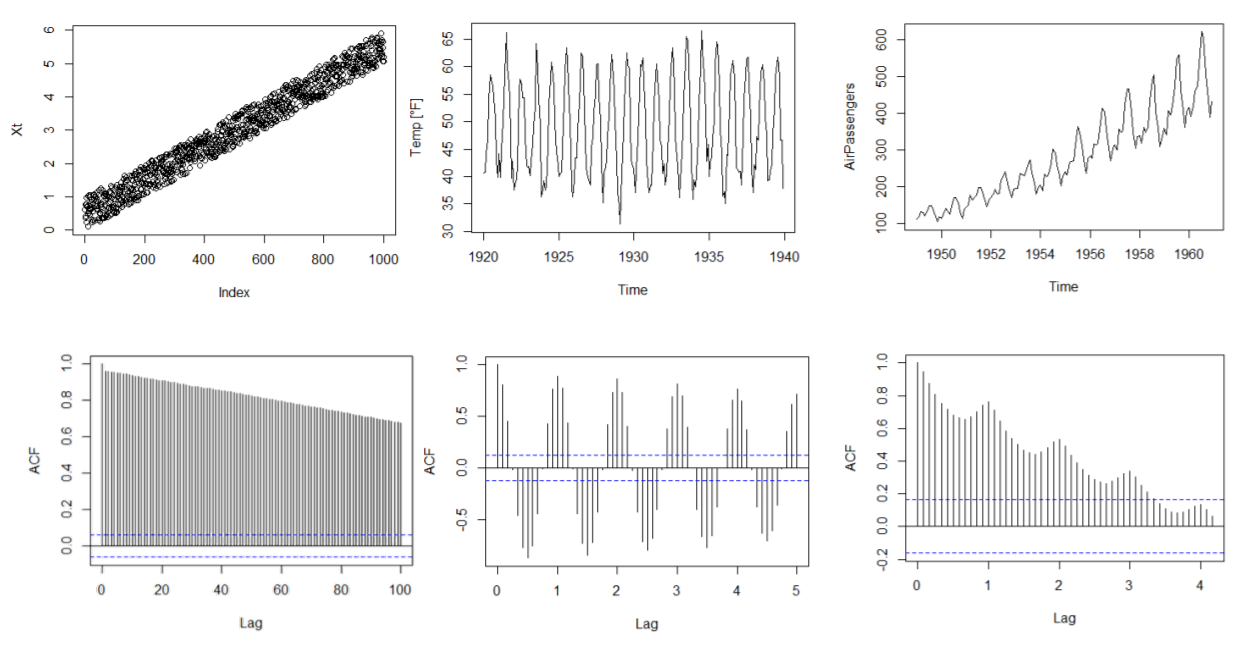
\includegraphics[width=1\linewidth]{patt}

\hypertarget{trend-in-acf-plots}{%
\subsubsection{Trend in ACF plots}\label{trend-in-acf-plots}}

When data have a trend, the autocorrelations for small lags tend to be
large and positive because observations nearby in time are also nearby
in size. So the ACF of trended time series tend to have positive values
that slowly decrease as the lags increase.

\hypertarget{season-in-acf-plots}{%
\subsubsection{Season in ACF plots}\label{season-in-acf-plots}}

When data are seasonal, the autocorrelations will be larger for the
seasonal lags (at multiples of the seasonal frequency) than for other
lags.

When data are both trended and seasonal, you see a combination of these
effects.

\hypertarget{partial-autocorrelation-pacf}{%
\subsection{Partial Autocorrelation
PACF}\label{partial-autocorrelation-pacf}}

The ACF measures the „simple`` dependence between and , whereas the PACF
measures that dependence in a „multiple`` fashion. Given a time series ,
the partial autocorrelation of lag , is the autocorrelation between and
with the linear dependence of through to removed. It is a conditional
correlation of the random variables A, B under condition C.

\hypertarget{ljung-box-test}{%
\subsection{Ljung-Box Test}\label{ljung-box-test}}

The Ljung-Box approach tests the Null-Hypothesis that a number of
autocorrelation coefficients are simultaneously equal to 0. Meaning, the
Ljung-Box test tests for significant autocorrelation in a time series.

The Ljung--Box test may be defined as:

H0: The data are independently distributed (p-value \textgreater{} 0.05)

Ha: The data are not independently distributed; they exhibit serial
correlation. (p-value \textless{} 0.05)

Formula and R-code:

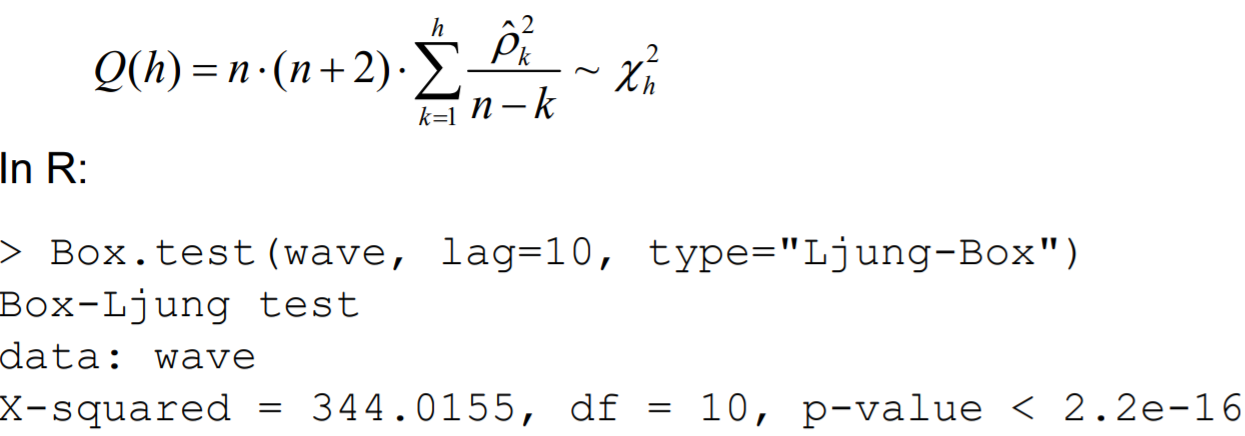
\includegraphics[width=1\linewidth]{ljung}

Outcome:

The p-value shows that the series is not independently distributed. H0
rejected. Ha accepted.

\hypertarget{white-noise}{%
\subsection{White Noise}\label{white-noise}}

Time series that show no autocorrelation are called white noise. For
white noise series, we expect each autocorrelation to be close to zero.
Of course, they will not be exactly equal to zero as there is some
random variation. For a white noise series, we expect 95\% of the spikes
in the ACF to lie within ±2/√T where T is the length of the time series.
It is common to plot these bounds on a graph of the ACF. If one or more
large spikes are outside these bounds, or if substantially more than 5\%
of spikes are outside these bounds, then the series is probably not
white noise.

\hypertarget{stl-decomposition}{%
\subsection{STL Decomposition}\label{stl-decomposition}}

The Seasonal-Trend Decomposition Procedure by Loess • is an iterative,
non-parametric smoothing algorithm • yields a simultaneous estimation of
trend and seasonal effect -\textgreater{} robust! + very simple to apply
+ very illustrative and quick + seasonal effect can be constant or
smoothly varying - model free, extrapolation and forecasting is
difficult

-\textgreater{} Good method for „having a quick look at the data``

\hypertarget{linear-modeling-with-ar-ma-and-arma}{%
\section{Linear Modeling with AR, MA and
ARMA}\label{linear-modeling-with-ar-ma-and-arma}}

Exponential smoothing and ARIMA models are the two most widely used
approaches to time series forecasting, and provide complementary
approaches to the problem. While exponential smoothing models are based
on a description of the trend and seasonality in the data, ARIMA models
aim to describe the autocorrelations in the data.

Steps: - remove trend - remove seasonality - fit residuals

Purpose of modelling: - to explain hidden structures - to predict future
values

Challenge: - What model is the most suitable model?

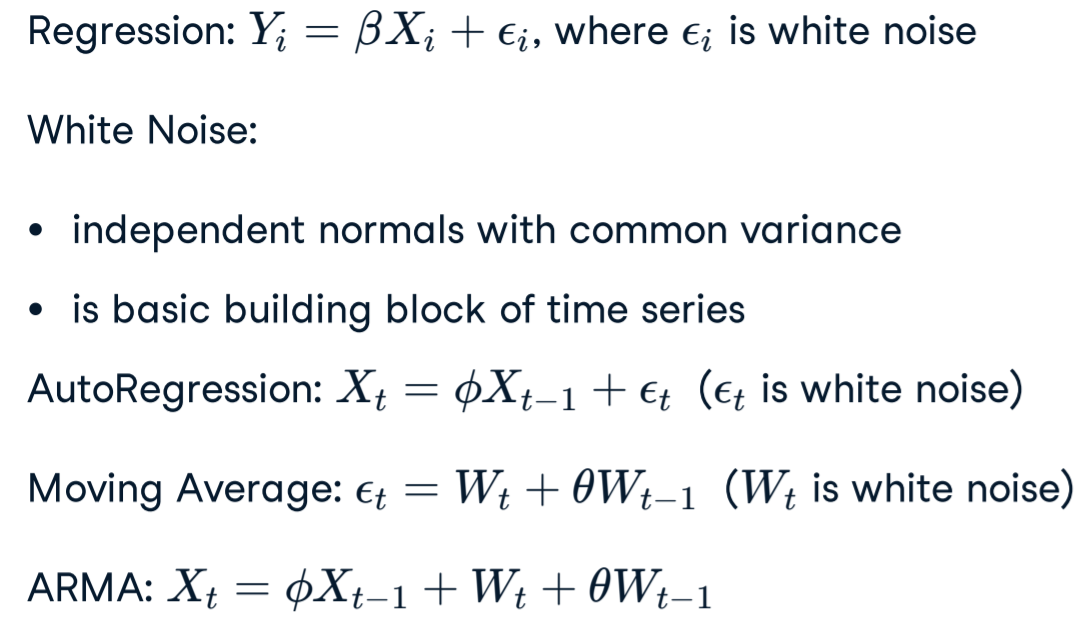
\includegraphics[width=1\linewidth]{model}

\hypertarget{arima-models-overview}{%
\subsection{ARIMA models: Overview}\label{arima-models-overview}}

\includegraphics[width=0.5\linewidth]{over}

\includegraphics[width=1\linewidth]{arima} \#\# Simulating data

\hypertarget{simulating-an-arp-model}{%
\subsubsection{Simulating an AR(p)
model}\label{simulating-an-arp-model}}

R-code: arima.sim(n=1000, list(ar=c(alpha1, alpha2,\ldots,alpha(p))))

\hypertarget{simulating-a-maq-model}{%
\subsubsection{Simulating a MA(q) model}\label{simulating-a-maq-model}}

R-code: arima.sim(n = 1000, list(ma=c(beta1, beta2,\ldots,beta(q))))

\hypertarget{simulating-an-armapq-model}{%
\subsubsection{Simulating an ARMA(p,q)
model}\label{simulating-an-armapq-model}}

R-code: arima.sim(n = 1000, list(ar=c(alpha1,
alpha2,\ldots,alpha(p)),ma=c(beta1, beta2,\ldots,beta(q))))

\hypertarget{theoretical-autocorrelation-function}{%
\subsubsection{Theoretical autocorrelation
function}\label{theoretical-autocorrelation-function}}

R-code: ARMAacf(ar=c(alpha1,alpha2,\ldots,alpha(p)), pacf=TRUE) R-code:
ARNAacf(ma=c(beta1,beta2,\ldots,beta(q)), pacf= TRUE)

\hypertarget{characteristic-polynomial}{%
\subsection{Characteristic polynomial}\label{characteristic-polynomial}}

\includegraphics[width=0.75\linewidth]{poly}

\hypertarget{arp---autoregressive-models}{%
\subsection{AR(p) - Autoregressive
Models}\label{arp---autoregressive-models}}

AR Models are exclusively used for the modeling of STATIONARY processes
and base on the idea that the current value of the series can be
explained by a linear combination of the p previous values **Xt-p + et
(et = innovation = `completely independent term'). Meaning, we forecast
the variable of interest using a linear combination of past values of
the variable. The term autoregression indicates that it is a regression
of the variable against itself.

\includegraphics[width=0.5\linewidth]{ar}

For a AR(1) process its definition it's:

\includegraphics[width=0.25\linewidth]{arp1}

That means that the random walk is a special case of an AR(1) with a1 =
1.

An AR(p) stochastic process is weakly stationary, if all complex roots
of the characteristic polynomial exceed 1 in absolute value.

R-Code: polyroot() function -\textgreater{} computes the complex roots
of a given polynomial.

Changing the parameters ϕ1,\ldots,ϕp results in different time series
patterns.

\includegraphics[width=0.5\linewidth]{ar1}

\hypertarget{fitting-arp-models}{%
\subsubsection{Fitting AR(p)-Models}\label{fitting-arp-models}}

\textbf{1) Model identification and order identification} - is an AR
process suitable, and what is the p? - will be based on
ACF/PACF-Analysis (ACF fast decaying/PACF cut-off at p) - order
identification (cut-off of PACF)

\includegraphics[width=1\linewidth]{ident}

\textbf{2) Parameter Estimation and Fitting} - Regression approach with
OLS - Yule-Walker-Equations - MLE - Burg-Algorithm

\textbf{3) Model Diagnostic -\textgreater{} Residual Analysis} - Time
Series plot of Êt (Êt = Residuals) - ACF/PACF plot of Êt (Êt =
Residuals) - QQ-plot of Êt (Êt = Residuals)
-\textgreater\textgreater\textgreater{} the innovation time series Êt
should look like White Noise - simulation of time series and qualitative
comparison

\#\#\#1) Autocorrelation of AR(p) processes

Autocorrelation function is used to clarify if the AR(p) model is the
right choice and what is the proper order p for the given data, but it
will turn out that the ACF is not sufficient, while we need to use the
\textbf{partial autocorrelation}.

\#\#2) Parameter identification

The following methods are equal for theoretical models and yield similar
results on realizations. The models are sensitive to outliers and work
best on data that follows a normal (gaussian) distribution.

\hypertarget{ols---ordinary-least-square}{%
\subsubsection{OLS - Ordinary Least
Square}\label{ols---ordinary-least-square}}

Procedure: 1) estimate the global mean and determine xt = yt - m 2)
carry out regression on xt without intercept; resulting parameters are
a1, a2, \ldots{} , a(p) 3) estimate the standard deviation (sd) of the
innovation from the standard deviation of the residual

R-code: ar.ols(data, order = p)

\hypertarget{yule-walker-equations}{%
\subsubsection{Yule Walker Equations}\label{yule-walker-equations}}

These equations are used for fitting an AR(p)-model:

\begin{enumerate}
\def\labelenumi{\arabic{enumi})}
\tightlist
\item
  estimate the ACF from a time series
\item
  plug-in the estimates into the Yule-Walker-Equations
\item
  the solution are the AR(p)-coefficients
\end{enumerate}

Note: the model coefficients and the ACF values are interlaced

R-code: ar.yw(data, order = p)

\hypertarget{burg-equations-algorithm}{%
\subsubsection{Burg' Equation's
Algorithm}\label{burg-equations-algorithm}}

Another fitting cost function that exploit (erschliessen) the first p
function values.

R-code: ar.burg(data, order.max=p)

\hypertarget{mle---maximum-likelihood-estimator}{%
\subsubsection{MLE - Maximum Likelihood
Estimator}\label{mle---maximum-likelihood-estimator}}

Determines the parameter based on an optimization of the maximum
likelihood function. This requires the choice of a probability model for
the time series.

R-code: arima(data, order=c(2,0,0))

-\textgreater\textgreater\textgreater\textgreater{} All estimation
methods mentioned above yield similar results.

\textbf{How to choose the optimum model order p?}

\hypertarget{aic---akaike-information-criterion}{%
\subsubsection{AIC - Akaike Information
Criterion}\label{aic---akaike-information-criterion}}

Estimates the relative amount of information list by the considered
model. Based on the idea, that less information a model loses, the
higher the quality of that model.

\hypertarget{bic---bayesian-information-criterion}{%
\subsubsection{BIC - Bayesian Information
Criterion}\label{bic---bayesian-information-criterion}}

Similar to AIC. Will be used for evaluating model fit and choosen
parameters. Same as the AIC the BIC will be used in the auto.arima()
function for automated order/model fit.

\#\#3) Model Diagnostic

\hypertarget{residual-analysis-to-check-whether-the-model-fit-is-appropriate}{%
\subsubsection{Residual Analysis to check whether the model fit is
appropriate}\label{residual-analysis-to-check-whether-the-model-fit-is-appropriate}}

Checkresiduals() function in R provides a graphical and text output. We
get a plot of the residuals, their ACF correlogram and the histogram of
the residuals.

How to test: - Visually by plotting

\includegraphics[width=1\linewidth]{visu}

\begin{itemize}
\tightlist
\item
  ACF/PACF of the new time series
\end{itemize}

\includegraphics[width=1\linewidth]{visu2}

\begin{itemize}
\tightlist
\item
  QQ plot of the new time series
\end{itemize}

\texttt{\{r´,\ echo\ =\ F,\ out.width=\textquotesingle{}100\%\textquotesingle{}\}\ knitr::include\_graphics(\textquotesingle{}qq.png\textquotesingle{})}

\begin{itemize}
\tightlist
\item
  Simulating the time series models and qualitative comparisons
\end{itemize}

\includegraphics[width=14.65in]{visu3}

\hypertarget{maq}{%
\subsection{MA(q)}\label{maq}}

MA models are an extension of the White Noise process. The process is
stationary but not iid. It's a linear combination of the current
innovation term Et, plus the q most recent ones Et-1,\ldots,Et-q

\begin{itemize}
\tightlist
\item
  are (weakly) stationary
\item
  \textbf{clear cut-off in the ACF} -\textgreater{} p(k) = 0 for all k
  larger than q
\item
  \textbf{PACF dislays a fast decaying} or a damped sinusoid behaviour
\item
  the order q is derived by the lag where the autocorrelation function
  has a cut-off.
\end{itemize}

\includegraphics[width=0.5\linewidth]{ma}

A MA model does not have an explicit reference to previous values; only
the innovation parts are considered.

\includegraphics[width=0.5\linewidth]{ma1}

\includegraphics[width=0.5\linewidth]{ma2}

\hypertarget{invertibility}{%
\subsubsection{Invertibility}\label{invertibility}}

Invertability of an MA model means that you can reformulate it as an
AR(infinity) model. This is a property specific to MA models, because
AR(p) models are automatically AR(infinity) models.

The benefit of being invertible for an MA model is that you can
reformulate this model as being exclusively dependent on the past.

\textbf{Why is this the case?}

An AR model expresses the next time step as a superposition of the
previous steps. Therefore, only your past and a bit of noise
(innovation) influences your future.

If we consider a non-invertible MA model, such as Xt=Et−2Et−1. Then we
can rewrite this into: Et=Xt+2Et−1

Evaluating the \textbf{Et=Xt+2Et−1} equation at time t−1 we obtain:

\textbf{Et−1=Xt−1+2Et−2}

Inserting this in the equation \textbf{Xt=Et−2Et−1}, we get:
Xt=Et−2(Xt−1+2Et−2)=−2Xt−1+Et−4Et−2=−2Xt−1+Et−4(Xt−2+2Et−3)\ldots{}

This equation does not converge (annähern), because
\textbar θ1\textbar{} \textgreater{} 1. Therefore, more information than
just the past steps is required.

Just as we can define an infinite-order moving average process, we can
also define an infinite-order autoregressive process, AR(∞). It turns
out that any stationary MA(q) process can be expressed as an AR(∞)
process. E.g. suppose we have an MA(1) process with μ = 0.

It turns out that if \textbar θ1\textbar{} \textless{} 1 then this
infinite series converges to a finite value. Such MA(q) processes are
called invertible.

Property 1: If \textbar θ1\textbar{} \textless{} 1 then the MA(1)
process is invertible

Property 2: If \textbar θ2\textbar{} \textless{} 1 and
\textbar θ1\textbar{} + θ2 \textless{} 1 then the MA(2) process is
invertible

• An MA(1)-, or in general an MA(q)-process is said to be invertible if
the roots of the characteristic polynomial lie outside of the unit
circle.

• Under this condition, there exists only one MA(q)-process for any
given ACF. But please note that any MA(q) is stationary, no matter if it
is invertible or not.

• The condition on the characteristic polynomial translates to
restrictions on the coefficients. For any MA(1)-model, is required.

R-code: polyroot() -\textgreater\textgreater{} for finding the roots

\hypertarget{fitting-maq-models}{%
\subsubsection{Fitting MA(q)-Models}\label{fitting-maq-models}}

\textbf{1) Model identification and order identification} - MA(q) models
are (weakly) stationary - ACF: clear cut-off -\textgreater{} p(k) = 0
for all k larger than q - PACF: fast decaying or damped sinusoid
behaviour - order identification (cut-off of ACF)

\includegraphics[width=1\linewidth]{ident}

\textbf{2) Parameter Estimation and Fitting} - Yule-Walker-Equations
R-code: ma.yw(data, order = q)

\begin{itemize}
\item
  MLE - Maximum-Likelihood Estimation (Default method in R) R-code:
  arima(data, order=c(\ldots), method=`CSS-ML')
\item
  Conditional Sum of Squares R-code: arima(data, order=c(\ldots),
  method=`CSS')

  MA(1) = order= c(0,0,1) MA(2) = order= c(0,0,2)
\end{itemize}

\textbf{3) Model Diagnostic -\textgreater{} Residual Analysis} - plot of
the residuals for (Êt) the fit - QQ plot of Êt (residuals) - ACF/PACF
plot of the residuals (Êt) from the fit R-code:
tsdisplay(fit\$residuals) -\textgreater\textgreater\textgreater{} the
residuals should look like White Noise - simulation of time series and
qualitative comparison

\hypertarget{arma-pq}{%
\subsection{ARMA (p,q)}\label{arma-pq}}

AR and MA together gives the following formula:

\includegraphics[width=0.25\linewidth]{arma}

\includegraphics[width=0.5\linewidth]{arma1}

ARMA models are used if ACF and PACF have NO clear cut-off. We assume
that Et is causal and White Noise.

\hypertarget{fitting-armapq-models}{%
\subsubsection{Fitting ARMA(p,q)-Models}\label{fitting-armapq-models}}

\textbf{1) Model identification and order identification} - model need
to be stationary - ACF and PACF: drop at (p/q), no clear cut-off

\includegraphics[width=1\linewidth]{ident}

\begin{itemize}
\tightlist
\item
  order identification for p and q
  -\textgreater\textgreater\textgreater\textgreater{} trial and error
  method!!! Typical range: p + q \textless= 5
\end{itemize}

\textbf{2) Parameter Estimation and Fitting}

\begin{itemize}
\item
  Conditional Sum of Squares for any invertible ARMA(p,q) process
  R-code: arima(data, order=c(\ldots), method=`CSS')

  ARMA(1,1) = order= c(1,0,1) ARMA(2,1) = order= c(2,0,1) \ldots{}
\item
  MLE - Maximum-Likelihood Estimation (Default method in R) for ARMA
  after CSS-process R-code: arima(data, order=c(\ldots),
  method=`CSS-ML')
\end{itemize}

\textbf{FITTING} R-code: fit \textless- auto.arima(data,max.p=10, max.q
= 10, stationary = TRUE, seasonal = FALSE, ic = `aic', stepwise = FALSE)

\url{https://www.rdocumentation.org/packages/forecast/versions/8.10/topics/auto.arima}

max.p = 10//max.q = 10 --\textgreater{} anzahl lags bzw. bis zu welchem
bereich man maximal untersuchen möchte ic = information criterion wird
normal auf `aic' gesetzt

\includegraphics[width=1\linewidth]{fit}

---\textgreater{} intercept: ist die empfohlene Mittelwertsverschiebung
und wird der Gleichung mit + m hinzugefügt

\textbf{How to find the best model?}

----\textgreater{} compare different models with AIC and visually
inspect the fitting quality

\textbf{3) Model Diagnostic -\textgreater{} Residual Analysis} - plot of
the residuals for (Êt) the fit - QQ plot of Êt (residuals) - ACF/PACF
plot of the residuals (Êt) from the fit R-code:
tsdisplay(fit\$residuals) -\textgreater\textgreater\textgreater{} the
residuals should look like White Noise - simulation of time series and
qualitative comparison R-code: tsdisplay(resid(fit))

\hypertarget{linear-regression-with-time-series}{%
\section{Linear Regression with Time
Series}\label{linear-regression-with-time-series}}

Linear Regressions are used for modeling time series depending on
external variables (other time series). One of the major challenges is,
that often in real world data, the errors may be strongly correlated.
Thatswhy an conventional fit with OLS is not possible. Only is the
independent variables seem to be uncorrelated we can use the model.

\includegraphics[width=0.25\linewidth]{gls} Yt = abhängige Variable
(Oxidant) beta0 = offset beta1 = linearer beitrag variable 1 (wind)
beta2 = linearer beitrag variable 2 (temperatur) Et = Fehler (hier
sammelt sich alles was NICHT gefittet werden konnte)

\textbf{IMPORTANT} The Et term in this model stands for an ERROR-TERM
not an innocation as in AR,MA or ARMA models!!!

\begin{itemize}
\tightlist
\item
  check if independent variables are independent from each other (with
  plot)
\item
  check if time series is stationary
\item
  check if errors (Et) are independent and check the ACF/PACF structure
  with plot(resid(fit.lm))
  ---\textgreater\textgreater\textgreater\textgreater\textgreater{}
  whenever the error terms are dependent,the error estimation of the
  linear regression is not valid (error statistics from summary(lm) not
  usable)
\item
  dependent variable (Yt) should not have an effect on the independent
  variables (xt1, xt2 = wind, temperature)
\end{itemize}

\hypertarget{durbin-watson-test}{%
\subsection{Durbin-Watson Test}\label{durbin-watson-test}}

The test assesses the autocorrelation in the residuals by calculation
the test statistics

\includegraphics[width=0.5\linewidth]{dwt} Important: the test won't
check any correlation level, so an additional check with ACF and PACF is
neccessary.

R-code: library(lmtest) dwtest()

The test could be dangerous because it is possbile that is does not show
an existing correlation

\hypertarget{cochrane-orcutt-method}{%
\subsection{Cochrane-Orcutt Method}\label{cochrane-orcutt-method}}

The method is valid for correlated error terms of AR(1) models only.

Precondition: Residuals after linear regression display an AR(1)
behavior

Steps: 1. Perform OLS - ordinary least square fit on data with: mod.ols
\textless- lm(y \textasciitilde{} x1 + x2 + x3 + \ldots, data = data)

\begin{enumerate}
\def\labelenumi{\arabic{enumi}.}
\setcounter{enumi}{1}
\item
  Analyse (P)ACF and fit AR(1) model on residuals and check if it shows
  a AR(1) structure -\textgreater{} PACF with cut-off at lag 1 and ACF
  with damped sinus or fast decay.
\item
  Transform data according to parameter of the residuals' AR(1) process.
  use new alpha from AR(1) process and fit: Yt' = Yt - (alpha) * Yt-1
\item
  Fit the transformed data to determine the parameters of the linear
  model.
\end{enumerate}

res.fit \textless- arima(residuals(mod.ols, order = C(2,0,0)))

\hypertarget{gls---generalized-least-square-method}{%
\subsection{GLS - Generalized Least Square
Method}\label{gls---generalized-least-square-method}}

The method is valid for correlated error terms of different AR(p)
models. Solve for coefficients of linear fitting model (beta) and for
the error model (alpha) at the same time based on the optimization of a
maximum likelihood function.

1.) define a MLE function and optimize with fitting parameter (beta -
beta 1 = wind, beta = temperature)

R-code: library(nlme) mod.gls \textless- gls(y \textasciitilde{} x1 + x2
+ x3, data = data, correlation = corARMA(p = 2), method = `ML')
summary(mod.gls)

\hypertarget{summary-of-fitting-results-for-ols-and-gls}{%
\subsubsection{Summary of fitting results for OLS and
GLS}\label{summary-of-fitting-results-for-ols-and-gls}}

\includegraphics[width=1\linewidth]{result}

\hypertarget{modeling-of-arima-and-sarima-models}{%
\section{Modeling of ARIMA and SARIMA
models}\label{modeling-of-arima-and-sarima-models}}

\hypertarget{arima}{%
\subsection{ARIMA}\label{arima}}

ARIMA models are non-stationary ARMA models with a Trend, which will be
removed by differencing with the (I = Integration) and aim to describe
the autocorrelations in the data.

\includegraphics[width=0.5\linewidth]{form}

R-code: fit \textless- arima(data, order = c(1,1,1))

\hypertarget{fitting-an-arima-model}{%
\subsection{Fitting an ARIMA model}\label{fitting-an-arima-model}}

fit \textless- arima(log(data) oder data, order = c(p,d,q)) p,d,q = tell
order identified from ACF/PACF and plot or fit \textless-
arima(diff(log(data)) or diff(data), order = c(p,0,q), include.mean = F)
Note d= 0 due to the diff()

Output:

\includegraphics[width=1\linewidth]{fitarima}

Equation fitting from R output:

\includegraphics[width=1\linewidth]{equ}

\hypertarget{stationarity-and-equivalence-to-armap1q-process}{%
\subsubsection{Stationarity and equivalence to ARMA(p+1,q)
process}\label{stationarity-and-equivalence-to-armap1q-process}}

\includegraphics[width=1\linewidth]{arplus}

\hypertarget{special-cases-of-arima-models}{%
\subsubsection{Special cases of ARIMA
models}\label{special-cases-of-arima-models}}

\includegraphics[width=0.5\linewidth]{arima1}

\hypertarget{sarima}{%
\subsection{SARIMA}\label{sarima}}

SARIMA models are non-stationary ARMA models with a Trend and Seasonal
component, which will be removed by differencing with the (I =
Integration) and aim to describe the autocorrelations in the data.

\includegraphics[width=0.5\linewidth]{sarima}

\includegraphics[width=0.5\linewidth]{sar}

\includegraphics[width=0.5\linewidth]{sarima1}

Output of sarima with manually fitted order:

\includegraphics[width=1\linewidth]{sarout}

Output of sarima with auto.arima():

\includegraphics[width=1\linewidth]{sarout1}

\textbf{Steps:} 1. Estimate the seasonality period s visually. The order
of differentiation D (for the seasonality part) is typically less or
equal to 1.

\begin{enumerate}
\def\labelenumi{\arabic{enumi}.}
\setcounter{enumi}{1}
\item
  Check if another differentiation of lag 1 is required for
  stationarity. If yes, try d=1, else d=0.
\item
  Analyse (P)ACF of the result Zt of the two differentiations. Determine
  p,q from the short-lag behavior and P,Q from the
  multiple-of-the-period dependency.
\item
  Fit the model with arima(data,order=c(p,d,q),seasonal=c(P,D,Q))
\item
  Check the applicability of the model by analyzing the
  residuals.(residuals should behave like (Gaussian) white noise)
\end{enumerate}

\hypertarget{ets-vs-arima}{%
\subsection{ETS vs ARIMA}\label{ets-vs-arima}}

\includegraphics[width=0.5\linewidth]{ets_arima}

\hypertarget{non-linear-modeling-for-time-series-with-changing-variability}{%
\section{Non-Linear Modeling for time series with changing
variability}\label{non-linear-modeling-for-time-series-with-changing-variability}}

\begin{itemize}
\tightlist
\item
  Position of free-falling objects Xt = x0 - 1/2 g t\^{}2
\item
  Data with cyclic behavior and quicker increase than decrease
\item
  Data with changing standard deviation (Heteroskedascity)
\end{itemize}

---\textgreater{} Heteroskedascity is data with a changing standard
deviation and therefore non stationary, because the variance is changing
over time

\hypertarget{archgarch-models}{%
\subsection{ARCH/GARCH Models}\label{archgarch-models}}

AR Autoregressive C conditional H heteroskedastic of the order p
(abbreviated ARCH(p)) if it has the form:

\includegraphics[width=0.5\linewidth]{arch}

Xt = standard deviation (for t) * white noise (for t)

As an ARCH(p) is an AR(p) process of Xt\^{}2 (squared Xt) the order p is
identified by: - ACF decays exponentially - PACF has a cut-off at p

Die quadrierten Werte im ACF sollen exponentiell schnell zerfallen und
die PACF einen Cut-off bei p haben

\includegraphics[width=1\linewidth]{garch}

\includegraphics[width=1\linewidth]{square}

\hypertarget{how-to-identify-the-fitting-coefficients}{%
\subsubsection{How to identify the fitting
coefficients?}\label{how-to-identify-the-fitting-coefficients}}

\textbf{Step 1:}

R-code: library(tseries) fit\textless-garch(data, order=c(q,p))
-\textgreater{} \textbf{note, first q then p}

\includegraphics[width=0.5\linewidth]{arch1}

a0 = off set (alpha0 parameter) a1 = alpha1 parameter a2 = alpha2
parameter

\textbf{Step 2:}

plot data and fit residuals R-code: plot(data)
fit\(fitted.values plot(fit\)fitted.values{[},0:1{]})

\includegraphics[width=1\linewidth]{lo}

\textbf{Step 3:}

Calculate ACF and PACF of SQUARED residuals R-code:
values\textless-fit\$residuals
acf(values\textsuperscript{2,na.action=na.pass)
pacf(values}2,na.action=na.pass))

\includegraphics[width=1\linewidth]{val}

----\textgreater\textgreater\textgreater\textgreater\textgreater{} if
residuals does not show any structure the model seems to fit well!!!!

\hypertarget{forecasting}{%
\section{Forecasting}\label{forecasting}}

The concept of forecasting is to predict future values and estimate the
range of uncertainty (usually 95\% prediction interval) based on past
observations :

\includegraphics[width=1\linewidth]{fore}

Please be aware, that an extrapolation could be wrong and is based on
uncertainties:

\begin{enumerate}
\def\labelenumi{\arabic{enumi}.}
\tightlist
\item
  Is the model of the past data also appropriate for the
  future?(e.g.~change of behavior, policy)
\item
  Did you choose the order of the ARMA(p,q) correctly?
\item
  Are the fitting parameters in the model (sufficiently) accurate?
\item
  How can you assess the contribution/variability of the innovation
  terms Et? -\textgreater{} Therefore, we must restrict ourselves to
  short-term forecasting.
\end{enumerate}

\hypertarget{predict-values-for-arp-models}{%
\subsection{Predict values for AR(p)
models}\label{predict-values-for-arp-models}}

How to predict values of stationary models?

\includegraphics[width=1\linewidth]{predict}

Use window of data to check prediction. Code example

\includegraphics[width=1\linewidth]{window}

Predictions for higher AR(p) models use more past values to predict the
future value and could result in better predictions.

\hypertarget{summary-for-forcasting-arp-processes}{%
\subsubsection{Summary for forcasting AR(p)
processes}\label{summary-for-forcasting-arp-processes}}

\begin{itemize}
\tightlist
\item
  Only the last p observations are required for the forecast and the
  prognosis interval.
\item
  The prognosis intervals only consider the uncertainty of the
  innovation. Other sources are neglected.
  ---\textgreater\textgreater\textgreater\textgreater{} In general, the
  uncertainties are underestimated
\item
  As a check: Truncate the time series and test the fitting data on the
  remaining data. The accuracy of the prediction of the actual
  measurement values may give you a hint about its accuracy.
\end{itemize}

\hypertarget{predict-values-for-maq-models-and-armapq-models}{%
\subsection{Predict values for MA(q) models and ARMA(p,q)
models}\label{predict-values-for-maq-models-and-armapq-models}}

\includegraphics[width=1\linewidth]{forecastma}

\includegraphics[width=1\linewidth]{maarma}

\hypertarget{predict-values-for-sarimapdq-models}{%
\subsection{Predict values for SARIMA(p,d,q)
models}\label{predict-values-for-sarimapdq-models}}

Features:

\begin{itemize}
\tightlist
\item
  The predicted values capture the trend and seasonality (cf.~following
  example)
\item
  The prediction intervals will typically increase over time.
\item
  The prediction quality of the trend is not ascertained and may be
  poor.
\end{itemize}

\includegraphics[width=1\linewidth]{sarfit}

Result:

\includegraphics[width=1\linewidth]{res}

\hypertarget{forecasting-decomposed-models}{%
\subsection{Forecasting decomposed
models}\label{forecasting-decomposed-models}}

\textbf{Decomposition workflow:}

\begin{enumerate}
\def\labelenumi{\arabic{enumi}.}
\tightlist
\item
  Remove trend
\item
  Remove seasonality effects
\item
  Fit the remainder with an ARMA(p,q) model
\end{enumerate}

\includegraphics[width=1\linewidth]{decomp}

\textbf{How to use this decomposition for a forecast?}

\begin{enumerate}
\def\labelenumi{\arabic{enumi}.}
\tightlist
\item
  Trend: Extrapolate linearly or manually
\end{enumerate}

\includegraphics[width=1\linewidth]{trend}

\begin{enumerate}
\def\labelenumi{\arabic{enumi}.}
\setcounter{enumi}{1}
\tightlist
\item
  Seasonal pattern: Copy previous values or extrapolate
\end{enumerate}

\includegraphics[width=1\linewidth]{seas}

\begin{enumerate}
\def\labelenumi{\arabic{enumi}.}
\setcounter{enumi}{2}
\tightlist
\item
  Stationary remainder: Use forecast functions.
\end{enumerate}

\includegraphics[width=1\linewidth]{resid}

\begin{enumerate}
\def\labelenumi{\arabic{enumi}.}
\setcounter{enumi}{3}
\tightlist
\item
  Adding the 3 components of the forecasts above
\end{enumerate}

\includegraphics[width=1\linewidth]{add}

\hypertarget{panel-data}{%
\section{Panel Data}\label{panel-data}}

Panel data is a set of n observations mit mindestens 2 Beobachtungen pro
Zeiteinheit.

Balanced data: in all columns is data Unbalanced: not in all columns is
data

\hypertarget{ordinary-regression}{%
\subsection{Ordinary regression}\label{ordinary-regression}}

It is used to find the impact of individual factors of a panel data set.

R-code: lm(y \textasciitilde{} x, data = data)

\hypertarget{fixed-effect-models}{%
\subsection{Fixed effect models}\label{fixed-effect-models}}

These models are neccessary if a ordinary regression depends on the
entity and therefor perhaps calculate a wrong regression.

A global least squares fit may yield wrong models for data with a
constant offset between two entities.

\includegraphics[width=1\linewidth]{fix}

\hypertarget{integrate-bias-ino-regression}{%
\subsection{Integrate bias ino
regression}\label{integrate-bias-ino-regression}}

Assumtion: linear dependency between two ``columns'' of a panel data set
and a entity dependent (𝑖 is the index of the entity, 𝑡 the index of
time)

\includegraphics[width=1\linewidth]{dep}

Solution: fit this model to the data

\includegraphics[width=1\linewidth]{dep1}

\includegraphics[width=1\linewidth]{fixed}

R-code:

\includegraphics[width=1\linewidth]{rcode}

\includegraphics[width=1\linewidth]{sol}

lm(y \textasciitilde x1 + x2 + x3(time component) -1, data = data) der

\hypertarget{discrete-response}{%
\section{Discrete Response}\label{discrete-response}}

Binary or integer observations with potentially non-norml error
distributions, which are not constant over time and with a very limited
range of observables.

\hypertarget{linear-probability-model}{%
\subsection{Linear Probability Model}\label{linear-probability-model}}

For binary response predicted as probabilities. The prediction of the
regression will be interpret as the probability of a positive answer.

Fit and probability interpretation:

\includegraphics[width=1\linewidth]{prob}

\hypertarget{estimate-a-simple-linear-probability-model}{%
\section{Estimate a simple linear probability
model}\label{estimate-a-simple-linear-probability-model}}

linearProbModel \textless- lm(deny \textasciitilde{} pirat, data = HMDA)

\includegraphics[width=1\linewidth]{inter}

\includegraphics[width=1\linewidth]{afro}

We will interpret the coefficient as additional probability, as we see
that the probability of denial will increase of 17.7\% for
afroamericans.

However this result seems to be not correct, therefor we will use the
linear regression and try to fit a probit regression model for getting
better results:

\hypertarget{probit-regression}{%
\subsection{Probit Regression}\label{probit-regression}}

The linear regression predict the quantiles of the error distribution.

\includegraphics[width=1\linewidth]{glm}

Estimation:

\includegraphics[width=1\linewidth]{esti}

Due to the non-linearity of the impact of each variable the values are
not in- or decreasing linearily. We will predict the probability for two
different values X and (DELTA)X and compute the difference.

R-code: \# 1. Compute the predictions for P/I ratio = 0.3, 0.4
predictions \textless- predict(probitModel, newdata =
data.frame(``pirat'' = c(0.3, 0.4)), type = "response``)

\hypertarget{compute-the-difference-in-probabilities.}{%
\section{2. Compute the difference in
probabilities.}\label{compute-the-difference-in-probabilities.}}

diff(predictions) Answer: 0.06081433

→ For payment/income ratio between 0.3 and 0.4, the probability of
having the mortgage denied increases by 6.1\%.

\hypertarget{visualize-the-probit-model}{%
\section{Visualize the probit model}\label{visualize-the-probit-model}}

\includegraphics[width=1\linewidth]{impact}

\includegraphics[width=1\linewidth]{probit}

\textbf{ATTENTION:} The interpretation here is not the same as in the
probability model. We have to compute the difference. see code below:

\hypertarget{compute-the-predictions-for-pi-ratio-0.3}{%
\section{1. Compute the predictions for P/I ratio =
0.3}\label{compute-the-predictions-for-pi-ratio-0.3}}

predictions \textless- predict(probitModelEthn, newdata =
data.frame(``a'' = c(``no'', ``yes''), ``pirat'' = c(0.3, 0.3)), type =
``response'')

\hypertarget{compute-the-difference-in-probabilities}{%
\section{2. Compute the difference in
probabilities}\label{compute-the-difference-in-probabilities}}

diff(predictions) Answer: 0.1578

→ For a payment/income ratio of 0.3, the probability of having the
mortgage denied increases by 15.8 \% if the applicant is Afro-American.

\hypertarget{logit-regression}{%
\subsection{Logit Regression}\label{logit-regression}}

This regression is quite similar to the probit regression with the
difference that we now use the cumulative logistically distribution with
random variables.

\includegraphics[width=1\linewidth]{logit}

\hypertarget{comparing-the-probit-and-the-logit-models}{%
\subsubsection{Comparing the probit and the logit
models}\label{comparing-the-probit-and-the-logit-models}}

\includegraphics[width=1\linewidth]{comparison}

Coefficients are per se not comparable, but we can plot both regression
lines and compare

\includegraphics[width=1\linewidth]{visi}

\includegraphics[width=1\linewidth]{ethic}

\hypertarget{compute-the-predictions-for-pi-ratio-0.3-1}{%
\section{1. Compute the predictions for P/I ratio =
0.3}\label{compute-the-predictions-for-pi-ratio-0.3-1}}

predictions \textless- predict(logitModelEthn, newdata =
data.frame(``afam'' = c(``no'', ``yes''), ``pirat'' = c(0.3, 0.3)), type
= ``response'')

\hypertarget{compute-the-difference-in-probabilities-1}{%
\section{2. Compute the difference in
probabilities}\label{compute-the-difference-in-probabilities-1}}

diff(predictions) Answer: 0.1493

→ For a payment/income ratio of 0.3, the probability having the mortgage
denied increases by 14.9\% if the applicant is Afro-American (for the
probit model it was 15.8\%).

\textbf{CONCLUSION} Probit and logit regressions return more or less the
same results.

\hypertarget{data-sets-and-exercises}{%
\section{Data sets and Exercises}\label{data-sets-and-exercises}}

\hypertarget{hstart-data-set}{%
\subsection{Hstart Data Set}\label{hstart-data-set}}

Using the data hstart.dat, we illustrate various methods for descriptive
decomposition and elimination of trends. The data contains monthly data
on the start of residential construction in the USA within the time
frame of January 1966 to December 1974. The data have undergone some
transformation unknown to us (perhaps an index over some baseline value
has been calculated, or perhaps the data are to be read as x · 10\^{}?
construction permits).

\begin{Shaded}
\begin{Highlighting}[]
\NormalTok{hstart <-}\StringTok{ }\KeywordTok{read.table}\NormalTok{(}\StringTok{'https://stat.ethz.ch/Teaching/Datasets/WBL/hstart.dat'}\NormalTok{)}
\NormalTok{hstart.ts <-}\StringTok{ }\KeywordTok{ts}\NormalTok{(hstart[,}\DecValTok{1}\NormalTok{], }\DataTypeTok{start =} \KeywordTok{c}\NormalTok{(}\DecValTok{1966}\NormalTok{,}\DecValTok{1}\NormalTok{), }\DataTypeTok{end =} \KeywordTok{c}\NormalTok{(}\DecValTok{1974}\NormalTok{,}\DecValTok{12}\NormalTok{), }\DataTypeTok{frequency =} \DecValTok{12}\NormalTok{)}
\end{Highlighting}
\end{Shaded}

Make a time series plot. Is this a stationary time series? If not, what
kind of nonstationarity is evident?

\begin{Shaded}
\begin{Highlighting}[]
\KeywordTok{plot}\NormalTok{(hstart.ts, }\DataTypeTok{lwd =} \DecValTok{2}\NormalTok{, }\DataTypeTok{main =} \StringTok{'Residential construction in the USA'}\NormalTok{)}
\end{Highlighting}
\end{Shaded}

\includegraphics{RTP02_Exercises_files/figure-latex/unnamed-chunk-127-1.pdf}

\begin{itemize}
\tightlist
\item
  not stationary
\item
  trend
\item
  seasonal component
\item
  decomposition possible into trend, seasonal effect and remainder:
\end{itemize}

\includegraphics[width=0.3\linewidth]{Ex1.2a}

\begin{enumerate}
\def\labelenumi{\alph{enumi})}
\setcounter{enumi}{1}
\tightlist
\item
  Differences Try to remove the trend and seasonal effects by computing
  differences. After removing seasonal effects, choose some linear trend
  elimination method from the course notes and plot the outcome.
\end{enumerate}

\textbf{R hint:} H.y \textless- diff(hstart, lag=12) \# time series
differences Yt = Xt − Xt−k, lag = k H.z \textless- diff(H.y, lag=\ldots)
par(mfrow=c(2,1)) plot(H.y) plot(H.z)

\includegraphics[width=0.7\linewidth]{diff}

\begin{itemize}
\tightlist
\item
  Remove seasonal effects by differencing with lag = 12
\end{itemize}

\includegraphics[width=0.3\linewidth]{Ex1.2b1}

\begin{Shaded}
\begin{Highlighting}[]
\NormalTok{hstart.season.diff <-}\StringTok{ }\KeywordTok{diff}\NormalTok{(hstart.ts, }\DataTypeTok{lag =} \DecValTok{12}\NormalTok{)}
\end{Highlighting}
\end{Shaded}

\includegraphics{RTP02_Exercises_files/figure-latex/unnamed-chunk-132-1.pdf}

\begin{Shaded}
\begin{Highlighting}[]
\NormalTok{hstart.trend.diff <-}\StringTok{ }\KeywordTok{diff}\NormalTok{(hstart.season.diff, }\DataTypeTok{differences =} \DecValTok{1}\NormalTok{)}
\end{Highlighting}
\end{Shaded}

\begin{Shaded}
\begin{Highlighting}[]
\KeywordTok{plot}\NormalTok{(hstart.trend.diff, }\DataTypeTok{main =} \StringTok{"Time series plot after removing the seasonal effect and the trend"}\NormalTok{, }\DataTypeTok{lwd =} \DecValTok{2}\NormalTok{)}
\end{Highlighting}
\end{Shaded}

\includegraphics{RTP02_Exercises_files/figure-latex/unnamed-chunk-134-1.pdf}

Code in 2 steps as mentioned above in one code line:

\begin{Shaded}
\begin{Highlighting}[]
\NormalTok{h <-}\StringTok{ }\KeywordTok{diff}\NormalTok{(}\KeywordTok{diff}\NormalTok{(hstart.ts, }\DataTypeTok{lag =} \DecValTok{12}\NormalTok{))}
\KeywordTok{plot}\NormalTok{(h)}
\end{Highlighting}
\end{Shaded}

\includegraphics{RTP02_Exercises_files/figure-latex/unnamed-chunk-135-1.pdf}

\includegraphics[width=0.5\linewidth]{Ex1.2b2}

\hypertarget{modelling-using-a-parametric-model}{%
\subsubsection{Modelling using a parametric
model}\label{modelling-using-a-parametric-model}}

Decompose the time series into the components using a parametric model.

\includegraphics[width=0.3\linewidth]{additive}

Plot the time series, including fitted values, and comment on any
differences. Choose the order of the polynomial according to how good it
fits the real data. Compare the orders 3, 4 and 6.

\includegraphics[width=0.5\linewidth]{parametric}

\begin{Shaded}
\begin{Highlighting}[]
\NormalTok{Time <-}\StringTok{ }\DecValTok{1}\OperatorTok{:}\KeywordTok{length}\NormalTok{(hstart.ts)}
\NormalTok{Time2 <-}\StringTok{ }\NormalTok{Time}\OperatorTok{/}\DecValTok{12}\OperatorTok{+}\DecValTok{1966}
\NormalTok{Months <-}\StringTok{ }\KeywordTok{factor}\NormalTok{(}\KeywordTok{rep}\NormalTok{(month.name, }\KeywordTok{length}\NormalTok{(hstart.ts)}\OperatorTok{/}\DecValTok{12}\NormalTok{), }\DataTypeTok{levels=}\NormalTok{month.name)}
\NormalTok{H.lm6 <-}\StringTok{ }\KeywordTok{lm}\NormalTok{(hstart.ts }\OperatorTok{~}\StringTok{ }\NormalTok{Months }\OperatorTok{+}\StringTok{ }\NormalTok{Time }\OperatorTok{+}\StringTok{ }\KeywordTok{I}\NormalTok{(Time}\OperatorTok{^}\DecValTok{2}\NormalTok{) }\OperatorTok{+}\StringTok{ }\KeywordTok{I}\NormalTok{(Time}\OperatorTok{^}\DecValTok{3}\NormalTok{)}\OperatorTok{+}\StringTok{ }\KeywordTok{I}\NormalTok{(Time}\OperatorTok{^}\DecValTok{4}\NormalTok{) }\OperatorTok{+}\StringTok{ }\KeywordTok{I}\NormalTok{(Time}\OperatorTok{^}\DecValTok{5}\NormalTok{) }\OperatorTok{+}\StringTok{ }\KeywordTok{I}\NormalTok{(Time}\OperatorTok{^}\DecValTok{6}\NormalTok{))}
\NormalTok{H.lm3 <-}\StringTok{ }\KeywordTok{lm}\NormalTok{(hstart.ts }\OperatorTok{~}\StringTok{ }\NormalTok{Months }\OperatorTok{+}\StringTok{ }\NormalTok{Time }\OperatorTok{+}\StringTok{ }\KeywordTok{I}\NormalTok{(Time}\OperatorTok{^}\DecValTok{2}\NormalTok{) }\OperatorTok{+}\StringTok{ }\KeywordTok{I}\NormalTok{(Time}\OperatorTok{^}\DecValTok{3}\NormalTok{))}
\NormalTok{H.lm4 <-}\StringTok{ }\KeywordTok{lm}\NormalTok{(hstart.ts }\OperatorTok{~}\StringTok{ }\NormalTok{Months }\OperatorTok{+}\StringTok{ }\NormalTok{Time }\OperatorTok{+}\StringTok{ }\KeywordTok{I}\NormalTok{(Time}\OperatorTok{^}\DecValTok{2}\NormalTok{) }\OperatorTok{+}\StringTok{ }\KeywordTok{I}\NormalTok{(Time}\OperatorTok{^}\DecValTok{3}\NormalTok{)}\OperatorTok{+}\KeywordTok{I}\NormalTok{(Time}\OperatorTok{^}\DecValTok{4}\NormalTok{))}
\NormalTok{H.fit6 <-}\StringTok{ }\KeywordTok{ts}\NormalTok{(}\KeywordTok{fitted}\NormalTok{(H.lm6), }\DataTypeTok{start=}\DecValTok{1966}\NormalTok{, }\DataTypeTok{freq=}\DecValTok{12}\NormalTok{)}
\NormalTok{H.fit3 <-}\StringTok{ }\KeywordTok{ts}\NormalTok{(}\KeywordTok{fitted}\NormalTok{(H.lm3), }\DataTypeTok{start=}\DecValTok{1966}\NormalTok{, }\DataTypeTok{freq=}\DecValTok{12}\NormalTok{)}
\NormalTok{H.fit4 <-}\StringTok{ }\KeywordTok{ts}\NormalTok{(}\KeywordTok{fitted}\NormalTok{(H.lm4), }\DataTypeTok{start=}\DecValTok{1966}\NormalTok{, }\DataTypeTok{freq=}\DecValTok{12}\NormalTok{)}
\end{Highlighting}
\end{Shaded}

\begin{Shaded}
\begin{Highlighting}[]
\KeywordTok{plot}\NormalTok{(hstart.ts, }\DataTypeTok{lwd =} \DecValTok{2}\NormalTok{)}
\KeywordTok{lines}\NormalTok{(H.fit6, }\DataTypeTok{col =} \StringTok{'red'}\NormalTok{, }\DataTypeTok{lty =} \DecValTok{2}\NormalTok{)}
\KeywordTok{lines}\NormalTok{(H.fit3, }\DataTypeTok{col =} \StringTok{'purple'}\NormalTok{, }\DataTypeTok{lty =} \DecValTok{2}\NormalTok{)}
\KeywordTok{lines}\NormalTok{(H.fit4, }\DataTypeTok{col =} \StringTok{'green'}\NormalTok{, }\DataTypeTok{lty =} \DecValTok{2}\NormalTok{)}
\end{Highlighting}
\end{Shaded}

\includegraphics{RTP02_Exercises_files/figure-latex/unnamed-chunk-140-1.pdf}

\textbf{c) STL decomposition} Decompose the time series in trend,
seasonal component and remainder using the non-parametric STL method,
and add data from this decomposition to the plot from part a).

\textbf{R hint:} The decomposition is made using \textbf{H.stl
\textless- stl(hstart, s.window=``periodic'')}

Note: The smoothing parameter for the seasonal effect is chosen by means
of s.window. - If s.window=``periodic'', the seasonal effect is
estimated by averaging. - It is also possible to specify a value for the
smoothing parameter (an odd number). Try e.g.~H.stl.var \textless-
stl(hstart, s.window = 15), and compare the result of this to H.stl.
Incidentally, summary() can be used for displaying the values of window.

The trend estimation parameter can be set using t.window. Unlike
s.window, this argument does have a default value (cf.~the help file).
Perhaps you could try to vary this parameter as well. The documentation
for R and the help files give more details. Trend, seasonal component
and remainder of the STL are stored in
H.st\(time.series[,"trend"] H.st\)time.series{[},``seasonal''{]}
H.st\$time.series{[},``remainder''{]}

\hypertarget{decomposition-of-the-time-series-with-averaging-a-smoothing-parameter}{%
\subsubsection{Decomposition of the time series with averaging a
smoothing
parameter:}\label{decomposition-of-the-time-series-with-averaging-a-smoothing-parameter}}

\begin{Shaded}
\begin{Highlighting}[]
\NormalTok{hstart.stl <-}\StringTok{ }\KeywordTok{stl}\NormalTok{(hstart.ts, }\DataTypeTok{s.window =} \StringTok{'periodic'}\NormalTok{)}
\KeywordTok{summary}\NormalTok{(hstart.stl)}
\end{Highlighting}
\end{Shaded}

\begin{verbatim}
##  Call:
##  stl(x = hstart.ts, s.window = "periodic")
## 
##  Time.series components:
##     seasonal             trend             remainder         
##  Min.   :-39.33508   Min.   : 86.47829   Min.   :-19.692517  
##  1st Qu.:-17.60032   1st Qu.:114.23674   1st Qu.: -5.720787  
##  Median :  5.17326   Median :127.66331   Median :  0.721505  
##  Mean   :  0.00000   Mean   :137.91067   Mean   :  0.083776  
##  3rd Qu.: 18.23888   3rd Qu.:166.55917   3rd Qu.:  5.622462  
##  Max.   : 29.58625   Max.   :198.46523   Max.   : 24.475451  
##  IQR:
##      STL.seasonal STL.trend STL.remainder data 
##      35.84        52.32     11.34         52.75
##    %  67.9         99.2      21.5         100.0
## 
##  Weights: all == 1
## 
##  Other components: List of 5
##  $ win  : Named num [1:3] 1081 19 13
##  $ deg  : Named int [1:3] 0 1 1
##  $ jump : Named num [1:3] 109 2 2
##  $ inner: int 2
##  $ outer: int 0
\end{verbatim}

\begin{Shaded}
\begin{Highlighting}[]
\KeywordTok{str}\NormalTok{(hstart.stl)}
\end{Highlighting}
\end{Shaded}

\begin{verbatim}
## List of 8
##  $ time.series: Time-Series [1:108, 1:3] from 1966 to 1975: -39.34 -38.22 5.59 27.64 29.59 ...
##   ..- attr(*, "dimnames")=List of 2
##   .. ..$ : NULL
##   .. ..$ : chr [1:3] "seasonal" "trend" "remainder"
##  $ weights    : num [1:108] 1 1 1 1 1 1 1 1 1 1 ...
##  $ call       : language stl(x = hstart.ts, s.window = "periodic")
##  $ win        : Named num [1:3] 1081 19 13
##   ..- attr(*, "names")= chr [1:3] "s" "t" "l"
##  $ deg        : Named int [1:3] 0 1 1
##   ..- attr(*, "names")= chr [1:3] "s" "t" "l"
##  $ jump       : Named num [1:3] 109 2 2
##   ..- attr(*, "names")= chr [1:3] "s" "t" "l"
##  $ inner      : int 2
##  $ outer      : int 0
##  - attr(*, "class")= chr "stl"
\end{verbatim}

\begin{Shaded}
\begin{Highlighting}[]
\KeywordTok{plot}\NormalTok{(hstart.stl, }\DataTypeTok{main =} \StringTok{"STL with s.window= 'periodic'"}\NormalTok{, }\DataTypeTok{lwd =} \DecValTok{2}\NormalTok{)}
\end{Highlighting}
\end{Shaded}

\includegraphics{RTP02_Exercises_files/figure-latex/unnamed-chunk-142-1.pdf}

In the plot, we have the original data, additive seasonal effects, the
trend curve and the residuals (remainder) of the STL decomposition,
drawn in order from top to bottom.

\hypertarget{decomposition-of-the-time-series-by-manually-choosing-a-smoothing-parameter}{%
\subsubsection{Decomposition of the time series by manually choosing a
smoothing
parameter:}\label{decomposition-of-the-time-series-by-manually-choosing-a-smoothing-parameter}}

\begin{Shaded}
\begin{Highlighting}[]
\NormalTok{hstart.stl.var <-}\StringTok{ }\KeywordTok{stl}\NormalTok{(hstart.ts, }\DataTypeTok{s.window =} \DecValTok{15}\NormalTok{)}
\KeywordTok{summary}\NormalTok{(hstart.stl.var)}
\end{Highlighting}
\end{Shaded}

\begin{verbatim}
##  Call:
##  stl(x = hstart.ts, s.window = 15)
## 
##  Time.series components:
##     seasonal             trend             remainder         
##  Min.   :-40.99656   Min.   : 86.12904   Min.   :-21.661154  
##  1st Qu.:-17.70703   1st Qu.:114.64695   1st Qu.: -6.058398  
##  Median :  5.52532   Median :128.41074   Median :  1.289131  
##  Mean   :  0.00057   Mean   :137.85127   Mean   :  0.142598  
##  3rd Qu.: 19.20394   3rd Qu.:166.03389   3rd Qu.:  5.118463  
##  Max.   : 30.47459   Max.   :197.60258   Max.   : 25.067960  
##  IQR:
##      STL.seasonal STL.trend STL.remainder data 
##      36.91        51.39     11.18         52.75
##    %  70.0         97.4      21.2         100.0
## 
##  Weights: all == 1
## 
##  Other components: List of 5
##  $ win  : Named num [1:3] 15 21 13
##  $ deg  : Named int [1:3] 0 1 1
##  $ jump : Named num [1:3] 2 3 2
##  $ inner: int 2
##  $ outer: int 0
\end{verbatim}

\begin{Shaded}
\begin{Highlighting}[]
\KeywordTok{str}\NormalTok{(hstart.stl.var)}
\end{Highlighting}
\end{Shaded}

\begin{verbatim}
## List of 8
##  $ time.series: Time-Series [1:108, 1:3] from 1966 to 1975: -36.98 -38.01 5.33 27.52 27.46 ...
##   ..- attr(*, "dimnames")=List of 2
##   .. ..$ : NULL
##   .. ..$ : chr [1:3] "seasonal" "trend" "remainder"
##  $ weights    : num [1:108] 1 1 1 1 1 1 1 1 1 1 ...
##  $ call       : language stl(x = hstart.ts, s.window = 15)
##  $ win        : Named num [1:3] 15 21 13
##   ..- attr(*, "names")= chr [1:3] "s" "t" "l"
##  $ deg        : Named int [1:3] 0 1 1
##   ..- attr(*, "names")= chr [1:3] "s" "t" "l"
##  $ jump       : Named num [1:3] 2 3 2
##   ..- attr(*, "names")= chr [1:3] "s" "t" "l"
##  $ inner      : int 2
##  $ outer      : int 0
##  - attr(*, "class")= chr "stl"
\end{verbatim}

\begin{Shaded}
\begin{Highlighting}[]
\KeywordTok{plot}\NormalTok{(hstart.stl.var, }\DataTypeTok{main =} \StringTok{'STL with s.window = 15'}\NormalTok{, }\DataTypeTok{lwd =} \DecValTok{2}\NormalTok{)}
\end{Highlighting}
\end{Shaded}

\includegraphics{RTP02_Exercises_files/figure-latex/unnamed-chunk-144-1.pdf}

\hypertarget{compare-the-averaging-and-manually-choosen-parameter-for-the-stl}{%
\subsubsection{Compare the averaging and manually choosen parameter for
the
STL:}\label{compare-the-averaging-and-manually-choosen-parameter-for-the-stl}}

\begin{Shaded}
\begin{Highlighting}[]
\KeywordTok{par}\NormalTok{(}\DataTypeTok{mfrow =} \KeywordTok{c}\NormalTok{(}\DecValTok{1}\NormalTok{, }\DecValTok{2}\NormalTok{), }\DataTypeTok{cex =} \FloatTok{0.7}\NormalTok{, }\DataTypeTok{mar =} \KeywordTok{c}\NormalTok{(}\DecValTok{2}\NormalTok{, }\DecValTok{2}\NormalTok{, }\FloatTok{0.1}\NormalTok{, }\FloatTok{0.1}\NormalTok{), }\DataTypeTok{oma =} \KeywordTok{c}\NormalTok{(}\DecValTok{0}\NormalTok{, }\DecValTok{3}\NormalTok{, }\FloatTok{1.5}\NormalTok{, }\DecValTok{0}\NormalTok{))}
\KeywordTok{monthplot}\NormalTok{(hstart.stl}\OperatorTok{$}\NormalTok{time.series[, }\StringTok{"seasonal"}\NormalTok{], }\DataTypeTok{ylab =} \StringTok{""}\NormalTok{)}
\KeywordTok{mtext}\NormalTok{(}\StringTok{"Averaging"}\NormalTok{, }\DataTypeTok{side =} \DecValTok{3}\NormalTok{)}
\KeywordTok{mtext}\NormalTok{(}\StringTok{"Seasonal component"}\NormalTok{, }\DataTypeTok{side =} \DecValTok{2}\NormalTok{, }\DataTypeTok{line =} \DecValTok{2}\NormalTok{, }\DataTypeTok{cex =} \FloatTok{0.8}\NormalTok{)}
\KeywordTok{monthplot}\NormalTok{(hstart.stl.var}\OperatorTok{$}\NormalTok{time.series[, }\StringTok{"seasonal"}\NormalTok{], }\DataTypeTok{ylab =} \StringTok{""}\NormalTok{)}
\KeywordTok{mtext}\NormalTok{(}\StringTok{"loess window 15"}\NormalTok{, }\DataTypeTok{side =} \DecValTok{3}\NormalTok{)}
\end{Highlighting}
\end{Shaded}

\includegraphics{RTP02_Exercises_files/figure-latex/unnamed-chunk-145-1.pdf}

Answer: We see that the monthly effects of hstart.stl remain constant
over the years, whereas those of hstart.stl.var vary: the effects of May
to August increase with the years, while the effects of January,
September and December decrease.

\begin{Shaded}
\begin{Highlighting}[]
\NormalTok{hstart.filter <-}\StringTok{ }\KeywordTok{filter}\NormalTok{(hstart.ts, }\KeywordTok{c}\NormalTok{(}\DecValTok{1}\NormalTok{,}\KeywordTok{rep}\NormalTok{(}\DecValTok{2}\NormalTok{,}\DecValTok{11}\NormalTok{), }\DecValTok{1}\NormalTok{)}\OperatorTok{/}\DecValTok{24}\NormalTok{)}
\KeywordTok{plot}\NormalTok{(hstart.filter)}
\end{Highlighting}
\end{Shaded}

\includegraphics{RTP02_Exercises_files/figure-latex/unnamed-chunk-146-1.pdf}

Answer: The trend line from the special filter is somewhat less smoooth
then the trend line stemming from the STL decomposition. However, the
smoothness of the STL trend line can be steered by the smoothness
parameter \textbf{t.window} of the function stl().

\hypertarget{plot-the-original-data-and-the-stl-decomposition-trend-season-without-remainder-vs.-time.}{%
\subsubsection{Plot the original data and the STL-Decomposition (trend +
season without remainder)
vs.~time.}\label{plot-the-original-data-and-the-stl-decomposition-trend-season-without-remainder-vs.-time.}}

\begin{Shaded}
\begin{Highlighting}[]
\KeywordTok{plot}\NormalTok{(hstart.ts, }\DataTypeTok{lwd =} \FloatTok{2.5}\NormalTok{)}
\KeywordTok{lines}\NormalTok{(hstart.ts }\OperatorTok{-}\StringTok{ }\NormalTok{hstart.stl}\OperatorTok{$}\NormalTok{time.series[,}\StringTok{'remainder'}\NormalTok{],}\DataTypeTok{lwd =} \DecValTok{2}\NormalTok{, }\DataTypeTok{lty =} \StringTok{'dashed'}\NormalTok{,}\DataTypeTok{main =} \StringTok{"Data vs. STL"}\NormalTok{, }\DataTypeTok{col =} \StringTok{'red'}\NormalTok{)}
\KeywordTok{legend}\NormalTok{(}\StringTok{'topleft'}\NormalTok{, }\DataTypeTok{legend =} \KeywordTok{c}\NormalTok{(}\StringTok{'Data'}\NormalTok{, }\StringTok{'STL'}\NormalTok{), }\DataTypeTok{col =} \KeywordTok{c}\NormalTok{(}\DecValTok{1}\NormalTok{,}\DecValTok{2}\NormalTok{), }\DataTypeTok{lty =} \KeywordTok{c}\NormalTok{(}\DecValTok{1}\NormalTok{,}\DecValTok{2}\NormalTok{), }\DataTypeTok{lwd =} \KeywordTok{c}\NormalTok{(}\FloatTok{2.5}\NormalTok{,}\DecValTok{2}\NormalTok{))}
\end{Highlighting}
\end{Shaded}

\includegraphics{RTP02_Exercises_files/figure-latex/unnamed-chunk-147-1.pdf}

Answer: The non-parametric model STL fits the data better than the
parametric one does.

\hypertarget{plot-the-remainder-only-from-the-stl-decomposition-vs.-time.}{%
\subsubsection{Plot the remainder only from the STL-Decomposition
vs.~time.}\label{plot-the-remainder-only-from-the-stl-decomposition-vs.-time.}}

\begin{Shaded}
\begin{Highlighting}[]
\KeywordTok{plot}\NormalTok{(}\KeywordTok{ts}\NormalTok{(hstart.stl}\OperatorTok{$}\NormalTok{time.series[,}\StringTok{'remainder'}\NormalTok{], }\DataTypeTok{start =} \KeywordTok{c}\NormalTok{(}\DecValTok{1966}\NormalTok{,}\DecValTok{1}\NormalTok{), }\DataTypeTok{frequency =} \DecValTok{12}\NormalTok{),}\DataTypeTok{lty =} \DecValTok{1}\NormalTok{, }\DataTypeTok{lwd =} \DecValTok{2}\NormalTok{, }\DataTypeTok{ylab=}\StringTok{'Residuals'}\NormalTok{, }\DataTypeTok{main =} \StringTok{'Residual plot'}\NormalTok{, }\DataTypeTok{col =} \DecValTok{1}\NormalTok{)}
\KeywordTok{lines}\NormalTok{(}\KeywordTok{ts}\NormalTok{(}\KeywordTok{resid}\NormalTok{(H.lm6), }\DataTypeTok{start =} \DecValTok{1966}\NormalTok{, }\DataTypeTok{frequency =} \DecValTok{12}\NormalTok{), }\DataTypeTok{lty=}\DecValTok{3}\NormalTok{, }\DataTypeTok{col =}\DecValTok{2}\NormalTok{, }\DataTypeTok{lwd =} \FloatTok{1.5}\NormalTok{)}
\KeywordTok{abline}\NormalTok{(}\DataTypeTok{h=}\DecValTok{0}\NormalTok{)}
\KeywordTok{legend}\NormalTok{(}\StringTok{'topleft'}\NormalTok{, }\DataTypeTok{legend=}\KeywordTok{c}\NormalTok{(}\StringTok{"STL"}\NormalTok{,}\StringTok{"Parametric model 6"}\NormalTok{), }\DataTypeTok{lty=}\KeywordTok{c}\NormalTok{(}\DecValTok{1}\NormalTok{,}\DecValTok{3}\NormalTok{), }\DataTypeTok{col=}\KeywordTok{c}\NormalTok{(}\DecValTok{1}\NormalTok{,}\DecValTok{2}\NormalTok{))}
\end{Highlighting}
\end{Shaded}

\includegraphics{RTP02_Exercises_files/figure-latex/unnamed-chunk-148-1.pdf}

No systematic behavior is visible in the Residual plot and hence it
could be concluded that the combination of the estimated trend and the
seasonal effect fits the data reasonably well. the discrepancies between
the two models are quite visible. Over certain intervals of time, the
residuals of the parametric model differ from zero in a systematic way.

\hypertarget{calculating-the-decomposition}{%
\subsubsection{Calculating the
decomposition}\label{calculating-the-decomposition}}

\begin{Shaded}
\begin{Highlighting}[]
\NormalTok{hstart.decomp <-}\StringTok{ }\KeywordTok{decompose}\NormalTok{(hstart.ts, }\DataTypeTok{type =} \StringTok{'additive'}\NormalTok{)}
\KeywordTok{plot}\NormalTok{(hstart.decomp, }\DataTypeTok{lwd =} \DecValTok{2}\NormalTok{)}
\end{Highlighting}
\end{Shaded}

\includegraphics{RTP02_Exercises_files/figure-latex/unnamed-chunk-149-1.pdf}

\hypertarget{plot-the-time-series-and-three-different-estimates-of-the-rend-into-one-plot}{%
\subsubsection{Plot the time series and three different estimates of the
rend into one
plot:}\label{plot-the-time-series-and-three-different-estimates-of-the-rend-into-one-plot}}

\begin{Shaded}
\begin{Highlighting}[]
\KeywordTok{plot}\NormalTok{(hstart.ts, }\DataTypeTok{lwd =} \DecValTok{2}\NormalTok{)}
\KeywordTok{lines}\NormalTok{(hstart.stl}\OperatorTok{$}\NormalTok{time.series[,}\StringTok{'trend'}\NormalTok{], }\DataTypeTok{lty =}\DecValTok{1}\NormalTok{, }\DataTypeTok{col =} \StringTok{'green'}\NormalTok{, }\DataTypeTok{lwd =} \DecValTok{2}\NormalTok{)}
\KeywordTok{lines}\NormalTok{(hstart.filter, }\DataTypeTok{lty =} \DecValTok{2}\NormalTok{, }\DataTypeTok{col =} \StringTok{'purple'}\NormalTok{, }\DataTypeTok{lwd =} \DecValTok{2}\NormalTok{)}
\KeywordTok{lines}\NormalTok{(hstart.decomp}\OperatorTok{$}\NormalTok{trend, }\DataTypeTok{lty =} \DecValTok{3}\NormalTok{, }\DataTypeTok{col =} \StringTok{'red'}\NormalTok{, }\DataTypeTok{lwd =} \DecValTok{2}\NormalTok{)}
\KeywordTok{legend}\NormalTok{(}\StringTok{'topleft'}\NormalTok{, }\DataTypeTok{legend =} \KeywordTok{c}\NormalTok{(}\StringTok{'Time Series'}\NormalTok{, }\StringTok{'STL trend'}\NormalTok{, }\StringTok{'Filter'}\NormalTok{, }\StringTok{'Decompose'}\NormalTok{), }\DataTypeTok{lty =} \KeywordTok{c}\NormalTok{(}\DecValTok{1}\NormalTok{,}\DecValTok{2}\NormalTok{,}\DecValTok{3}\NormalTok{), }\DataTypeTok{bty =} \StringTok{'n'}\NormalTok{, }\DataTypeTok{col =} \KeywordTok{c}\NormalTok{(}\StringTok{'black'}\NormalTok{, }\StringTok{'green'}\NormalTok{, }\StringTok{'purple'}\NormalTok{, }\StringTok{'red'}\NormalTok{))}
\end{Highlighting}
\end{Shaded}

\includegraphics{RTP02_Exercises_files/figure-latex/unnamed-chunk-150-1.pdf}

We reconsider the data set from exercise 1.2 about residential
construction in the USA from January 1966 to December 1974.

\begin{Shaded}
\begin{Highlighting}[]
\NormalTok{hstart <-}\StringTok{ }\KeywordTok{read.table}\NormalTok{(}\StringTok{'https://stat.ethz.ch/Teaching/Datasets/WBL/hstart.dat'}\NormalTok{)}
\KeywordTok{head}\NormalTok{(hstart)}
\end{Highlighting}
\end{Shaded}

\begin{verbatim}
##      V1
## 1  81.9
## 2  79.0
## 3 122.4
## 4 143.0
## 5 133.9
## 6 123.5
\end{verbatim}

\begin{Shaded}
\begin{Highlighting}[]
\NormalTok{ts.hstart <-}\StringTok{ }\KeywordTok{ts}\NormalTok{(hstart[,}\DecValTok{1}\NormalTok{], }\DataTypeTok{start =} \KeywordTok{c}\NormalTok{(}\DecValTok{1966}\NormalTok{,}\DecValTok{1}\NormalTok{), }\DataTypeTok{frequency =} \DecValTok{12}\NormalTok{)}
\NormalTok{ts.hstart}
\end{Highlighting}
\end{Shaded}

\begin{verbatim}
##        Jan   Feb   Mar   Apr   May   Jun   Jul   Aug   Sep   Oct   Nov   Dec
## 1966  81.9  79.0 122.4 143.0 133.9 123.5 100.0 103.7  91.9  79.1  75.1  62.3
## 1967  61.7  63.2  92.9 115.9 134.2 131.6 126.1 130.2 125.8 137.0 120.2  83.1
## 1968  82.7  87.2 128.6 164.9 144.5 142.5 142.3 141.0 139.5 143.3 129.5  99.3
## 1969 105.8  94.6 135.6 159.9 157.7 150.5 126.5 127.5 132.9 125.8  97.4  85.3
## 1970  69.2  77.2 117.8 130.6 127.3 141.9 143.5 131.5 133.8 143.8 128.3 124.1
## 1971 114.8 104.6 169.3 203.6 203.5 196.8 197.0 205.9 175.6 181.7 176.4 155.3
## 1972 150.9 153.6 205.8 213.2 227.9 226.2 207.5 231.0 204.4 218.2 187.1 152.7
## 1973 147.3 139.5 201.1 205.4 234.2 203.4 203.2 199.9 148.9 149.5 134.6  90.6
## 1974  86.2 109.6 127.2 160.9 149.9 149.5 127.2 114.0  99.6  97.2  75.1  54.9
\end{verbatim}

\textbf{a) Decompose the time series in trend, seasonal component and
remainder using the non-parametric STL method, and plot the results.}

\begin{Shaded}
\begin{Highlighting}[]
\NormalTok{hstart.stl <-}\StringTok{ }\KeywordTok{stl}\NormalTok{(ts.hstart, }\DataTypeTok{s.window =} \StringTok{'per'}\NormalTok{)}

\KeywordTok{plot}\NormalTok{(hstart.stl, }\DataTypeTok{lwd =} \FloatTok{1.5}\NormalTok{, }\DataTypeTok{col =} \StringTok{'red'}\NormalTok{)}
\end{Highlighting}
\end{Shaded}

\includegraphics{RTP02_Exercises_files/figure-latex/unnamed-chunk-152-1.pdf}

\textbf{b) The special filter Yt = 1/24 (Xt−6 + 2Xt−5 + \ldots{} + 2Xt +
\ldots{} + Xt+6) can be used for computing a trend estimate.}

\begin{Shaded}
\begin{Highlighting}[]
\NormalTok{weights <-}\StringTok{ }\KeywordTok{c}\NormalTok{(}\DecValTok{1}\NormalTok{, }\KeywordTok{rep}\NormalTok{(}\DecValTok{2}\NormalTok{,}\DecValTok{11}\NormalTok{), }\DecValTok{1}\NormalTok{)}\OperatorTok{/}\DecValTok{24} \CommentTok{# total of 13 values because t-6 unti t+6}
\NormalTok{weights}
\end{Highlighting}
\end{Shaded}

\begin{verbatim}
##  [1] 0.04166667 0.08333333 0.08333333 0.08333333 0.08333333 0.08333333
##  [7] 0.08333333 0.08333333 0.08333333 0.08333333 0.08333333 0.08333333
## [13] 0.04166667
\end{verbatim}

\begin{Shaded}
\begin{Highlighting}[]
\NormalTok{hstart.filtertrend <-}\StringTok{ }\KeywordTok{filter}\NormalTok{(ts.hstart, }\DataTypeTok{filter =}\NormalTok{ weights, }\DataTypeTok{sides =} \DecValTok{2}\NormalTok{)}
\NormalTok{hstart.stl <-}\StringTok{ }\KeywordTok{stl}\NormalTok{(ts.hstart, }\DataTypeTok{s.window =} \StringTok{'per'}\NormalTok{)}
\end{Highlighting}
\end{Shaded}

Plot this, the STL trend and the data in a single plot. What are the
differences between the two methods?

\begin{Shaded}
\begin{Highlighting}[]
\KeywordTok{plot}\NormalTok{(ts.hstart, }\DataTypeTok{lwd =} \DecValTok{2}\NormalTok{, }\DataTypeTok{main =} \StringTok{'hstart data  with trend lines (filter and stl)'}\NormalTok{)}
\KeywordTok{lines}\NormalTok{(hstart.filtertrend, }\DataTypeTok{col =} \StringTok{'red'}\NormalTok{, }\DataTypeTok{lwd =} \DecValTok{2}\NormalTok{)}
\KeywordTok{lines}\NormalTok{(hstart.stl}\OperatorTok{$}\NormalTok{time.series[,}\StringTok{'trend'}\NormalTok{], }\DataTypeTok{col =} \StringTok{'green'}\NormalTok{, }\DataTypeTok{lwd =} \DecValTok{3}\NormalTok{, }\DataTypeTok{lty =} \DecValTok{2}\NormalTok{)}
\KeywordTok{legend}\NormalTok{(}\StringTok{'topleft'}\NormalTok{, }\DataTypeTok{legend =} \KeywordTok{c}\NormalTok{(}\StringTok{'data'}\NormalTok{, }\StringTok{'filter'}\NormalTok{, }\StringTok{'stl'}\NormalTok{), }\DataTypeTok{lty =} \DecValTok{1}\OperatorTok{:}\DecValTok{2}\NormalTok{, }\DataTypeTok{col =} \KeywordTok{c}\NormalTok{(}\StringTok{'black'}\NormalTok{, }\StringTok{'red'}\NormalTok{, }\StringTok{'green'}\NormalTok{), }\DataTypeTok{cex =} \FloatTok{0.8}\NormalTok{)}
\end{Highlighting}
\end{Shaded}

\includegraphics{RTP02_Exercises_files/figure-latex/unnamed-chunk-154-1.pdf}

\textbf{c) Try to remove the trend and seasonal effects by computing
differences. After removing seasonal effects, choose some linear trend
elimination method and plot the outcome.}

\begin{Shaded}
\begin{Highlighting}[]
\NormalTok{hstart.adj.season <-}\StringTok{ }\KeywordTok{diff}\NormalTok{(ts.hstart, }\DataTypeTok{lag =} \DecValTok{12}\NormalTok{, }\DataTypeTok{differences =} \DecValTok{1}\NormalTok{)}
\KeywordTok{plot}\NormalTok{(hstart.adj.season, }\DataTypeTok{lwd =} \DecValTok{2}\NormalTok{, }\DataTypeTok{main =} \StringTok{'hstart data after removing seasonal pattern'}\NormalTok{)}
\end{Highlighting}
\end{Shaded}

\includegraphics{RTP02_Exercises_files/figure-latex/unnamed-chunk-155-1.pdf}

A trend is still visible, eliminate it with backward differencing once
more to produce a stationary time series.

\begin{Shaded}
\begin{Highlighting}[]
\NormalTok{hstart.adj.trend <-}\StringTok{ }\KeywordTok{diff}\NormalTok{(hstart.adj.season, }\DataTypeTok{lag =} \DecValTok{1}\NormalTok{)}
\KeywordTok{plot}\NormalTok{(hstart.adj.trend, }\DataTypeTok{lwd =} \DecValTok{2}\NormalTok{, }\DataTypeTok{main =} \StringTok{'hstart dataset after eliminating season and trend effects'}\NormalTok{)}
\end{Highlighting}
\end{Shaded}

\includegraphics{RTP02_Exercises_files/figure-latex/unnamed-chunk-156-1.pdf}

\hypertarget{backshift-differencing}{%
\subsubsection{Backshift differencing}\label{backshift-differencing}}

Remove the linear trend by applying backward differencing on timeseries
created from the following models:

\begin{enumerate}
\def\labelenumi{\alph{enumi})}
\tightlist
\item
  Xt ∼ 0.5t + 1 + Ut, where Ut ∼ U(−1, 1)
\end{enumerate}

\begin{Shaded}
\begin{Highlighting}[]
\NormalTok{t <-}\StringTok{ }\KeywordTok{seq}\NormalTok{(}\DecValTok{1}\NormalTok{,}\DecValTok{100}\NormalTok{,}\DataTypeTok{length =}\DecValTok{100}\NormalTok{)}
\NormalTok{Ut <-}\StringTok{ }\KeywordTok{runif}\NormalTok{(}\DecValTok{100}\NormalTok{,}\OperatorTok{-}\DecValTok{1}\NormalTok{,}\DecValTok{1}\NormalTok{)}
\NormalTok{data <-}\StringTok{ }\FloatTok{0.5} \OperatorTok{*}\StringTok{ }\NormalTok{t }\OperatorTok{+}\StringTok{ }\DecValTok{1} \OperatorTok{+}\StringTok{ }\NormalTok{Ut}
\NormalTok{ts.data <-}\StringTok{ }\KeywordTok{ts}\NormalTok{(data)}

\KeywordTok{plot}\NormalTok{(ts.data)}
\end{Highlighting}
\end{Shaded}

\includegraphics{RTP02_Exercises_files/figure-latex/unnamed-chunk-157-1.pdf}

\begin{Shaded}
\begin{Highlighting}[]
\NormalTok{yt <-}\StringTok{ }\KeywordTok{diff}\NormalTok{(ts.data)}

\CommentTok{#comparison of data length}
\KeywordTok{length}\NormalTok{(ts.data)}
\end{Highlighting}
\end{Shaded}

\begin{verbatim}
## [1] 100
\end{verbatim}

\begin{Shaded}
\begin{Highlighting}[]
\KeywordTok{length}\NormalTok{(yt)}
\end{Highlighting}
\end{Shaded}

\begin{verbatim}
## [1] 99
\end{verbatim}

\begin{Shaded}
\begin{Highlighting}[]
\KeywordTok{plot}\NormalTok{(yt, }\DataTypeTok{lwd =} \FloatTok{1.5}\NormalTok{, }\DataTypeTok{main =} \StringTok{'Xt ∼ 0.5t + 1 + Ut, where Ut ∼ U(−1, 1)'}\NormalTok{)}
\end{Highlighting}
\end{Shaded}

\includegraphics{RTP02_Exercises_files/figure-latex/unnamed-chunk-157-2.pdf}

\begin{enumerate}
\def\labelenumi{\alph{enumi})}
\setcounter{enumi}{1}
\tightlist
\item
  Xt ∼ 2t\^{}2 + 3t − 1 + Ut, where Ut ∼ U(−200, 200)
\end{enumerate}

\begin{Shaded}
\begin{Highlighting}[]
\NormalTok{t <-}\StringTok{ }\KeywordTok{seq}\NormalTok{(}\DecValTok{1}\NormalTok{, }\DecValTok{100}\NormalTok{, }\DataTypeTok{length=}\DecValTok{100}\NormalTok{)}
\NormalTok{Ut <-}\StringTok{ }\KeywordTok{runif}\NormalTok{(}\DecValTok{100}\NormalTok{, }\DecValTok{-200}\NormalTok{, }\DecValTok{200}\NormalTok{)}
\NormalTok{data <-}\StringTok{ }\DecValTok{2} \OperatorTok{*}\StringTok{ }\NormalTok{t}\OperatorTok{^}\DecValTok{2} \OperatorTok{+}\StringTok{ }\DecValTok{3} \OperatorTok{*}\StringTok{ }\NormalTok{t }\OperatorTok{-}\StringTok{ }\DecValTok{1} \OperatorTok{+}\StringTok{ }\NormalTok{Ut}
\NormalTok{ts.data <-}\StringTok{ }\KeywordTok{ts}\NormalTok{(data)}

\KeywordTok{plot}\NormalTok{(ts.data)}
\end{Highlighting}
\end{Shaded}

\includegraphics{RTP02_Exercises_files/figure-latex/unnamed-chunk-158-1.pdf}

\begin{Shaded}
\begin{Highlighting}[]
\NormalTok{yt <-}\StringTok{ }\KeywordTok{diff}\NormalTok{(ts.data, }\DataTypeTok{differences =} \DecValTok{2}\NormalTok{)}

\CommentTok{#comparison of length}
\KeywordTok{length}\NormalTok{(ts.data)}
\end{Highlighting}
\end{Shaded}

\begin{verbatim}
## [1] 100
\end{verbatim}

\begin{Shaded}
\begin{Highlighting}[]
\KeywordTok{length}\NormalTok{(yt)}
\end{Highlighting}
\end{Shaded}

\begin{verbatim}
## [1] 98
\end{verbatim}

\begin{Shaded}
\begin{Highlighting}[]
\KeywordTok{plot}\NormalTok{(yt, }\DataTypeTok{lwd =} \FloatTok{1.5}\NormalTok{, }\DataTypeTok{main =} \StringTok{'Xt ∼ 2t^2 + 3t − 1 + Ut, where Ut ∼ U(−200, 200)'}\NormalTok{)}
\end{Highlighting}
\end{Shaded}

\includegraphics{RTP02_Exercises_files/figure-latex/unnamed-chunk-158-2.pdf}

\hypertarget{co2-data-set}{%
\subsection{CO2 Data set}\label{co2-data-set}}

To test ideas and algorithms, R comes with built-in data sets. The data
used in this exercise is called co2 and contains atmospheric
concentrations of CO2 in parts per million.

\begin{Shaded}
\begin{Highlighting}[]
\KeywordTok{data}\NormalTok{(co2)}
\KeywordTok{class}\NormalTok{(co2)}
\end{Highlighting}
\end{Shaded}

\begin{verbatim}
## [1] "ts"
\end{verbatim}

\begin{Shaded}
\begin{Highlighting}[]
\KeywordTok{plot}\NormalTok{(co2, }\DataTypeTok{main =} \StringTok{'co2 data'}\NormalTok{, }\DataTypeTok{lwd =} \FloatTok{1.5}\NormalTok{)}
\end{Highlighting}
\end{Shaded}

\includegraphics{RTP02_Exercises_files/figure-latex/unnamed-chunk-159-1.pdf}

Use backward differencing on the co2 data to abolish the seasonality
effect. Figure out what value for the lag is to choose for an optimum
reduction of the seasonality? What happens if you choose other values
for the lag?

\begin{Shaded}
\begin{Highlighting}[]
\NormalTok{co2.adj.season <-}\StringTok{ }\KeywordTok{diff}\NormalTok{(co2, }\DataTypeTok{differences =} \DecValTok{1}\NormalTok{, }\DataTypeTok{lag =} \DecValTok{12}\NormalTok{)}
\KeywordTok{plot}\NormalTok{(co2.adj.season, }\DataTypeTok{lwd =} \FloatTok{1.5}\NormalTok{, }\DataTypeTok{main =} \StringTok{'co2 dataset after eliminating seasonal pattern with diff = 1, lag =12'}\NormalTok{)}
\end{Highlighting}
\end{Shaded}

\includegraphics{RTP02_Exercises_files/figure-latex/unnamed-chunk-160-1.pdf}

\begin{Shaded}
\begin{Highlighting}[]
\NormalTok{co2.adj.bd <-}\StringTok{ }\KeywordTok{diff}\NormalTok{(co2.adj.season, }\DataTypeTok{lag =} \DecValTok{1}\NormalTok{, }\DataTypeTok{differences =} \DecValTok{1}\NormalTok{)}
\KeywordTok{plot}\NormalTok{(co2.adj.bd, }\DataTypeTok{lwd =} \FloatTok{1.5}\NormalTok{, }\DataTypeTok{main =} \StringTok{'co2 dataset after eliminating seasonal pattern with diff = 1, lag =12 and diff = 1, lag = 1'}\NormalTok{)}
\end{Highlighting}
\end{Shaded}

\includegraphics{RTP02_Exercises_files/figure-latex/unnamed-chunk-161-1.pdf}

Once again have a look at the co2 data set. In this exercise you should
try to decompose the series into trend, seasonality and random parts
using a linear additive filter. For the seasonal part, the hints below
should help you calculate the means over the same months in different
years.

\hypertarget{trend-estimation}{%
\subsubsection{TREND ESTIMATION}\label{trend-estimation}}

Attention: if the freqeuncy is even, we have to split take half of the
border months if we want to end up with a symmetric window.

\begin{Shaded}
\begin{Highlighting}[]
\NormalTok{co2.data <-}\StringTok{ }\NormalTok{co2}
\NormalTok{weights <-}\StringTok{ }\KeywordTok{c}\NormalTok{(}\FloatTok{0.5}\NormalTok{, }\KeywordTok{rep}\NormalTok{(}\DecValTok{1}\NormalTok{,}\DecValTok{11}\NormalTok{), }\FloatTok{0.5}\NormalTok{)}\OperatorTok{/}\DecValTok{12}
\NormalTok{trend <-}\StringTok{ }\KeywordTok{filter}\NormalTok{(co2.data, }\DataTypeTok{filter =}\NormalTok{ weights, }\DataTypeTok{sides =} \DecValTok{2}\NormalTok{)}
\KeywordTok{plot}\NormalTok{(co2.data, }\DataTypeTok{lwd=} \DecValTok{2}\NormalTok{, }\DataTypeTok{main =} \StringTok{'co2 decomposition with linear additive filter - TREND ESTIMATION'}\NormalTok{)}
\KeywordTok{lines}\NormalTok{(trend, }\DataTypeTok{col=} \StringTok{'red'}\NormalTok{, }\DataTypeTok{lwd =} \FloatTok{2.5}\NormalTok{)}
\end{Highlighting}
\end{Shaded}

\includegraphics{RTP02_Exercises_files/figure-latex/unnamed-chunk-162-1.pdf}

\hypertarget{seasonality-estimation}{%
\subsubsection{SEASONALITY ESTIMATION}\label{seasonality-estimation}}

\begin{Shaded}
\begin{Highlighting}[]
\NormalTok{weights <-}\StringTok{ }\KeywordTok{c}\NormalTok{(}\FloatTok{0.5}\NormalTok{, }\KeywordTok{rep}\NormalTok{(}\DecValTok{1}\NormalTok{,}\DecValTok{11}\NormalTok{), }\FloatTok{0.5}\NormalTok{)}\OperatorTok{/}\DecValTok{12}
\NormalTok{trend.est <-}\StringTok{ }\KeywordTok{filter}\NormalTok{(co2, }\DataTypeTok{filter =}\NormalTok{ weights, }\DataTypeTok{sides =} \DecValTok{2}\NormalTok{)}
\NormalTok{trend.adj <-}\StringTok{ }\NormalTok{co2 }\OperatorTok{-}\StringTok{ }\NormalTok{trend.est}
\NormalTok{month <-}\StringTok{ }\KeywordTok{factor}\NormalTok{(}\KeywordTok{rep}\NormalTok{(}\DecValTok{1}\OperatorTok{:}\DecValTok{12}\NormalTok{, }\DecValTok{39}\NormalTok{))}

\NormalTok{season.est <-}\StringTok{ }\KeywordTok{tapply}\NormalTok{(trend.adj, month, mean, }\DataTypeTok{na.rm =}\NormalTok{ T)}
\KeywordTok{plot}\NormalTok{(season.est, }\DataTypeTok{type =} \StringTok{'h'}\NormalTok{, }\DataTypeTok{xlab =} \StringTok{'Month'}\NormalTok{, }\DataTypeTok{main =} \StringTok{'co2 decomposition with linear additive filter - SEASON ESTIMATION'}\NormalTok{, }\DataTypeTok{col =} \StringTok{'red'}\NormalTok{)}
\KeywordTok{abline}\NormalTok{(}\DataTypeTok{h =} \DecValTok{0}\NormalTok{)}
\end{Highlighting}
\end{Shaded}

\includegraphics{RTP02_Exercises_files/figure-latex/unnamed-chunk-163-1.pdf}

For a combined solution have a look at the decomopose() function:

\begin{Shaded}
\begin{Highlighting}[]
\NormalTok{co2.data <-}\StringTok{ }\NormalTok{co2}
\NormalTok{co2.data.decomp <-}\StringTok{ }\KeywordTok{decompose}\NormalTok{(co2.data)}
\KeywordTok{plot}\NormalTok{(co2.data.decomp, }\DataTypeTok{lwd =} \FloatTok{1.5}\NormalTok{, }\DataTypeTok{col =} \StringTok{'red'}\NormalTok{)}
\end{Highlighting}
\end{Shaded}

\includegraphics{RTP02_Exercises_files/figure-latex/unnamed-chunk-164-1.pdf}

\hypertarget{keratin-data-set}{%
\subsection{Keratin Data set}\label{keratin-data-set}}

The performance of a machine that analyses the creatine content of human
muscular tissue is to be investigated using 157 known samples. These
samples are given to the machine one at a time for it to determine their
creatine content. In this exercise, we would like to check whether it is
operating correctly, i.e.~the measured values does not depend on the
measuring instance. We focus only on the variable ``gehalt''(content) in
the data.

\begin{Shaded}
\begin{Highlighting}[]
\NormalTok{keratin <-}\StringTok{ }\KeywordTok{read.table}\NormalTok{(}\StringTok{'https://stat.ethz.ch/Teaching/Datasets/WBL/kreatin.dat'}\NormalTok{)}
\NormalTok{keratin.ts <-}\StringTok{ }\KeywordTok{ts}\NormalTok{(keratin[,}\DecValTok{2}\NormalTok{], }\DataTypeTok{start =} \DecValTok{1}\NormalTok{, }\DataTypeTok{frequency =} \DecValTok{1}\NormalTok{)}
\end{Highlighting}
\end{Shaded}

\textbf{a) Which stochastic model should this series of data follow if
the machine is working correctly?}

\begin{Shaded}
\begin{Highlighting}[]
\KeywordTok{plot}\NormalTok{(keratin.ts, }\DataTypeTok{lwd =} \DecValTok{2}\NormalTok{, }\DataTypeTok{main =} \StringTok{'Ceratine level'}\NormalTok{)}
\end{Highlighting}
\end{Shaded}

\includegraphics{RTP02_Exercises_files/figure-latex/unnamed-chunk-166-1.pdf}

\textbf{Use the time series plot, the autocorrelations and the partial
autocorrelations to determine whether or not these data fit the ideal
model found in Part a).}

\textbf{ACF}

\begin{Shaded}
\begin{Highlighting}[]
\NormalTok{keratin.acf <-}\StringTok{ }\KeywordTok{acf}\NormalTok{(keratin.ts, }\DataTypeTok{plot =}\NormalTok{ T)}
\end{Highlighting}
\end{Shaded}

\includegraphics{RTP02_Exercises_files/figure-latex/unnamed-chunk-167-1.pdf}

\textbf{PACF}

\begin{Shaded}
\begin{Highlighting}[]
\NormalTok{keratin.pacf <-}\StringTok{ }\KeywordTok{pacf}\NormalTok{(keratin.ts, }\DataTypeTok{plot =}\NormalTok{ T)}
\end{Highlighting}
\end{Shaded}

\includegraphics{RTP02_Exercises_files/figure-latex/unnamed-chunk-168-1.pdf}

\hypertarget{matching-correlograms}{%
\subsection{Matching Correlograms}\label{matching-correlograms}}

Below you find the plots and the correlograms of four datasets. The
correlograms have been permutated. Please find for each data sets (A-D)
the appropriate corellogram (1 - 4).

\begin{figure}
\includegraphics[width=1\linewidth]{Exercise_3.1} \caption{plots and correlograms}\label{fig:unnamed-chunk-169}
\end{figure}

Solution: A - 2 B - 3 C - 1 D - 4

\hypertarget{chocolate-beer-electricity-data-set}{%
\subsection{Chocolate, beer, electricity Data
set}\label{chocolate-beer-electricity-data-set}}

Let us now consider the electricity production of Australia in GWh in
the period from January 1958 to December 1990. You may download the data
from \url{http://stat.ethz.ch/Teaching/Datasets/WBL/cbe.dat}.

The aim of this exercise is to compare the effect of different
algorithms to decompose a time series representation in trend,
seasonality and remainder by means of their (partial) autocorrelation
function.

\begin{Shaded}
\begin{Highlighting}[]
\NormalTok{data <-}\StringTok{ }\KeywordTok{read.table}\NormalTok{(}\StringTok{'cbe.dat'}\NormalTok{, }\DataTypeTok{header =}\NormalTok{ T)}
\KeywordTok{head}\NormalTok{(data)}
\end{Highlighting}
\end{Shaded}

\begin{verbatim}
##   choc beer elec
## 1 1451 96.3 1497
## 2 2037 84.4 1463
## 3 2477 91.2 1648
## 4 2785 81.9 1595
## 5 2994 80.5 1777
## 6 2681 70.4 1824
\end{verbatim}

\begin{Shaded}
\begin{Highlighting}[]
\NormalTok{ts.elec <-}\StringTok{ }\KeywordTok{ts}\NormalTok{(data[,}\StringTok{'elec'}\NormalTok{], }\DataTypeTok{start =} \KeywordTok{c}\NormalTok{(}\DecValTok{1958}\NormalTok{,}\DecValTok{1}\NormalTok{), }\DataTypeTok{end =} \KeywordTok{c}\NormalTok{(}\DecValTok{1990}\NormalTok{, }\DecValTok{12}\NormalTok{), }\DataTypeTok{freq=} \DecValTok{12}\NormalTok{)}
\KeywordTok{head}\NormalTok{(ts.elec)}
\end{Highlighting}
\end{Shaded}

\begin{verbatim}
## [1] 1497 1463 1648 1595 1777 1824
\end{verbatim}

\textbf{a) Start by considering the plot of the time series. Why is not
meaningful to interpret the correlogram of this time series? Explain in
a few sentences.}

\begin{Shaded}
\begin{Highlighting}[]
\KeywordTok{plot}\NormalTok{(ts.elec, }\DataTypeTok{lwd =} \FloatTok{1.5}\NormalTok{)}
\end{Highlighting}
\end{Shaded}

\includegraphics{RTP02_Exercises_files/figure-latex/unnamed-chunk-171-1.pdf}

Answer: The time series displays a clear trend and a clear seasonality
effect. Therefore, the fundamental assumption of the autocorrelation
function analysis (stationarity) is violated.

\textbf{b) Decompose the time series into trend, seasonal component and
remainder using the R function decompose(), which performs the
decomposition with moving averages.}

\begin{Shaded}
\begin{Highlighting}[]
\NormalTok{elec.decomp <-}\StringTok{ }\KeywordTok{decompose}\NormalTok{(ts.elec, }\DataTypeTok{type =} \StringTok{'multiplicative'}\NormalTok{)}
\KeywordTok{plot}\NormalTok{(elec.decomp)}
\end{Highlighting}
\end{Shaded}

\includegraphics{RTP02_Exercises_files/figure-latex/unnamed-chunk-172-1.pdf}

\textbf{Plot the remainder (random) and its correlogram (acf) and
interpret the plots in a few sentences.} The function employs a filter
to estimate the trend; therefore, the first and the last few entries of
the decomposition are not defined, i.e.~the have the value NA in R. To
prevent issues of R, the parameter na.action=na.pass (asking R to ignore
NA entries) has to be employed.

\begin{Shaded}
\begin{Highlighting}[]
\KeywordTok{plot}\NormalTok{(elec.decomp}\OperatorTok{$}\NormalTok{random, }\DataTypeTok{ylab =} \StringTok{'remainder'}\NormalTok{)}
\end{Highlighting}
\end{Shaded}

\includegraphics{RTP02_Exercises_files/figure-latex/unnamed-chunk-173-1.pdf}

\begin{Shaded}
\begin{Highlighting}[]
\KeywordTok{acf}\NormalTok{(elec.decomp}\OperatorTok{$}\NormalTok{random, }\DataTypeTok{na.action =}\NormalTok{ na.pass, }\DataTypeTok{plot=}\NormalTok{ T, }\DataTypeTok{ylim =} \KeywordTok{c}\NormalTok{(}\OperatorTok{-}\DecValTok{1}\NormalTok{,}\DecValTok{1}\NormalTok{))}
\end{Highlighting}
\end{Shaded}

\includegraphics{RTP02_Exercises_files/figure-latex/unnamed-chunk-173-2.pdf}

Answer: The trend is removed from the time series, but we still see a
periodic behaviour in the computed remainder. The period of one year
equals that of the seasonal component of the original time series. These
effects are also visible in the damped oscillatory behaviour of the
correlogram.

\textbf{c) Decompose the log-transformed time series using the R
function stl().} Estimate the seasonal effect once by averaging over all
years (parameter s.window = ``periodic'') and once by choosing an
appropriate smoothing window (parameter s.window = \ldots). Recall that
the window length has to be odd. An appropriate smoothing window may be
determined by the R-function monthplot(). For both estimation approaches
(averaging and smoothing window), plot the remainder and its
correlogram, and comment on the plots.

\begin{Shaded}
\begin{Highlighting}[]
\NormalTok{elec.stl <-}\StringTok{ }\KeywordTok{stl}\NormalTok{(}\KeywordTok{log}\NormalTok{(ts.elec), }\DataTypeTok{s.window =} \StringTok{'per'}\NormalTok{)}
\KeywordTok{plot}\NormalTok{(elec.stl)}
\end{Highlighting}
\end{Shaded}

\includegraphics{RTP02_Exercises_files/figure-latex/unnamed-chunk-174-1.pdf}

\begin{Shaded}
\begin{Highlighting}[]
\KeywordTok{plot}\NormalTok{(elec.stl}\OperatorTok{$}\NormalTok{time.series[,}\StringTok{'remainder'}\NormalTok{], }\DataTypeTok{ylab =} \StringTok{'remainder'}\NormalTok{)}
\end{Highlighting}
\end{Shaded}

\includegraphics{RTP02_Exercises_files/figure-latex/unnamed-chunk-174-2.pdf}

\begin{Shaded}
\begin{Highlighting}[]
\KeywordTok{acf}\NormalTok{(elec.stl}\OperatorTok{$}\NormalTok{time.series[,}\StringTok{'remainder'}\NormalTok{], }\DataTypeTok{plot=}\NormalTok{ T, }\DataTypeTok{ylim =}\KeywordTok{c}\NormalTok{(}\OperatorTok{-}\DecValTok{1}\NormalTok{,}\DecValTok{1}\NormalTok{))}
\end{Highlighting}
\end{Shaded}

\includegraphics{RTP02_Exercises_files/figure-latex/unnamed-chunk-174-3.pdf}

Answer: The result are compatible with the those of decompose(). The
remainder displays still a periodic behaviour with a period of one year.

\begin{Shaded}
\begin{Highlighting}[]
\NormalTok{a}\FloatTok{.05}\NormalTok{ <-}\StringTok{ }\KeywordTok{stl}\NormalTok{(ts.elec, }\DataTypeTok{s.window =} \DecValTok{5}\NormalTok{)}
\KeywordTok{monthplot}\NormalTok{(a}\FloatTok{.05}\NormalTok{)}
\end{Highlighting}
\end{Shaded}

\includegraphics{RTP02_Exercises_files/figure-latex/unnamed-chunk-175-1.pdf}

\begin{Shaded}
\begin{Highlighting}[]
\NormalTok{a}\FloatTok{.13}\NormalTok{ <-}\StringTok{ }\KeywordTok{stl}\NormalTok{(ts.elec, }\DataTypeTok{s.window=} \DecValTok{13}\NormalTok{)}
\KeywordTok{monthplot}\NormalTok{(a}\FloatTok{.13}\NormalTok{)}
\end{Highlighting}
\end{Shaded}

\includegraphics{RTP02_Exercises_files/figure-latex/unnamed-chunk-175-2.pdf}

\begin{Shaded}
\begin{Highlighting}[]
\NormalTok{a}\FloatTok{.16}\NormalTok{ <-}\StringTok{ }\KeywordTok{stl}\NormalTok{(ts.elec, }\DataTypeTok{s.window =} \DecValTok{16}\NormalTok{)}
\KeywordTok{monthplot}\NormalTok{(a}\FloatTok{.16}\NormalTok{)}
\end{Highlighting}
\end{Shaded}

\includegraphics{RTP02_Exercises_files/figure-latex/unnamed-chunk-175-3.pdf}

\begin{Shaded}
\begin{Highlighting}[]
\NormalTok{a}\FloatTok{.19}\NormalTok{ <-}\StringTok{ }\KeywordTok{stl}\NormalTok{(ts.elec, }\DataTypeTok{s.window =} \DecValTok{19}\NormalTok{)}
\KeywordTok{monthplot}\NormalTok{(a}\FloatTok{.19}\NormalTok{)}
\end{Highlighting}
\end{Shaded}

\includegraphics{RTP02_Exercises_files/figure-latex/unnamed-chunk-175-4.pdf}

\begin{Shaded}
\begin{Highlighting}[]
\NormalTok{a}\FloatTok{.23}\NormalTok{ <-}\StringTok{ }\KeywordTok{stl}\NormalTok{(ts.elec, }\DataTypeTok{s.window =} \DecValTok{23}\NormalTok{)}
\KeywordTok{monthplot}\NormalTok{(a}\FloatTok{.23}\NormalTok{)}
\end{Highlighting}
\end{Shaded}

\includegraphics{RTP02_Exercises_files/figure-latex/unnamed-chunk-175-5.pdf}

\textbf{Using a smoothing window of 19 (the size is chosen based on the
monthplot; other values of similar magnitude yield comparable results),
we find the following picture:}

\begin{Shaded}
\begin{Highlighting}[]
\NormalTok{elec.stl.w19 <-}\StringTok{ }\KeywordTok{stl}\NormalTok{(}\KeywordTok{log}\NormalTok{(ts.elec), }\DataTypeTok{s.window =} \DecValTok{19}\NormalTok{)}
\KeywordTok{plot}\NormalTok{(elec.stl.w19)}
\end{Highlighting}
\end{Shaded}

\includegraphics{RTP02_Exercises_files/figure-latex/unnamed-chunk-176-1.pdf}

\begin{Shaded}
\begin{Highlighting}[]
\KeywordTok{plot}\NormalTok{(elec.stl.w19}\OperatorTok{$}\NormalTok{time.series[,}\StringTok{'remainder'}\NormalTok{], }\DataTypeTok{ylab=} \StringTok{'remainder'}\NormalTok{)}
\end{Highlighting}
\end{Shaded}

\includegraphics{RTP02_Exercises_files/figure-latex/unnamed-chunk-176-2.pdf}

\begin{Shaded}
\begin{Highlighting}[]
\KeywordTok{acf}\NormalTok{(elec.stl.w19}\OperatorTok{$}\NormalTok{time.series, }\DataTypeTok{plot =}\NormalTok{ T, }\DataTypeTok{ylim =} \KeywordTok{c}\NormalTok{(}\OperatorTok{-}\DecValTok{1}\NormalTok{,}\DecValTok{1}\NormalTok{))}
\end{Highlighting}
\end{Shaded}

\includegraphics{RTP02_Exercises_files/figure-latex/unnamed-chunk-176-3.pdf}

\begin{Shaded}
\begin{Highlighting}[]
\KeywordTok{acf}\NormalTok{(elec.stl.w19}\OperatorTok{$}\NormalTok{time.series[,}\StringTok{'remainder'}\NormalTok{], }\DataTypeTok{plot =}\NormalTok{ T, }\DataTypeTok{ylim =} \KeywordTok{c}\NormalTok{(}\OperatorTok{-}\DecValTok{1}\NormalTok{,}\DecValTok{1}\NormalTok{))}
\end{Highlighting}
\end{Shaded}

\includegraphics{RTP02_Exercises_files/figure-latex/unnamed-chunk-176-4.pdf}

Findings: Now, the periodicity is removed much better from the time
series. The autocorrelation function of the remainder at lag 1 is not
significant any more. The difference between the averaging and the
smoothing window approach goes along with different concepts behind the
two methods. In the averaging approach, we model the seasonal component
as truly periodic and explain the slight deviations from this fitted
component as a stationary random process, which in our case has the same
periodicity as the underlying seasonal effect.

In the smoothing window approach, we allow the seasonal component to
vary (slightly) over time, which enables to eliminate the effects with
the frequency of the seasonal 4 component in the remainder. On the other
hand, this approach is more prone to overfitting, since the slight
deviations from a truly periodic behaviour in the seasonal component are
interpreted as deterministic".

\textbf{d) Explain why you used the parameter type = ``multiplicative''
in Task b), and why you log-transformed the time series before
performing an stl()decomposition in Task c).}

The seasonal oscillations of the time series (see plot in Task a)) are
approximately proportional to the trend. Therefore, a multiplicative
model is appropriate for describing the time series: Xt = mt * St * Rt A
log-transformation transforms a multiplicative into an additive model:
log(Xt) = log(mt) + log(St) + log(Rt)

The R function decompose() can handle multiplicative models directly,
whereas stl() requires the reduction to an additive model

\textbf{e) As a last algorithm consider the differencing approach.
Choose a lag of 1 and 12(months) to eliminate trend and periodic
structures.}

\begin{Shaded}
\begin{Highlighting}[]
\NormalTok{elec.diff12 <-}\StringTok{ }\KeywordTok{diff}\NormalTok{(ts.elec, }\DataTypeTok{lag =} \DecValTok{12}\NormalTok{)}
\NormalTok{elec.diff12}\FloatTok{.1}\NormalTok{ <-}\StringTok{ }\KeywordTok{diff}\NormalTok{(elec.diff12, }\DataTypeTok{lag =} \DecValTok{1}\NormalTok{)}
\end{Highlighting}
\end{Shaded}

Plot the resulting time series and autocorrelation function. Compare the
results to the previous methods.

\begin{Shaded}
\begin{Highlighting}[]
\KeywordTok{plot}\NormalTok{(elec.diff12}\FloatTok{.1}\NormalTok{)}
\end{Highlighting}
\end{Shaded}

\includegraphics{RTP02_Exercises_files/figure-latex/unnamed-chunk-178-1.pdf}

\begin{Shaded}
\begin{Highlighting}[]
\KeywordTok{acf}\NormalTok{(elec.diff12}\FloatTok{.1}\NormalTok{, }\DataTypeTok{ylim =} \KeywordTok{c}\NormalTok{(}\OperatorTok{-}\DecValTok{1}\NormalTok{,}\DecValTok{1}\NormalTok{))}
\end{Highlighting}
\end{Shaded}

\includegraphics{RTP02_Exercises_files/figure-latex/unnamed-chunk-178-2.pdf}
Findings: The acf looks quite different. We have strong negative
autocorrelation at lag 1 and 12. Therefore, the model is probably not
linear. This method is not appropriate here.

\hypertarget{plug-in-estimator-1}{%
\subsection{Plug-in estimator}\label{plug-in-estimator-1}}

In this exercise, we will calculate the lagged scatter plot and the
plug-in estimator without employing the internal R function.

\begin{enumerate}
\def\labelenumi{\alph{enumi})}
\tightlist
\item
  Write a function to calculate the lagged scatter plot estimator for
  the autocorrelation. For this, you may extend the code given in the
  lecture notes.
\end{enumerate}

\begin{Shaded}
\begin{Highlighting}[]
\NormalTok{lagged <-}\StringTok{ }\ControlFlowTok{function}\NormalTok{(data) \{}
\NormalTok{n <-}\StringTok{ }\KeywordTok{length}\NormalTok{(data)}
\NormalTok{lagCorrel <-}\StringTok{ }\KeywordTok{rep}\NormalTok{(}\DecValTok{0}\NormalTok{, n)}
\ControlFlowTok{for}\NormalTok{ (i }\ControlFlowTok{in} \DecValTok{0}\OperatorTok{:}\NormalTok{(n }\OperatorTok{-}\StringTok{ }\DecValTok{1}\NormalTok{)) \{}
\NormalTok{lagCorrel[i }\OperatorTok{+}\StringTok{ }\DecValTok{1}\NormalTok{] =}\StringTok{ }\KeywordTok{cor}\NormalTok{(data[}\DecValTok{1}\OperatorTok{:}\NormalTok{(n }\OperatorTok{-}\StringTok{ }\NormalTok{i)], data[(i }\OperatorTok{+}
\DecValTok{1}\NormalTok{)}\OperatorTok{:}\NormalTok{n])}
\NormalTok{\}}
\CommentTok{# return value}
\NormalTok{lagCorrel}
\NormalTok{\}}
\end{Highlighting}
\end{Shaded}

\begin{enumerate}
\def\labelenumi{\alph{enumi})}
\setcounter{enumi}{1}
\tightlist
\item
  Develop a function to calculate the plug-in estimator for the
  autocorrelation. For the implementation of the plug-in estimator we
  calculate the individual defining γ(k) factors first and then assign
  the fraction of γ(k)/γ(0) to the estimator ρˆ(k):
\end{enumerate}

\begin{Shaded}
\begin{Highlighting}[]
\NormalTok{plugIn <-}\StringTok{ }\ControlFlowTok{function}\NormalTok{(data) \{}
\NormalTok{n <-}\StringTok{ }\KeywordTok{length}\NormalTok{(data)}
\NormalTok{meanData <-}\StringTok{ }\KeywordTok{mean}\NormalTok{(data)}
\NormalTok{deltaX <-}\StringTok{ }\NormalTok{data }\OperatorTok{-}\StringTok{ }\NormalTok{meanData}
\NormalTok{gamma0 =}\StringTok{ }\KeywordTok{sum}\NormalTok{(deltaX }\OperatorTok{*}\StringTok{ }\NormalTok{deltaX)}\OperatorTok{/}\NormalTok{n}
\NormalTok{plugIn <-}\StringTok{ }\KeywordTok{rep}\NormalTok{(}\DecValTok{0}\NormalTok{, n)}
\ControlFlowTok{for}\NormalTok{ (i }\ControlFlowTok{in} \DecValTok{0}\OperatorTok{:}\NormalTok{(n }\OperatorTok{-}\StringTok{ }\DecValTok{1}\NormalTok{)) \{}
\NormalTok{gammaK =}\StringTok{ }\KeywordTok{sum}\NormalTok{(deltaX[(i }\OperatorTok{+}\StringTok{ }\DecValTok{1}\NormalTok{)}\OperatorTok{:}\NormalTok{n] }\OperatorTok{*}\StringTok{ }\NormalTok{deltaX[}\DecValTok{1}\OperatorTok{:}\NormalTok{(n }\OperatorTok{-}
\NormalTok{i)])}\OperatorTok{/}\NormalTok{n}
\NormalTok{plugIn[i }\OperatorTok{+}\StringTok{ }\DecValTok{1}\NormalTok{] <-}\StringTok{ }\NormalTok{gammaK}\OperatorTok{/}\NormalTok{gamma0}
\NormalTok{\}}
\NormalTok{plugIn}
\NormalTok{\}}
\end{Highlighting}
\end{Shaded}

\begin{enumerate}
\def\labelenumi{\alph{enumi})}
\setcounter{enumi}{2}
\tightlist
\item
  Calculate the two estimates for the beer and the chicken dataset. The
  beer and the chicken dataset is contained in the ``fma''package. In
  case it is not already loaded, one can load it with the command
  library(fma).
\end{enumerate}

\begin{Shaded}
\begin{Highlighting}[]
\KeywordTok{library}\NormalTok{(fma)}
\end{Highlighting}
\end{Shaded}

\begin{verbatim}
## Warning: package 'fma' was built under R version 3.6.3
\end{verbatim}

\begin{verbatim}
## Warning: package 'forecast' was built under R version 3.6.3
\end{verbatim}

\begin{Shaded}
\begin{Highlighting}[]
\NormalTok{lagChicken <-}\StringTok{ }\KeywordTok{lagged}\NormalTok{(beer)}
\NormalTok{plugChicken <-}\StringTok{ }\KeywordTok{plugIn}\NormalTok{(beer)}
\KeywordTok{plot}\NormalTok{(lagChicken, }\DataTypeTok{type =} \StringTok{"l"}\NormalTok{, }\DataTypeTok{ylab =} \StringTok{"ACF Estimator"}\NormalTok{)}
\KeywordTok{lines}\NormalTok{(plugChicken, }\DataTypeTok{col =} \StringTok{"red"}\NormalTok{)}
\end{Highlighting}
\end{Shaded}

\includegraphics{RTP02_Exercises_files/figure-latex/unnamed-chunk-181-1.pdf}

\begin{Shaded}
\begin{Highlighting}[]
\NormalTok{lagChicken <-}\StringTok{ }\KeywordTok{lagged}\NormalTok{(chicken)}
\NormalTok{plugChicken <-}\StringTok{ }\KeywordTok{plugIn}\NormalTok{(chicken)}
\KeywordTok{plot}\NormalTok{(lagChicken, }\DataTypeTok{type =} \StringTok{"l"}\NormalTok{, }\DataTypeTok{ylab =} \StringTok{"ACF Estimator"}\NormalTok{)}
\KeywordTok{lines}\NormalTok{(plugChicken, }\DataTypeTok{col =} \StringTok{"red"}\NormalTok{)}
\end{Highlighting}
\end{Shaded}

\includegraphics{RTP02_Exercises_files/figure-latex/unnamed-chunk-182-1.pdf}
The beer data sets displays a high agreement between the two calculation
methods, whereas the chicken data sets displays a strong disagreement
between the two data sets.

\hypertarget{ar1-process}{%
\subsection{AR(1) process}\label{ar1-process}}

In this exercise, we would like to investigate the properties of an
AR(1) process.

\begin{enumerate}
\def\labelenumi{\alph{enumi})}
\item
  Simulate a realisation of the process Xt = 0.8 · Xt−1 + et with et an
  innovation process of length 1000.
\item
  Calculate the theoretical autocorrelation function and the plug-in
  estimator of the autocorrelation of the simulation results in a) and
  plot both curves for lags from 0 to 100.
\item
  What is the functional dependence of the theoretical autocorrelation
  function on the lag k and α1 = 0.8?
\item
  Now compare the theoretical partical autocorrelation function with the
  estimated version for the simulated process. Which particularity do
  you observe for the two representations?
\end{enumerate}

\hypertarget{data-set-with-ts1-and-ts2}{%
\subsection{Data set with ts1 and ts2}\label{data-set-with-ts1-and-ts2}}

In this exercise, we consider two time series ts1 and ts2, which
putatively were created by an AR process. You may download the data from
\url{http://stat.ethz.ch/Teaching/Datasets/WBL/ts_S3_A2.dat}

\begin{enumerate}
\def\labelenumi{\alph{enumi})}
\item
  Visualise both time series. Are both time series stationary? What is
  their mean?
\item
  Consider the (partial) autocorrelation function and decide whether the
  two time series can be generated by an AR process. If yes, what is the
  order of the respective AR process? Hint: The partial auto correlation
  function of an AR(p) process displays a sudden drop for lags larger
  than p.
\end{enumerate}

\hypertarget{ar3-model-with-coefficients}{%
\subsection{AR(3) model with
coefficients}\label{ar3-model-with-coefficients}}

Let us consider the AR(3) model with coefficients α1 = 0.6, α2 = −0.5
and α3 = 0.4: Xt = 0.6 · Xt−1 − 0.5 · Xt−2 + 0.4 · Xt−3

\begin{enumerate}
\def\labelenumi{\alph{enumi})}
\item
  Simulate one realisation of length 50 of the time series and plot it.
  Would you assume that this time series is stationary?
\item
  Calculate the estimated (partial) autocorrelation function and compare
  it to the theoretical function. Hint: Compare exercise 3.3 for hints.
\item
  Preview to week 5: Calculate the roots of the polynomial Φ(z) = 1 − α1
  · z − α2 · z\^{}2 − α3 · z\^{}3 with the R function polyroot. What do
  you observe for the absolute value of the roots?
\end{enumerate}

\end{document}
